\documentclass[12pt]{article}
\usepackage[a4paper, margin=0.95in]{geometry}
\usepackage{setspace}
\onehalfspacing
\usepackage{blindtext}
\usepackage{titlesec}
\usepackage{amsmath,amssymb}
\usepackage{graphicx}
\usepackage[font=scriptsize]{caption}
\usepackage{subcaption}
\usepackage{dsfont}
\usepackage{xcolor}
\usepackage{float}
\usepackage[numbers,sort&compress, link]{natbib}
\usepackage[colorlinks=true,linkcolor=black,citecolor=red,urlcolor=red]{hyperref}
\usepackage[toc,page]{appendix}
\pagenumbering{gobble}


%%%%%%%%%%%%%%%%%%%%%%%%%%%%%%%%%%%%%%%%%%%%%%%%%%%%%% TITLE %%%%%%%%%%%%%%%%%%%%%%%%%%%%%%%%%%%%%%%%%%%%%%%%%%%%%%
\title{\textbf{Investigation of Quantum Resources in Two--Level Systems Coupled to Quantum Harmonic Oscillators}}
\author{Rowan Adeya}
\date{}
\begin{document}

\maketitle

\newpage

\vspace{\fill}
\begin{abstract}
    Abstract Here.
\end{abstract}
\vspace{\fill}

\newpage
\pagenumbering{arabic}
\tableofcontents

\newpage
%%%%%%%%%%%%%%%%%%%%%%%%%%%%%%%%%%%%%%%%%%%%% INTRODUCTION %%%%%%%%%%%%%%%%%%%%%%%%%%%%%%%%%%%%%%%%%%%%%%%%%%%%%%
\section{Introduction}

Entanglement and coherence are fundamental quantum resources which define the behaviour of composite quantum systems. Entanglement is a basis--independent measure of the quantum correlation between subsystems of a
composite system, indicating how much the system’s state deviates from a separable (product) state \cite{Entanglement2009-Definition}. It is a uniquely quantum mechanical feature which enables us to utilise non--local correlations, and has had a significant role in advancements of quantum information theory and quantum computation and communication. In contrast, coherence is a basis--dependent measure that describes the ability of a system to remain in a quantum superposition state \cite{Coherence2017-Colloquium}. We may use coherence to distinguish between quantum and classical regimes, and it is often considered as one of the most important features of modern quantum mechanics. However, coherence is fragile and maintaining coherent systems in is one of the key challenges in quantum computation \cite{OQS2019_decoherence}. \\
\\
One of the simplest composite systems which we may investigate these quantum resources is a two--level system (TLS) coupled to a quantum harmonic oscillator (QHO). TLSs naturally manifest in quantum computation as qubits, making qubit–qubit interactions a natural environment for the study of quantum resources. On the other hand, in natural physical systems, we often find TLSs (such as two--level atomic states) coupled to other systems, and more often than not, this is in the form of a QHO. Thus, for these physical systems, it is important to introduce models which convey the type of interactions between the TLS and QHO.\\
\\
A canonical model is the Jaynes--Cummings model. It models a TLS coupled to a single quantised mode of a QHO, representing TLS excitation when a photon is destroyed, and de--excitation when a photon is created. The simplicity of of this model allows for analytical solutions and insights into the dynamics of TLS--QHO systems, but is limited in its ability to capture the richer behaviour found in more complex systems. The Exciton–Vibration model is one such extension. It can, for example, describe a dimer (two coupled TLSs) each interacting with its own vibrational mode, modelled as a QHO \cite{ExVib2014-Alexandra}.\\
\\
Together, these models illustrate the ways in which TLS–QHO interactions arise across many physical systems, motivating the central question of this work: How do entanglement and coherence manifest in such joint TLS--QHO systems? Understanding this question in the context of the Jaynes--Cummings and Exciton--Vibration models would deepen our knowledge of quantum resources and reveal how they may be harnessed in quantum information science and quantum computation. \\
\\
This paper is organised as follows: section \ref{sec:theory} includes the theoretical framework of TLS--QHO models, the dynamics of open quantum systems, and the concepts of entanglement and coherence. Section \ref{sec:method} outlines the methodology, including both analytical and numerical approaches. Then, we analyse populations and quantum resources for TLS--QHO models in Section \ref{sec:results}. Finally, Section  \ref{sec:conc} presents concluding remarks and possible directions for future research.


\newpage
%%%%%%%%%%%%%%%%%%%%%%%%%%%%%%%% THEORY %%%%%%%%%%%%%%%%%%%%%%%%%%%%%%%%

\section{Theoretical Background} \label{sec:theory}


%%%%%%%%%%%%%%%%%%%%%%%%%%%%%%%% TLS-QHO %%%%%%%%%%%%%%%%%%%%%%%%%%%%%%%%

\subsection{Two--Level Systems Coupled to Quantum Harmonic Oscillators} \label{sec:theory_sub_TLSQHO}

A two-level system (TLS) coupled to a quantum harmonic oscillator (QHO) is a pervasive model in quantum physics. It describse a wide range of platforms, including a superconducting qubit coupled to a microwave resonator in circuit QED \cite{Context2024-CircuitQED}, a trapped ion interacting with its quantised vibrationa; mode \cite{Context1992-Trapped_ions}, an atomic transition coupled to an optical cavity field in cavity QED \cite{Context2024-CQED_JCM}, or a dimer interacting with molecular vibrations \cite{ExVib2014-Alexandra}. This variety makes TLS–QHO systems an important and ideal framework for exploring quantum resources under both closed and open system dynamics.\\
\\
In this section, we set out the theoretical framework for TLS--QHO systems. This formalism is the basis for a variety of models, including the Jaynes--Cummings and Exciton--Vibration models, both of which will be central to our later analysis. Developing a clear understanding of how TLS--QHO systems work is essential for exploring how quantum resources manifest emerge in such systems. \\
\\
To understand the system as a whole, we must first understand each individual system. Then, we may examine their interactions as a composite quantum system.

A TLS is a simple yet fundamental quantum mechanical system which can occupy only two distinct energy states. A state vector describing a TLS may be written as:

\begin{equation}
    |\psi_{\scriptscriptstyle \text{TLS}}\rangle = \alpha|0\rangle + \beta|1\rangle,
\end{equation}

where $|0\rangle$ and $|1\rangle$ are the basis vectors describing the lower and higher energy states respectively, spanning a 2--dimensional Hilbert Space, $\mathcal{H}_{\scriptscriptstyle \text{TLS}}$ , and $\alpha$ and $\beta$ are the complex amplitudes associated with each basis vector. A TLS may be represented by many quantum systems. Most notably, its simplest form is a qubit, which is often used in quantum computation \cite{TLS2024-qubits}. However, it may also be represented by an atom, with $|0\rangle \rightarrow |g\rangle$ representing the ground (lowest energy) state of an atom, and $|1\rangle \rightarrow |e\rangle$ representing the excited (highest energy) state. Quantum systems may also reduce to an effective TLS if we decide to truncate a system to only two possible energy states. \\
\\
A QHO is another fundamental quantum mechanical model which describes a system with evenly spaced energy levels, and a quantised energy spectrum. A general state vector describing a QHO may be written as:

\begin{equation}
|\psi_{\scriptscriptstyle \text{QHO}}\rangle = \sum_{n=0}^\infty c_n |n\rangle,
\end{equation}

where $|n\rangle$ is the n$^{th}$ Fock state (a state with exactly n quanta of excitation), spanning an infinite--dimensional Hilbert Space $\mathcal{H}_{\scriptscriptstyle \text{QHO}}$, and and $c_n$ are the complex amplitudes associated with each Fock state. A QHO may represent a field confined in a cavity, or a molecular vibration \cite{Context2004-CQED_JCM}.\\
\\
The TLS--QHO composite quantum system is the tensor product of both systems:

\begin{equation}
    |\Psi\rangle = |\psi_{\scriptscriptstyle \text{TLS}}\rangle \otimes |\psi_{\scriptscriptstyle \text{QHO}}\rangle,
\end{equation}

where $|\Psi\rangle$ now resides in the $\mathcal{H}_{\scriptscriptstyle \text{TLS}} \otimes\mathcal{H}_{\scriptscriptstyle \text{QHO}}$ Hilbert space. The Hamiltonian of such a system may be separated into three parts, one for each subsystem (the free Hamiltonians) and one for the interaction of the two systems:

\begin{equation}
    \hat{H} = \hat{H}_{\scriptscriptstyle \text{TLS}} + \hat{H}_{\scriptscriptstyle \text{QHO}} + \hat{H_{\scriptscriptstyle \text{I}}}.
\end{equation}
\\
Such composite systems arise in a wide range of physical contexts, and are described by several well-known models. One of these is the quantum Rabi model introduced in 1936 to model light--matter interaction \cite{Context1936-Rabi}. Furthermore, in 1953, the Dicke model was formulated to describe a large ensemble of atoms (many TLSs) coupled to a single cavity mode \cite{Context1954-Dicke}. These models, however, are not analytically solvable due to the complex interaction Hamiltonians that they introduce. Moreover, they are overly detailed in describing the the weak and strong coupling regimes, and are more tailored to the ultrastrong regime and beyond. The Jaynes--Cummings model was originally developed in 1963 to clarify the relationship between quantum radiation and semi--classical theory in the context of cavity QED \cite{Context1963-JC_Original}. In doing so, it also resolved both the suitability and solvability of the Rabi and Dicke models in the weak and strong coupling regimes. We shall therefore use the Jaynes--Cummings model to explore quantum resource manifestation in TLS--QHO systems.\\
Whilst it remains a valuable model for study, the Jaynes--Cummings model has been extensively explored, and offers limited new insights at this level. Thus, to explore richer dynamics, we need to examine more complex models. The Exciton--Vibration model characterises the interaction between multiple electronic excitations (excitons) and their coupling to quantised vibrational modes. If we consider a dimer containing two excitons and restrict the system to a single excitation, we arrive at a system wherein a single exciton (TLS) is coupled to one vibration (QHO). The model then becomes similar to the Jaynes--Cummings model, albeit with a more complex TLS and interaction description. Thus, this model offers novel dynamics within which we may explore more interesting quantum resource characteristics. \\
\\
Now that we have introduced the TLS–QHO composite system and its Hamiltonian structure, we turn our attention to the theoretical background of our chosen models: the Jaynes–Cummings and the Exciton–Vibration models. We then examine open quantum dynamics, before analysing the effects of entanglement and coherence on quantum systems.

%%%%%%%%%%%%%%%%%%%%%%%%%%%%%%%% JCM %%%%%%%%%%%%%%%%%%%%%%%%%%%%%%%%
\subsubsection{Jaynes--Cummings Model} \label{sec:theory_subsub_JCM}

The Jaynes--Cummings Model (JCM) describes a system where a single TLS is coupled to a single quantised mode of the QHO. The model has found wide application, as outlined in our literature review. In the context of cavity QED, a 2024 study presents a method for achieving the deep-strong coupling regime for a JCM system by modulating the transition frequency of a TLS \cite{Context2024-CQED_JCM}. In the same year, the non-linear JCM, an extension of the JCM, was employed to investigate at the effects of non-linearity in superconducting quantum circuits \cite{Context2024-CircuitQED}. The JCM has also been applied in the study of nitrogen-vacancy centres, wherein interference phenomena in diamond nanocrystals was explored \cite{Context2009-Alt_NVcentres}. \\
\\
The Hamiltonian describing the JCM may be written as:

\begin{equation} \label{JC_H}
    \hat{H}_{\scriptscriptstyle \text{JC}} = \frac{\hbar\omega_a}{2}\hat{\sigma}_z + \hbar\omega_c\left(\hat{a}^\dagger \hat{a} + \frac{1}{2} \right) + g(\hat{a}\hat{\sigma}_{+} + \hat{a}^\dagger\hat{\sigma}_{-}), 
\end{equation} 
with 
\begin{align*}
    \begin{aligned}
        \hat{H}_{\scriptscriptstyle \text{TLS}} &\equiv \frac{\hbar\omega_a}{2}\hat{\sigma}_z \\
        \hat{H}_{\scriptscriptstyle \text{QHO}} &\equiv \hbar\omega_c\left(\hat{a}^\dagger \hat{a} + \frac{1}{2} \right) \\
        \hat{H}_{\scriptscriptstyle \text{I}} &\equiv \hbar g(\hat{\sigma}_{+}\hat{a} +\hat{\sigma}_{-}\hat{a}^\dagger).
    \end{aligned}
\end{align*}

In Equation \eqref{JC_H}, $\omega_a$ is the excitation frequency of the TLS, $\omega_c$ is excitation frequency of the QHO, and $g$ is the coupling strength constant. $\hat{\sigma}_z, \hat{\sigma}_+, \text{and } \hat{\sigma}_-$ are Pauli spin operators of the form $\hat{\sigma}_z = |1\rangle\langle1| - |0\rangle\langle0|, \hat{\sigma}_+ = |1\rangle\langle0|, \text{and } \hat{\sigma}_- = |0\rangle\langle1|$ which act upon the TLS. The operators $\hat{a}, \hat{a}^\dagger$ act solely on the QHO, such that $\hat{a}|n\rangle = \sqrt{n}|n-1\rangle$ acts to lower the state of the QHO, and $\hat{a}^{\dagger}|n\rangle = \sqrt{n+1}|n+1\rangle$ acts to raise the state of the QHO.\\
\\
The JCM is a simple model that is exactly solvable. Its simplicity arises from a set of four key approximations which constrain the model’s applicability to specific systems and coupling regimes \cite{General2024-JC_overview}. 

The first approximation is the dipole approximation. Here, we consider the QHO to be uniform, such that the interaction Hamiltonian of the JCM can be modelled by a dipole (with energy $\boldsymbol{\hat{d}}$) in a uniform electric field $\boldsymbol{\hat{E}}$, such that:

\begin{equation*}
    \hat{H}_{\scriptscriptstyle \text{I}} \propto \boldsymbol{\hat{d}} \cdot \boldsymbol{\hat{E}}.
\end{equation*}

The second approximation is the single mode approximation. Here, we take the infinite set of quantised modes of the field and discard all except the the mode whose frequency is closest to the transition frequency of the TLS (the resonant mode where $\omega_a = \omega_c$). Thus, the dynamics may be described as a QHO \cite{General2024-JCM_relevance}. In the dipole approximation, the electric field becomes

\begin{equation*}
    \boldsymbol{\hat{E}}  \propto \hat{a} + \hat{a}^\dagger.
\end{equation*}


The third approximation is the TLS approximation. In many quantum systems, such as atoms, there are many discrete energy levels. The JCM, however, only considers the two lowest energy levels of the system, $|0\rangle$ and $|1\rangle$, and all higher energy levels are neglected. The approximation is only valid, however, when the system is weakly driven, such that the higher energy levels are negligible and the system may be described as a TLS. In the dipole approximation, the dipole energy becomes

\begin{equation*}
    \boldsymbol{\hat{d}}  \propto \hat{\sigma}_{-} + \hat{\sigma}_{+}.
\end{equation*}

The last approximation is the Rotating Wave Approximation (RWA). In the full interaction Hamiltonian, the product of the electric field and dipole operator under the RWA becomes

\begin{equation}
    \boldsymbol{\hat{d}} \cdot \boldsymbol{\hat{E}} \propto (\hat{\sigma}_{-} + \hat{\sigma}_{+})(\hat{a} + \hat{a}^\dagger) \approx \hat{\sigma}_{+}\hat{a} +\hat{\sigma}_{-}\hat{a}^\dagger. 
\end{equation}

The RWA neglects the terms $\hat{\sigma}_{-}\hat{a}, \hat{\sigma}_{+}\hat{a}^\dagger$ of the quadratic expansion, which oscillate rapidly. This approximation, however, is only valid when the coupling strength of the interaction $g$ is much less than the characteristic frequencies, $\omega_a$ and $\omega_c$. \\
\\
These approximations, especially the RWA, restrict the JCM to certain physical regimes. Indeed, the JCM primarily concerns itself with systems in the strong--coupling regime \cite{General2024-JCM_relevance}. We now introduce three key conditions for which to uphold this physical regime:
\begin{equation} \label{JCM_condition_g<omega}
    g \ll \omega_a, \omega_c 
\end{equation} 

must be held so that the RWA remains valid. Furthermore, we introduce the cooperativity parameter,

\begin{equation} \label{JCM_condition_cooperativity}
    C = \frac{4g^2}{\gamma\cdot\gamma_{\scriptscriptstyle th}} > 1
\end{equation}

where $\gamma, \gamma_{\scriptscriptstyle th}$ are the decay rates due to spontaneous atomic emission and thermal decay respectively. Finally, we introduce the normalised coupling parameter, 

\begin{equation} \label{JCM_condition_norm_coupling}
    \zeta = C = \frac{4g^2}{\omega_a\cdot\omega_c} < 0.04
\end{equation}, 

with $\zeta \approx \mathcal{O}(1)$ indicating the ultrastrong--coupling regime in which the condition in equation \eqref{JCM_condition_g<omega} is no longer held, and the discarded terms under the RWA approximation are no longer negligible.\\
\\
If we remain in valid coupling regimes, the JCM is a strong model for studying quantum resources in TLS--QHO systems. In fact, there are certain characteristic features captured by the JCM that are key to understanding the nature of light--matter interactions it describes. 

One key characteristic of the JCM is Rabi oscillations, which are the coherent, periodic exchanges of excitation between the TLS and QHO. The interaction Hamiltonian in Equation \eqref{JC_H} creates a flip--flop effect, where an excitation in the TLS causes a photon to be destroyed in the QHO, and de--excitation causes a photon to be created. The interaction Hamiltonian clearly shows this periodic exchange of energy via the coupling of the annihilation operator $\hat{a}$ with the atomic excitation operator $\hat{\sigma}_+$, and $\hat{a}^\dagger$ with $\hat{\sigma}_-$.

This operator coupling further leads to the conservation of the excitation number operator, $\hat{N} = \hat{a}^\dagger \hat{a} + \frac{1}{2}(1 + \hat{\sigma}_z)$. The excitation number operator commutes with the Hamiltonian ($[\hat{N}, \hat{H}_{\scriptscriptstyle \text{JC}}] = 0$) and so $\hat{N}$ is conserved. As a consequence, the JCM only allows transitions between states with the same excitation number, such as $|g, n+1\rangle$ and $|e,n\rangle$. For example, states such as

\begin{equation} \label{JCM_general_state}
    |\psi\rangle = \alpha|g,n+1\rangle + \beta|e,n\rangle
\end{equation} 

are allowed, and such states will be explored in section \ref{sec:results_JCM}.\\
\\
It is clear that the JCM's simplicity, arising from the aforementioned approximations, allows it to capture interesting phenomena such as Rabi oscillations. However, due to its popularity and age, quantum resources in the JCM have been studied extensively, and are well documented. In order to explore more novel manifestations of these quantum resources, we turn to the Exciton--Vibration model. 

%%%%%%%%%%%%%%%%%%%%%%%%%%%%%%%% EVM %%%%%%%%%%%%%%%%%%%%%%%%%%%%%%%%
\subsubsection{Exciton--Vibration Model}  \label{sec:theory_subsub_EVM}
The Exciton--Vibration model (EVM) describes the interaction between multiple electronic excitations (excitons), and quantised vibrational modes. For a general EVM, the excitons are modelled by TLSs, and the QHO is modelled by the quantised vibrational modes which are local to each site. One of the first explicit formulations of the EVM can be found in 1996 paper by Schanz et al., in which two excitons are modelled by a dimer, which are in turn coupled to local vibrational modes \cite{ExVib1997-First}. The EVM has been deployed in the field of chemical physics to study entanglement and the breakdown of of the Born--Oppenheimer approximation, which treats nuclear and electronic dynamics separately \cite{ExVib2015-ChemPhysBorn}. Moreover, in quantum biology, the exciton is modelled by a dimer to investigate enhanced exciton--vibration energy exchange in light harvesting complexes at room temperature \cite{ExVib2014-Alexandra}.\\
\\
We consider a special case of the EVM, consistent with ref. \cite{ExVib2014-Alexandra}, in which a dimer is coupled to local vibrational modes. A dimer contains two chromophores (sites), each of which contain an exciton (TLS), and each exciton is coupled to a local vibrational mode called a phonon (modelled as a QHO). In order to present the Hamiltonian of the EVM, we must first discuss two key features which simplify the model.\\
\\
We firstly restrict the dimer to a single excitation, leaving only states with an excitation localised on one site, allowing us to model the dimer (and thus its two chromophores) as a single effective TLS.

Secondly, we transform the two local vibrational modes into collective coordinates. We observe that the centre of mass mode decouples from the exciton dynamics, and so only the relative displacement mode couples to the exciton. Thus, we reduce the two QHOs to just one.\\
\\
Then, the Hamiltonian describing the EVM may be written as:

\begin{equation} \label{eqn:H_EV}
    \hat{H}_{\scriptscriptstyle \text{EV}} = \frac{\Delta\epsilon}{2}\hat{\sigma}_z + V\hat{\sigma}_x + \omega_{\scriptscriptstyle \text{vib}} \hat{b}_{\scriptscriptstyle \text{rd}}^\dagger \hat{b}_{\scriptscriptstyle \text{rd}} -\frac{g}{\sqrt{2}}\hat{\sigma}_z\left(\hat{b}_{\scriptscriptstyle \text{rd}}^\dagger + \hat{b}_{\scriptscriptstyle \text{rd}}\right),
\end{equation}

with 
\begin{align*}
    \begin{aligned}
        \hat{H}_{\scriptscriptstyle \text{TLS}} &\equiv \frac{\Delta\epsilon}{2}\hat{\sigma}_z + V\hat{\sigma}_x \\
        \hat{H}_{\scriptscriptstyle \text{QHO}} &\equiv \omega_{\scriptscriptstyle \text{vib}} \hat{b}_{\scriptscriptstyle \text{rd}}^\dagger \hat{b}_{\scriptscriptstyle \text{rd}} \\
        \hat{H}_{\scriptscriptstyle \text{I}} &\equiv-\frac{g}{\sqrt{2}}\hat{\sigma}_z\left(\hat{b}_{\scriptscriptstyle \text{rd}}^\dagger + \hat{b}_{\scriptscriptstyle \text{rd}}\right).
    \end{aligned}
\end{align*}

In equation \eqref{eqn:H_EV}, $ \omega_{\scriptscriptstyle \text{vib}}$ is the frequency of the vibrational mode, $V$ is the coupling strength between the two chromophores, $\Delta\epsilon = \epsilon_1 - \epsilon_2$ is the site energy difference between the two chromophores, and $g$ is the coupling strength of the excitons and their local vibrational modes, which shifts the equilibrium position of the vibration when a site is excited. The Pauli spin operators of the form $\hat{\sigma}_z = \hat{\sigma}_+ + \hat{\sigma}_- = |1\rangle\langle 0| + |0\rangle\langle 1|$ and $\hat{\sigma}_z = |1\rangle\langle1| - |0\rangle\langle0|$ act on the TLS. The operators $\hat{b}_{\scriptscriptstyle \text{rd}}, \hat{b}_{\scriptscriptstyle \text{rd}}^\dagger$ annihilate/create a phonon (vibration) in the relative displacement mode, such that $\hat{b}_{\scriptscriptstyle \text{rd}}|n\rangle = \sqrt{n}|n-1\rangle$ acts to lower the state of the QHO, and $\hat{b}_{\scriptscriptstyle \text{rd}}^{\dagger}|n\rangle = \sqrt{n+1}|n+1\rangle$ acts to raise the state of the QHO.

This Hamiltonian is similar to the Jaynes–-Cummings Hamiltonian in equation \eqref{JC_H}, but differs by including an additional TLS term and interaction term, making the EVM a slightly more complex variant that enables the study of richer dynamics. Furthermore, whilst this model shares some characteristics with the JCM, it differs in other, more interesting ways. \\
\\
The EVM exhibits coherent energy exchange when the excitonic energy--splitting is in resonance with the vibrational mode frequency. This resonant coupling sustains oscillations akin to the JCM's Rabi oscillations between the two subsystems, even under incoherent excitation. Moreover, the additional TLS term $V\hat{\sigma}_x$ introduces a direct coupling between the two excitonic states, providing an extra channel for the generation of non--classical correlations such as entanglement and coherence. Population transfer between the sites can therefore occur either via by vibration--assisted coupling (i.e. via $\hat{H}_I$), or through direct excitonic coupling.\\
\\
Now that we have a more complete understanding of the JCM and EVM, we need to explore how these models evolve. In order to do so, we must examine both the idealised closed evolution, and the more physically relevant open evolution of the system. We therefore turn to the general framework of open quantum systems, which will form the basis for analysing the time evolution of both models.

%%%%%%%%%%%%%%%%%%%%%%%%%%%%%%%% OQS %%%%%%%%%%%%%%%%%%%%%%%%%%%%%%%%
\newpage
\subsection{Open Quantum Systems} \label{sec:theory_sub_OQS}

In quantum theory, the evolution of a system can be treated in two distinct ways: a closed system approach, where the system is isolated from its environment, and an open system approach, where an external environment directly influences the dynamics. Whilst closed system evolution is sufficient for examining a snapshot of the behaviour of a model, it is the open evolution that ultimately determines how the system behaves in physical settings. We now proceed to define the theoretical mechanisms of closed systems evolution, before doing the same for open system evolution.\\
\\
For an initial state $|\psi (t=0)\rangle$, its closed evolution is governed by

\begin{equation} \label{eqn:closed_evo}
    |\psi(t)\rangle = \hat{U}(t)|\psi(t=0)\rangle,
\end{equation}

where the unitary evolution operator $\hat{U}(t) = e^{i\hat{H}t/\hbar}$ is defined for a time-independent Hamiltonian $\hat{H}$. The exponentiation of the Hamiltonian operator is simplified greatly if the Hamiltonian is diagonal. For example, consider the diagonal Hamiltonian $\hat{H}$:

\begin{equation*}
    \hat{H} = 
    \begin{bmatrix}
        \lambda_1 & 0 \\
        0 & \lambda_2
    \end{bmatrix},
\end{equation*}, 

which is exponentiated as

\begin{equation*}
    e^{\hat{H}} = \sum_j 
    \begin{bmatrix}
        \lambda_i^j/j! & 0 \\
        0 & \lambda_2^j/j!
    \end{bmatrix}
    = \begin{bmatrix}
        e^{\lambda_1} & 0 \\
        0 & e^{\lambda_2}
    \end{bmatrix}.
\end{equation*}

Understanding how a closed system evolves gives us insight into the key characteristics of a system. Closed evolution may, for example, illuminate population and coherence oscillations of Exciton--Vibration systems such as dimers in light--harvesting biological complexes \cite{ExVib2014-Alexandra}. We may also observe how Rabi oscillations of the JCM lead to oscillations in entanglement and coherence \cite{Entanglement2009-REE_VNapplied}. However, in order to capture the complete physics of TLS--QHO systems, we must look at their evolution under open quantum dynamics. In fact, many studies, including the aforementioned ones, take the approach to begin by looking at closed system evolution, and then proceeding to look at open system evolution when the core dynamics of the system are understood.\\
\\
An open quantum system is any system which takes into account its environment. This means that there is at minimum transfer of information between the environment and the system. There are two types of open system evolution: Markovian and non-Markovian.

Markovian evolution describes dynamics in which the system's future evolution depends only on its current state and not on its history, and as such the environment has no memory. 

In contrast, non-Markovian evolution occurs when the environment retains memory of its interaction with the system, allowing information to flow back into the system. Future states are dependent on both the system's current state and its history. 

In this work, we adopt the Markovian approach to open-system evolution for its relative simplicity, as our primary goal is to illustrate how entanglement and coherence evolve. To evolve our state in this manner, we need to define a master equation, which tells us how the state of a system changes over time when using a density matrix as a state descriptor. The Lindblad equation is a general form of a Markovian master equation, and is written as 

\begin{equation} \label{eqn:lindblad}
    \dot \rho(t) = - i[\hat{H}, \rho(t)] + \sum_i\left(L_i\rho(t)L_i^\dagger - \frac{1}{2}\{L_i^\dagger L_i,\rho(t)\} \right) \equiv \mathcal{L}\rho(t).
\end{equation} 

In equation \ref{eqn:lindblad}, $[L_i^\dagger L_i, \rho (t)] = L_i^\dagger L_i\rho(t) + \rho(t)L_i^\dagger L_i$ is an anti--commutator. $L$ are the Lindblad operators, which define how the environments couple to the system and hence how the system decays; they correspond to different types of decay channels. $\mathcal{L}$ is the Liouvillian superoperator (a mathematical object which act on operators). Solving the Lindblad equation requires handling a set of first--order differential equations, which yield the full time evolution of the system. \\
\\
This particular form of the Lindblad equation is particularly notable, as it separates the unitary, closed evolution part of the system from the open, decay elements. If, for instance, we set all the Lindblad decay operators to 0, we are left with:

\begin{equation}
    \dot \rho(t) = - i[\hat{H}, \rho(t)],
\end{equation}

which is the von Neumann equation. In this formulation, the environment is completely ignored, and our system evolves under closed dynamics. As mentioned, the decay operators $L$ represent the different types of channels through which the system decays. There are many decay operators which we may use for TLS--QHO systems. We choose two specific decay channels for our analysis: spontaneous atomic emission and thermal dissipation. 

Spontaneous atomic emission models the excitation decay in the TLS, representing one of the most fundamental and unavoidable losses in TLS--QHO systems. In terms of the decay operator, spontaneous atomic emission is modelled as

\begin{equation} \label{eqn:L_spont}
    L = \gamma|0\rangle\langle1|,
\end{equation}

where $\gamma$ is the rate of decay, and $|0\rangle,|1\rangle$ represent the ground and excited states respectively. The strength of this decay model is also its simplicity, as it captures the essential physics of excitation loss with a single parameter while remaining straightforward to implement in the Lindblad formalism.

Another decay channel we consider is thermal dissipation. This decay models energy loss of of the QHO to a finite--temperature environment, thus capturing the effect of thermal photons/phonons that drive the oscillator towards equilibrium with its surroundings. The thermal dissipation decay operators are written as 

\begin{equation}\label{eqn:L_therm}
    L_1 = \gamma_{\scriptscriptstyle \text{th}}(N+1)\hat{a} 
\end{equation}

and 

\begin{equation*}
    L_2 = \gamma_{\scriptscriptstyle \text{th}}N\hat{a}^\dagger ,
\end{equation*}

where $\gamma_{\scriptscriptstyle \text{th}}$ is the thermal rate of decay, and $\hat{a},\hat{a}^\dagger$ act to annihilate/create a photon (phonon) in the QHO. The mean thermal occupation number is defined as $N = [\text{exp}(\omega/k_bT) -1]^{-1},$ where $T$ is the temperature of the bath that the system is coupled to, $\omega$ is the frequency of the QHO, and $k_b$ is the Boltzmann constant. These decay operators not only govern energy loss in the TLS and QHO, but also play a central role in driving decoherence.\\
\\
Decoherence refers to the decay of off--diagonal elements of a density matrix in a given basis, indicating a loss of quantum superposition. Decoherence is induced by environmental interactions which are in turn captured by the decay operators $L$. Since the magnitude of these off–diagonal elements directly quantifies coherence, decoherence corresponds to the gradual reduction of this quantum resource, ultimately driving the system towards classical behaviour. In the next section, we explicitly define and inspect coherence and its quantifiers. \\
\\
Whilst decoherence describes how quantum resources diminish over time, simulating such processes efficiently requires a suitable mathematical framework. One powerful approach is vectorisation, a method used to transform operators to vectors and superoperators to operators. Noting that matrices form a vector space, we define a Hilbert space of matrices, called the Fock--Liouville Space (FLS). In this space, an operator such as $|i\rangle\langle j| \rightarrow |j\rangle \otimes |i\rangle$. For a density matrix, $\rho$, 

\begin{equation*}
    \rho = \sum_{i,j}\rho_{i,j}|i\rangle\langle j| \rightarrow \sum_{i,j}\rho_{i,j}|i\rangle\otimes |j\rangle
\end{equation*}

In matrix--vector column notation, this translates to 

\begin{equation*}
    \text{vec}\begin{bmatrix}
        a & b \\
        c & d
    \end{bmatrix}
    = \begin{bmatrix}
        a\\
        b\\
        c\\
        d
    \end{bmatrix}.
\end{equation*}

In terms of bra--ket notation, $\text{vec}(\rho) = |\rho \rangle\rangle.$ Thus, we see that the rank of an operator is reduced by 1, and so any vectorised operator behaves as a vector in the FLS. Moreover, we observe that for superoperators, their rank also reduces by 1 and so they behave like operators instead. A key property of the FLS is:

\begin{equation*}
    \text{vec}(ABC) = (C^T \otimes A)\text{vec}(B),
\end{equation*}

where $A,B,C$ are operators or superoperators. If we apply vectorisation to the Lindblad master equation, we obtain the following:

\begin{equation}
    \frac{d}{dt}|\rho\rangle\rangle = \hat{\mathcal{L}}|\rho\rangle\rangle,
\end{equation}

where the Liouvillian matrix $\hat{\mathcal{L}}$ is written as:

\begin{equation}
    \hat{\mathcal{L}} = -i\left( \mathds{1} \otimes \hat{H} - \hat{H}^T \otimes \mathds{1}  \right) + \sum_k \gamma_k\left(L_k^*\otimes L_k - \frac{1}{2}\left(\mathds{1} \otimes L_k^\dagger L_k + (L_k^\dagger L_k)^T\otimes \mathds{1} \right) \right),
\end{equation}

where $\gamma_k$ is the decay rate associated with the $k^{th}$ decay operator $L_k$.This form of the Lindblad equation makes it especially useful for computational methods, as it transforms the set of linear differential equations into a matrix--vector problem. In libraries such as Python's QuTip, master equation solvers use this method to evolve input states \cite{Comp2012-Qutip}.\\
\\
Having established the framework for modelling TLS--QHO systems under both closed and open evolution, and the role of environmental interactions through the Lindblad formalism, we now turn to the specific quantum resources of interest in this work. In particular, we focus on entanglement and coherence, as these capture the essential non-classical features whose dynamics we aim to investigate.
%%%%%%%%%%%%%%%%%%%%%%%%%%%%%%% Q RESOURCES %%%%%%%%%%%%%%%%%%%%%%%%%%%%%%%%%%%%%%%%%%
\newpage
\subsection{Quantum Resources} \label{sec:theory_sub_ent}

Quantum resources are fundamental properties of quantum systems which enable us to perform computations and improve a system's efficiency, and are are essential for leveraging the unique advantages of quantum mechanics over classical physics. Two of the most essential resources which we study are entanglement and coherence. In order to inspect how these resources manifest in TLS--QHO systems, we need to be able to understand and quantify them. This section thus focuses on the explanation and quantification of entanglement and coherence, and how they might be used to learn more about our system in question. 

\subsubsection{Entanglement}

One of the most celebrated quantum resources is entanglement, a unique quantum phenomenon that describes non--classical correlations between subsystems of a composite quantum system. A total state $|\Psi\rangle$ is said to be entangled if it cannot be written as a product state, that is:

\begin{equation}
    |\Psi\rangle \neq |\psi_A\rangle \otimes |\psi_B\rangle,
\end{equation}

where $|\psi_A\rangle, |\psi_B\rangle$ are the pure states of subsystems A and B respectively, and $|\Psi\rangle$ is entangled \cite{Entanglement1999-Overview_&REE}. If a state \textit{can} be written as a product state, it is considered separable and exhibits only classical correlations. Entangled states, however, exhibit non--local correlations that can violate Bell Inequalities, something which can be demonstrated using, for example, the GHZ game. 

In physical systems such as the TLS--QHO, entanglement may  naturally be present. A 2024 book on the JCM states that entanglement is a key quantum resource that emerges within the model, since the JCM preserves the total excitation number \cite{General2024-JC_overview}. Moreover, a 2025 study deploys an Exciton--Vibration--type system in the context of optomechanics to generate room-temperature entanglement \cite{Entanglement2025-ExVib_roomtemp}. We shall now explore several ways of quantifying entanglement by studying various measures. \\
\\
\textit{Von Neumann Entropy.} For a pure state density matrix $\rho_{\scriptscriptstyle \text{AB}}$ \cite{Entanglement1999-Overview_&REE}, the subsystem of A is  found by taking the partial trace over subsystem B, and vice versa, such that $\rho_{\scriptscriptstyle \text{A}} = tr_{\scriptscriptstyle \text{B}}(\rho_{\scriptscriptstyle \text{AB}})$ and $\rho_{\scriptscriptstyle \text{B}} = tr_{\scriptscriptstyle \text{A}}(\rho_{\scriptscriptstyle \text{AB}})$. The von Neumann entropy of the reduced density operators is then given by:

\begin{equation} \label{VNE_original}
    S(\rho_{\scriptscriptstyle \text{AB}}) = -\text{tr}(\rho_{\scriptscriptstyle \text{A}}\ln\rho_{\scriptscriptstyle \text{A}}) = -\text{tr}(\rho_{\scriptscriptstyle \text{B}}\ln\rho_{\scriptscriptstyle \text{B}}).
\end{equation}

We may simplify this further by considering the subsystem density matrices' eigenvalues. If, for example, we are looking at the von Neumann entropy of subsystem A, we first write the subsystem's density matrix as a spectral decomposition:

\begin{equation} \label{VNE_spectral_decomp}
    \rho_{\scriptscriptstyle \text{A}} = \sum_i \lambda_i|\psi_i\rangle\langle\psi_i|, 
\end{equation}

where $\lambda_i$ and $|\psi_i\rangle$ are the eigenvalues and eigenstates of the subsystem density matrix. Since $\rho_{\scriptscriptstyle \text{A}}$ in \eqref{VNE_spectral_decomp} is diagonal,

\begin{equation} \label{VNE_eigenvals}
\text{tr}(\ln\rho_{\scriptscriptstyle \text{A}}) = \sum_i \ln\lambda_i,\text{ and } \text{tr}(\rho_{\scriptscriptstyle \text{A}}) = \sum_i \lambda_i.
\end{equation}

Inserting equations \eqref{VNE_spectral_decomp}, \eqref{VNE_eigenvals} into \eqref{VNE_original} yields a more manageable formulation of the von Neumann entropy:

\begin{equation}
    \mathcal{E} = S(\rho_{\scriptscriptstyle \text{A}}) = S(\rho_{\scriptscriptstyle \text{B}}) = \sum_i \lambda_i\ln\lambda_i,
\end{equation}

where $\mathcal{E}$ is the entanglement of the total system. The von Neumann entropy is a strong and popular candidate when working with pure density matrices, and has been used in the JCM to track entanglement oscillations under closed evolution \cite{Entanglement2009-REE_VNapplied}. However, the measure fails to distinguish between classical and quantum correlations for mixed states. As we shall see in section \ref{sec:results}, we use the von Neumann entropy for closed system evolution since we always start in pure states. For open quantum systems, however, since pure states become mixed states during evolution, the von Neumann entropy is no longer appropriate. For mixed states, then, we may use Negativity, which applies to both pure and mixed states. \\
\\
\textit{Negativity}. Negativity is defined as

\begin{equation} \label{vne_eqn}
    \mathcal{N} = \sum_i |\lambda_i|,
\end{equation}

where $\lambda_i$ are the negative eigenvalues of the partial transpose of the full system density matrix $\rho_{\scriptscriptstyle \text{AB}}$. The partial transpose of a density matrix is computed by transposing one subsystem of the full density matrix, and is written as $\rho_{\scriptscriptstyle \text{AB}}^{T_A}$ or $\rho_{\scriptscriptstyle \text{AB}}^{T_B}$. A 2025 study uses negativity to quantify entanglement in the JCM, and examine how noise and various interactions influence its dynamics \cite{Entanglement2025-Negativity}. Negativity is a valid measure for both pure and mixed states, making it a powerful tool for quantifying the entanglement of systems undergoing open quantum evolution. Furthermore, it is said to be a LOCC (Local Operations and Classical Communications) montone \cite{Entanglement2009-Definition}. Thus, we shall use negativity to analyse the entanglement of our models under open quantum evolution in section \ref{sec:results}. \\
\\
\textit{Wooters' Concurrence.} Concurrence is a measure of entanglement for a pair of TLSs, and provides a direct method for computing entanglement of mixed and pure states. The concurrence, $C(\rho)$ of a pure two-qubit density matrix is given by $C(|\Psi\rangle) = |\langle\psi|\tilde{\psi}\rangle|$, where $|\tilde{\psi}\rangle = (\sigma_y\otimes\sigma_y)|\psi*\rangle$ is the spin flipped state of $|\psi\rangle$. Wootters established that, for a two-qubit system, entanglement is given by

\begin{equation}
    \mathcal{E}(\rho) = h\left(\frac{1+\sqrt{1-C^2}}{2}\right),
\end{equation} 

where $h(x) = - x\log_2x - (1 - x)\log_2(1 -x)$ is a binary entropy function. In the same 2025 study that examines JCM entanglement dynamics via negativity, concurrence is also used to track entanglement \cite{Entanglement2025-Negativity}. Whilst this works for the JCM (since the QHO may be treated as an effective TLS), it is unsuitable for the EVM, where the QHO is no longer restricted to two levels. Thus, we shall not use concurrence in our work.\\
\\
In summary, entanglement is a strong indicator of non--classical correlations in TLS--QHO systems. In this work, we will primarily use the von Neumann entropy for closed--system dynamics, where the initial states are pure, and negativity for open--system dynamics, where mixed states are present. These choices reflect the strengths of each measure, as discussed above, and together they provide a comprehensive view of entanglement. However, entanglement alone does not capture all the quantum features of our models. To gain a more complete picture of the quantum resources at play, we now turn to coherence, which complements entanglement in describing the behaviour of TLS--QHO systems.

\\
\subsubsection{Coherence} \label{sec:theory_sub_coh}

Whilst entanglement captures non--classical correlations between subsystems, coherence reflects the superposition properties within individual subsystems, and is another essential quantum resource we must examine to fully understand the dynamics of TLS--QHO systems.\\
\\
A quantum state $\rho$ is said to be coherent if it has off--diagonal elements in its matrix form \cite{Coherence2017-Colloquium}. That is,

\begin{equation}
    \rho = \sum_{i\neq j}\rho|i\rangle\langle j|,
\end{equation}

These off--diagonals are coherences, and in particular they make coherence a basis--dependent quantum resource. For example, let us look at the state $|\psi_{\scriptscriptstyle \text{A}}\rangle = \frac{1}{\sqrt{2}}(|0\rangle + |1\rangle)$. As a density matrix, this takes the form:

\begin{equation*}
    \rho_{\scriptscriptstyle \text{A}} = \frac{1}{2}(|0\rangle + |1\rangle)(\langle0| +\langle1|) \rightarrow \frac{1}{2}
    \begin{pmatrix}
        1 & 1 \\
        1 & 1
    \end{pmatrix}.
\end{equation*}

This density matrix is indeed coherent, as seen by the presence of these off--diagonals. If, however, the state were $|\psi_{\scriptscriptstyle \text{B}}\rangle = |0\rangle$, we would have

\begin{equation*}
    \rho_{\scriptscriptstyle \text{B}} = |0\rangle\langle0| \rightarrow 
    \begin{pmatrix}
        1 & 0 \\
        0 & 0
    \end{pmatrix},
\end{equation*}

which has no off--diagonals and is thus incoherent. As we can see, the presence of off--diagonals in $|\rho_{\scriptscriptstyle \text{A}} \rangle$ is a measure of the superposition of the state, a property which is uniquely quantum. The lack of these off--diagonals therefore implies that, in this measurement basis, the state behaves classically. Coherence thus helps us to identify the 'quantumness' of a state in a given basis by looking at the amount of superposition present. In cavity QED, coherence has been used to examine the decay of cavities in open evolutions \cite{QResJCm2004-cQED_coherence}, with later work finding that the degradation is negligible up to an optimal number of TLS--QHO interactions \cite{CohEnt2020-Cavity_controlled_coherence}. Moreover, a recent study found that coherence in the JCM can be used to generate entangled states of a cavity by performing measurements after the interaction of the atom with the cavity, highlighting the intimate connection between coherence and entanglement \cite{CohEnt2024-2_JCM_coherence}. In the EVM, coherence can  sustain molecular vibrations that assist exciton energy transfer in representative biological systems such as dimers of light--harvesting complexes \cite{ExVib2014-Alexandra}. As we saw in section \ref{sec:theory_sub_OQS}, for open quantum systems, the decay of coherence (decoherence) in the system is incredibly important to monitor and minimise,  since it determines the rate at which the system loses its superposition features and begins to behave classically. We shall now explore several ways of quantifying coherence to study its presence in our TLS--QHO models. \\
\\
\textit{$l_p$ Norm of Coherence}. The $l_p$ norm of coherence is defined as:

\begin{equation}
    C_l(\rho) = \sum_{i\neq j} |\rho_{i,j}|, 
\end{equation}

This measure is particularly intuitive, as it directly reflects the departure of a quantum state from classicality through the off--diagonal elements of a state. In fact, according to \cite{Coherence2014-seed}, the $l_p$ norm satisfies coherence monotonicity criteria which makes it a valid coherence monotone. Alongside the relative entropy of coherence, it constitutes one of the most general and widely accepted coherence measures. By contrast, coherence measures based on other $l_p$ norms, such as the squared Hilbert–Schmidt norm ($l_2$), while similarly based on off--diagonal elements, may fail to satisfy the full set of monotonicity conditions, and hence do not generally define proper coherence monotones.\\
\\
\textit{Relative Entropy of Coherence}. A general distance-based coherence measure is defined as:

\begin{equation}
    C_{\scriptscriptstyle\text{D}}(\rho) = \inf_{\sigma \in I} D(\rho,\sigma)
\end{equation}

where D is a distance and we take the infimum over the set of incoherent states, and $\sigma$ is a reference state \cite{Coherence2017-Colloquium}. If, similarly to entanglement, we take the distance measure to be the quantum relative entropy, we obtain the relative entropy of coherence, $C_r$. Moreover, it is equal to the distillable coherence. Thus, we obtain:

\begin{equation} \label{rel_ent_coh}
C_r(\rho) = C_d(\rho) = S(\rho_{diag}) - S(\rho)
\end{equation}

where $S$ is the Von Neumann entropy, and $\rho_{diag}$ is the state obtained by removing all off-diagonal elements. \\
\\
In our simulations, we exclusively use the relative entropy of coherence. This choice is motivated by its widespread adoption and its ease of implementation, whilst still faithfully quantifying coherence via the off--diagonals of the state. By contrast, we shall not be using the $l_p$ norm of coherence, as it offers no significant advantage in our context. Moreover, since the relative entropy already captures the essential coherence behaviour we aim to quantify, introducing additional measures would add redundancy without providing further insight.\\
\\
We have now established the theoretical foundations necessary to study the manifestation of quantum resources in TLS--QHO systems, including two key models, open quantum evolution, and quantifers for both entanglement and coherence. We now proceed to summarise our theoretical background, before defining our methodology in section \ref{sec:method}.
\subsection{Theory Conclusion}

This work investigates how entanglement and coherence manifest in TLS--QHO systems, which are pervasive across many physical contexts. Whilst numerous TLS--QHO models exist, we focus on two specific cases. The JCM is a time--proven, exactly solvable model that exhibits well-known dynamics such as Rabi oscillations. The EVM, in the context of dimers as excitons, is a more complex system with richer dynamics, yet retains familiar traits of the JCM.

We examine both models under unitary evolution, to study their coherence, entanglement, and populations, and under Markovian open--system evolution, to observe decoherence, population decay, and the behaviour of these quantum resources in open dynamics. For entanglement quantification, we use the von Neumann entropy and negativity: the former is straightforward to compute but restricted to pure density matrices, so it is applied to closed-system evolutions; the latter is valid for mixed states and is used in open-system evolution. For coherence quantification, we use the relative entropy of coherence, a simple measure that is applicable to both pure and mixed states.\\
\\
With the theoretical framework and chosen quantifiers in place, we proceed to implement the JCM and EVM and study entanglement and coherence. The following section outlines how each model is constructed, the parameters selected, and the procedures used to simulate their evolution under both closed and open dynamics. 
\newpage
%%%%%%%%%%%%%%%%%%%%%%%%%%%%%%%%%%%%%%%%%%%%% METHODS %%%%%%%%%%%%%%%%%%%%%%%%%%%%%%%%%%%%%%%%%%%%%%%%%%%%%%
\section{Methodology} \label{sec:method}

In this section, we describe our methodology for investigating entanglement and coherence in TLS--QHO systems. We choose two models, the Jaynes--Cummings (JCM) and Exciton--Vibration models (EVM). The JCM is chosen because of its pervasiveness in quantum physics. As mentioned in section \ref{sec:theory_subsub_JCM}, it describes a range of physical systems and is valid for coupling strengths up to and including the strong coupling regime. Furthermore, it is exactly solvable, which enables use to analytically show certain entanglement and coherence dynamics. 
The EVM is chosen because it is similar to the JCM. It adds complexity to our investigation by adding a different interaction Hamiltonian, and an extra term in the TLS  free Hamiltonian. This allows us to transition our analysis from the JCM to the EVM without losing too much familiarity, whilst also adding a richer feature set for us to explore. We further choose a particular EVM model, where a dimer is coupled to local vibrational modes. As explained in section \ref{sec:theory_subsub_EVM}, we follow ref. \cite{ExVib2014-Alexandra} closely for comparison of our findings. \\
\\
Throughout the computational elements of this paper, we use the QuTip library of the Python coding language. QuTip is a highly developed library with extensive functionality that enables the user to model almost any quantum system. It provides nearly all the required functionality for our simulations, and is well suited for models considered in this work. The only functions define manually are those for computing the relative entropy of coherence and negativity functions, which are included in appendix \ref{appendix_code}. All code required to set up the simulations has been structured into a modular Python class, and is available at \textbf{should I include a GitHub link here?}.\\
\\
We examine both models under closed and open quantum evolution. We start with the JCM, and then move on to the EVM.

%%%%%%%%%%%%%%%%%%%%%%%%%%%%%%%%%%%%%%% JCM METHODS %%%%%%%%%%%%%%%%%%%%%%%%%%%%%%%%%%%%%%%%%
\subsection{Jaynes--Cummings Model Implementation} \label{sec:method_sub_JCM}

We recall from equation \eqref{JC_H}, that the Jaynes--Cummings Hamiltonian is written as:

\begin{equation*}
    \hat{H}_{\scriptscriptstyle \text{JC}} = \frac{\hbar\omega_a}{2}\hat{\sigma}_z + \hbar\omega_c\left(\hat{a}^\dagger \hat{a} + \frac{1}{2} \right) + g(\hat{a}\hat{\sigma}_{+} + \hat{a}^\dagger\hat{\sigma}_{-}). 
\end{equation*} 

In order to explore how the JCM evolves under closed and open dynamics, we must define our initial state. We consider:

\begin{equation} \label{init_JCM_e0}
    |\psi (\text{t}=0)\rangle = |e, 0\rangle,
\end{equation}

where we have relabelled the TLS subsystem so that $|0\rangle \rightarrow|g\rangle$ represents the ground state, and $|1\rangle \rightarrow |e\rangle$ represents the excited state. This initial state appears in several theoretical treatments of the JCM (e.g., ref. \cite{Entanglement2009-REE_VNapplied}), as it isolates a single excitation in the system and allows for analytical solutions due to photon number conservation.

We also consider:

\begin{equation} \label{init_JCM_e0g0}
    |\psi (\text{t=0})\rangle = \frac{1}{\sqrt{2}}(|e\rangle + |g\rangle)\otimes|n=0\rangle.
\end{equation}

This system is particularly well-suited for exploring coherence dynamics, as the superposition introduces off-diagonal elements in the TLS subsystem of the initial state.\\
\\
We begin our analysis of the JCM by exploring its closed evolution. We start by analytically solving the JCM to demonstrate that the model is exactly solvable. Moreover, we also demonstrate that we may obtain simple coherence and entanglement results from theoretical analysis alone. 

We firstly diagonalise the Hamiltonian. We then transform the initial condition \eqref{init_JCM_e0} into the eigenbasis, so it is consistent with the basis of the diagonalised Hamiltonian. Using equation \eqref{eqn:closed_evo},

\begin{equation*} 
    |\psi(t)\rangle = \hat{U}(t)|\psi(t=0)\rangle
\end{equation*}

where 

\begin{equation*}
    \hat{U}(t) = e^{i\hat{H}t/\hbar},
\end{equation*}

we evolve the initial state. We write the evolved state $|\psi(t)\rangle$ as a pure density matrix, and transform the state back into the $|e, n\rangle, |g,n+1\rangle$ computational basis so we may examine dynamics in the natural bases of the TLS and QHO. To quantify entanglement for this system, we find the von Neumann entropy, using

\begin{equation*}
    \mathcal{E} = S(\rho_{\scriptscriptstyle \text{A}}) = S(\rho_{\scriptscriptstyle \text{B}}) = \sum_i \lambda_i\ln\lambda_i,
\end{equation*}

from equation \eqref{vne_eqn}. We also find the coherence of both subsystems and the total systems using equation \eqref{rel_ent_coh}:

\begin{equation*} 
C_r(\rho) = C_d(\rho) = S(\rho_{diag}) - S(\rho)
\end{equation*}

We verify our findings computationally by looking at the populations, von Neumann entropy, and relative entropy of coherence of the JCM with the initial condition in equation \eqref{init_JCM_e0}. We then perform the same computational simulation again, instead using the second initial condition in equation \eqref{init_JCM_e0g0}. \\
\\
Once we have explored the closed dynamics of the JCM, we turn to explore its open quantum evolution computationally. For each initial condition (equations \eqref{init_JCM_e0} and \eqref{init_JCM_e0g0}), we look at three types of decay:

\begin{enumerate}
    \item Spontaneous atomic emission, where 
    \begin{equation*}
        L = \gamma|g\rangle\langle e|;
    \end{equation*}
    \item Thermal dissipation, where
    \begin{equation*}
        L_1 = \gamma_{\scriptscriptstyle \text{th}}(N+1)\hat{a} 
    \end{equation*}
    and 
    \begin{equation*}
        L_2 = \gamma_{\scriptscriptstyle \text{th}}N\hat{a}^\dagger;
    \end{equation*}
    \item Both decay channels acting simultaneously.
\end{enumerate}

Finally, for each decay model, we will look at the negativity, relative entropy of coherence, and the subsystem populations.\\
\\
For all computational simulations of the JCM, we restrict the model to the strong coupling regime. We consider the characteristic frequencies of our system ($\omega_a, \omega_c$) to be in resonance with one another, i.e. $\omega_a = \omega_c = \omega$. This is a common method to simplify the JCM, and is also employed during our analytical work in the closed evolution study. We set $\omega = 1.0$ and $\hbar = 1$, such that the system is in natural units, and energy in this system is in units of $\omega$. 

To connect our model to experimentally relevant systems, we interpret $\omega$ as being on the scale of meV, which corresponds to THz frequencies, a regime commonly encountered in cavity QED and quantum dot experiments \cite{General2024-JCM_relevance}. As such, the timescales of the system are in the picosecond (ps) range, ensuring that our simulations represent realistic physical regimes.

We choose the coupling strength $g = 0.05$, and our decay rates for spontaneous emission ($\gamma$) and thermal decay ($\gamma_{\scriptscriptstyle th}$) to be $\gamma = \gamma_{\scriptscriptstyle th} = 0.01$, all in units of $\omega$. These values correspond to a cooperativity parameter of $C = 100 > 1$ and a coupling ratio $g = 0.05 \ll \omega$, satisfying the strong coupling condition given in equation \eqref{JCM_condition_cooperativity} and validating the rotating wave approximation (RWA) via equation \eqref{JCM_condition_g<omega}. Moreover, the normalised coupling parameter in equation \eqref{JCM_condition_norm_coupling} is $\zeta = 0.01 < 0.04$, confirming that the system remains outside of the ultrastrong coupling regime.\\
Once the JCM has been explored under these conditions, we apply a similar methodology to the EVM to examine how its additional terms and interaction structure influence the coherence, entanglement, and population dynamics of the TLS--QHO system. \\
\\
%%%%%%%%%%%%%%%%%%%%%%%%%%%%%%%%%%%%%%% EVM METHODS %%%%%%%%%%%%%%%%%%%%%%%%%%%%%%%%%%%%%%%%%
\subsection{Exciton--Vibration Model Implementation} \label{sec:method_sub_EVM}
For the EVM, we analyse it purely computationally, because, as mentioned in section \ref{sec:theory_subsub_EVM}, due to the extra term in the free TLS Hamiltonian, it is not exactly solvable. We further choose to work in the computational basis so that results can be directly compared with those of the JCM, ensuring consistency in the interpretation of coherence, entanglement, and population dynamics. We recall from equation \eqref{eqn:H_EV}, that the Excition--Vibration Hamiltonian (representing a dimer coupled to molecular vibrations) is written as:

\begin{equation*}
    \hat{H}_{\scriptscriptstyle \text{EV}} = \frac{\Delta\epsilon}{2}\hat{\sigma}_z + V\hat{\sigma}_x + \omega_{\scriptscriptstyle \text{vib}} \hat{b}_{\scriptscriptstyle \text{rd}}^\dagger \hat{b}_{\scriptscriptstyle \text{rd}} -\frac{g}{\sqrt{2}}\hat{\sigma}_z\left(\hat{b}_{\scriptscriptstyle \text{rd}}^\dagger + \hat{b}_{\scriptscriptstyle \text{rd}}\right),
\end{equation*}
\\
We choose the same initial states as we did for the JCM, this time labelling the EVM's effective TLS excited state as $|1\rangle$, and ground state as $|0\rangle$. In the EVM, these are computational basis labels for excitonic configurations in the dimer, not true atomic ground and excited states, so this notation avoids confusion. Our initial states are thus:

\begin{equation} \label{eqn:init_EVM_e0}
    |\psi (\text{t}=0)\rangle = |1,n=0\rangle,
\end{equation}

and 

\begin{equation}\label{eqn:init_EVM_e0g0}
    |\psi (\text{t=0})\rangle = \frac{1}{\sqrt{2}}(|1\rangle + |0\rangle)\otimes|n=0\rangle.
\end{equation}

We begin our analysis of the EVM by exploring its closed evolution computationally. For each initial state, we examine the entanglement via the von Neumann entropy (equation \eqref{vne_eqn}), coherence via the relative entropy of coherence (equation \eqref{rel_ent_coh}), and the populations of each subsystem, as well as the total system.\\
\\
Once we have explored the closed dynamics of the EVM, we turn to explore its open quantum evolution computationally. For each initial condition (equations \eqref{eqn:init_EVM_e0} and \eqref{eqn:init_EVM_e0g0}), we look at three types of decay:

\begin{enumerate}
    \item Spontaneous atomic emission, where 
    \begin{equation*}
        L = \gamma|0\rangle\langle1|;
    \end{equation*}
    \item Thermal dissipation, where
    \begin{equation*}
        L_1 = \gamma_{\scriptscriptstyle \text{th}}(N+1)\hat{b}_{\scriptscriptstyle\text{rd}} 
    \end{equation*}
    and 
    \begin{equation*}
        L_2 = \gamma_{\scriptscriptstyle \text{th}}N\hat{b}_{\scriptscriptstyle\text{rd}} ^\dagger;
    \end{equation*}
    \item Both decay channels acting simultaneously.
\end{enumerate}

Finally, for each decay model, we will look at the negativity, relative entropy of coherence, and the subsystem populations.\\
\\
For all computational simulations of the EVM, we take parameters from reference \cite{ExVib2014-Alexandra}, which simulates a PEB$_50$ dimer of the PE545 complex. Using the Hamiltonian in \eqref{eqn:H_EV}, we set our parameters such that $\omega_{\scriptscriptstyle \text{vib}} = 1111 \text{ cm}^{-1}$, $\Delta\epsilon = 1042\text{ cm}^{-1}$, $V = 92 \text{ cm}^{-1}$, and $g = \omega_{\scriptscriptstyle \text{vib}}(0.0578)^{1/2} = 267.1 \text{ cm}^{-1}.$ 

Similarly to the JCM parameters, we set $\hbar = 1$, such that our frequencies are in units of energy of $\text{ cm}^{-1}.$ As such, our timescales are conveniently in the picosecond range, just as with our JCM simulation, which makes the comparison of the EVM and JCM evolution more simple.\\
\\
This completes the description of our methodology. In the following section, we present the results obtained from applying these procedures to both models.\\
\\
%%%%%%%%%%%%%%%%%%%%%%%%%%%%%%%%%%%%%%%%%%%%% RESULTS %%%%%%%%%%%%%%%%%%%%%%%%%%%%%%%%%%%%%%%%%%%%%%%%%%%%%%
\newpage
\section{Results} \label{sec:results}

In this section, we present both analytical and numerical results that illustrate how entanglement and coherence emerge and evolve in TLS--QHO systems under both closed and open evolution dynamics. Our methodology follows that of section \ref{sec:method}. We begin by exploring entanglement, coherence and the populations of the Jaynes--Cummings model (JCM). 

\subsection{Population, Entanglement and Coherence of the Jaynes--Cummings Model}  \label{sec:results_JCM}
\subsubsection{Closed Evolution}

Our analytical goal for the closed evolution of the JCM is to see whether we can compute both the von Neumann entropy and relative entropy of coherence by solving the Jaynes--Cummings Hamiltonian, which would demonstrate the exact solvability of the JCM and demonstrate its value as both a theoretically elegant and practically useful model for studying entanglement and coherence dynamics.\\
\\
We begin by diagonalising the Hamiltonian, so that we can evolve the initial state $|\psi (\text{t}=0)\rangle = |e, 0\rangle$ using the time evolution operator $\hat{U}(t) = e^{-i\hat{H}t/\hbar}$. We then express the time evolved state as a density matrix, and from there we can use equation \eqref{VNE_spectral_decomp} to find the von Neumann entropy, and equation \eqref{rel_ent_coh} to find the relative entropy of coherence.\\
\\
Recall from equation \eqref{JC_H} that the Jaynes--Cummings Hamiltonian is written as follows:
\begin{equation*}
        \hat{H}_{\scriptscriptstyle \text{JC}} = \frac{\hbar\omega_a}{2}\hat{\sigma}_z + \hbar\omega_c\left(\hat{a}^\dagger \hat{a} + \frac{1}{2} \right) + g(\hat{a}\hat{\sigma}_{+} + \hat{a}^\dagger\hat{\sigma}_{-}).
\end{equation*}

A general state of the JCM, due  to the conservation of the excitation number, is written in equation \eqref{JCM_general_state} as

\begin{equation*}
    |\psi\rangle = \alpha|g,n+1\rangle + \beta|e,n\rangle.
\end{equation*}
\\
We now restrict the system to the $n=0$ excitation subspace, which corresponds to the computational basis \small{\{$|g,1\rangle,|e,0\rangle$\}}. This choice is consistent with our initial condition $|e,0\rangle$. The diagonalisation is simplified by working in the matrix form of $\hat{H}_{\scriptscriptstyle \text{JC}}$.\\
\\
\begin{equation*}
    \hat{H}_{\scriptscriptstyle \text{JC}} = 
    \begin{bmatrix}
        \langle g,1|\hat{H}|g,1\rangle & \langle g,1|\hat{H}|e,0\rangle\\
        \langle e,0|\hat{H}|g,1\rangle & \langle e,0|\hat{H}|e,0\rangle
    \end{bmatrix}
\end{equation*}
\\
\begin{equation*}
=
    \begin{bmatrix}
        \large{\frac{3\hbar\omega_c - \hbar\omega_a}{2}} & \small{\hbar g} \\
        \small{\hbar g} & \large{\frac{\hbar\omega_c + \hbar\omega_a}{2}}
    \end{bmatrix}
\end{equation*}
\\
After solving this matrix for the eigenvalues and eigenstates, we retrieve the diagonalised Hamiltonian written in its eigenbasis:

\begin{equation*}
    \hat{H}_{\scriptscriptstyle \text{diag}} = 
    \begin{bmatrix}
        \hbar\omega_c + k & 0 \\
        0 & \hbar\omega_c - k
    \end{bmatrix},
\end{equation*}

where $k = \hbar\sqrt{\frac{\omega_a^2 + \omega_c^2}{4} - \frac{\omega_a\omega_c}{2} + g^2}$. The eigenstates of $\hat{H}_{\scriptscriptstyle \text{diag}}$ are labelled as \{$|\psi_\pm\rangle$\}, and can be expressed as a superposition of our computational basis as follows:

\begin{equation*}
    |\psi_\pm\rangle = \left(1 + \left(\frac{a\pm k}{\hbar g}\right)^2\right)^{-\frac{1}{2}} \cdot\left(|g,1\rangle + \frac{a\pm k}{\hbar g}|e,0\rangle\right),
\end{equation*}

where $a = \hbar\left(\frac{\omega_a - \omega_c}{2}\right)$. Now that we have our diagonalised Hamiltonian, we write it as the unitary evolution operator:

\begin{equation*}
    \hat{U}(t) = e^{-i\hat{H}t/\hbar}
\end{equation*}
\\ 
\begin{equation*}
    = 
    \begin{bmatrix}
        e^{-i(\omega_c + k/\hbar)t} & 0 \\
        0 & e^{-i(\omega_c - k/\hbar)t}
    \end{bmatrix}.
\end{equation*}

We may retrieve the time--evolved state using the relation:
\begin{equation} \label{unitary_evo_eqn}
    |\psi(t)\rangle = \hat{U}(t)|\psi(\text{t}=0)\rangle.
\end{equation}
\\
However, $\hat{U}(t)$ is in the eigenbasis, a different basis to our initial condition. We must therefore perform a basis transformation on our initial condition, such that $P^\dagger|\psi(\text{t} = 0)\rangle = |\psi'(\text{t} = 0)\rangle$, where $P$ is our transformation matrix whose columns are formed of the eigenstates, and $|\psi'(\text{t} = 0)\rangle$ is our initial condition in the eigenbasis. Performing this operation, we get:

\begin{equation*}
    |\psi'(\text{t} = 0)\rangle = 
    \begin{bmatrix}
        \left(1 + \left(\frac{a + k}{\hbar g}\right)^2\right)^{-\frac{1}{2}}\cdot\left(\frac{a + k}{\hbar g}\right) \\
        \left(1 + \left(\frac{a - k}{\hbar g}\right)^2\right)^{-\frac{1}{2}}\cdot\left(\frac{a - k}{\hbar g}\right)
    \end{bmatrix}.
\end{equation*}
\\
Using equation \eqref{unitary_evo_eqn}, we may then write our final time--evolved state in the eigenbasis as:

\begin{equation*}
    |\psi'(\text{t})\rangle = 
    \begin{bmatrix}
        e^{-i(\omega_c + k/\hbar)t}\cdot\left(1 + \left(\frac{a + k}{\hbar g}\right)^2\right)^{-\frac{1}{2}}\cdot\left(\frac{a + k}{\hbar g}\right) \\
        e^{-i(\omega_c - k/\hbar)t}\cdot\left(1 + \left(\frac{a - k}{\hbar g}\right)^2\right)^{-\frac{1}{2}}\cdot\left(\frac{a - k}{\hbar g}\right)
    \end{bmatrix}.
\end{equation*}
\\
As mentioned in section \ref{sec:theory_sub_coh}, coherence is a basis-dependent measure. We are currently in the eigenbasis of the Jaynes--Cummings Hamiltonian; however, we are interested in measuring the coherence in the computational basis, since it corresponds to the physical states of the atom and field and thus reflects an observable superposition between the atom and cavity states. We perform this transformation this time by using the closure relation, such that:

\begin{equation*}
    \mathds{1} = \sum_i|\phi_i\rangle\langle\phi_i| = |g,1\rangle\langle g,1| + |e,0\rangle\langle e,0|
\end{equation*}

\begin{equation*}
    \rightarrow \text{  } \mathds{1}|\psi'(\text{t})\rangle = |\psi(\text{t})\rangle,
\end{equation*}


where $|\psi(\text{t})\rangle$ is now in the computational basis. Of course, we could have chosen to use the basis transformation matrix method again (as we did with our initial state). We decided upon using the identity method instead to develop and strengthen our understanding of the formal methods of quantum theory. 

We know that our time--evolved state will be in some superposition $|\psi(\text{t})\rangle = \alpha(t)|g,1\rangle + \beta(t)|e,0\rangle$, where $\alpha(t),\beta(t)$ are complex coefficients which are found by performing the basis transformation. Our corresponding time--evolved density operator is:

\begin{equation} \label{eqn:JCM_dm(t)_closed}
    \rho(t) = |\alpha(t)|^2|g,1\rangle\langle g,1| + |\beta(t)|^2 |e,0\rangle\langle e,0| + \alpha(t)\beta^*(t)|g,1\rangle\langle e,0| + \alpha^*(t)\beta(t)|e,0\rangle\langle g,1|,
\end{equation}

which is a pure density operator. We are now equipped to calculate both the von Neumann entropy and relative entropy of coherence. We start with the von Neumann entropy, a measure of entanglement, which we recall from equation \eqref{vne_eqn} is written as 

\begin{equation*}
   \mathcal{E} = S(\rho_{\scriptscriptstyle \text{A}}) = \sum_i \lambda_i\ln\lambda_i,
\end{equation*}

where $\lambda_i$ are the eigenvalues of the density matrix $\rho_{\scriptscriptstyle \text{A}}$. Given a pure density matrix, the von Neumann entropy of either of the subsystems yields the entanglement, $\mathcal{E}$ of the total system. In order to find one subsystem of the density matrix, we trace out the other subsystem using the partial trace. This yields:

\begin{equation*}
        \rho_{\scriptscriptstyle \text{TLS}}(t) = |\alpha(t)|^2|g\rangle\langle g| + |\beta(t)|^2 |e\rangle\langle e|,
\end{equation*}

and

\begin{equation} \label{eqn:subsys_JCM_closed}
        \rho_{\scriptscriptstyle \text{QHO}}(t) = |\alpha(t)|^2|1\rangle\langle 1| + |\beta(t)|^2 |0\rangle\langle 0|.
\end{equation}
\\
We can already clearly see that both subsystems are diagonal, and both subsystems have the same eigenvalues of $|\alpha(t)|^2,|\beta(t)|^2$, and so the von Neumann entropy of either subsystem will indeed be the same. To simplify our analytical calculations, we apply the resonance condition, $\omega_a = \omega_c = \omega$, a condition used throughout both closed and open computational evolutions of the JCM. This results in the following simplifications of our parameters: $k = \hbar g$ and $a = 0$. Under resonance, the coefficients reduce to:

\begin{equation*}
    |\alpha(t)|^2 = \frac{1}{2} - \frac{1}{2}\cos gt,
\end{equation*}

and 
\begin{equation} \label{eqn:JCM_complex_coeffs}
    |\beta(t)|^2 = \frac{1}{2} + \frac{1}{2}\cos gt.
\end{equation}
\\
Let us choose the TLS subsystem, $\rho_{\scriptscriptstyle \text{TLS}}(t)$. Since the coefficients are a function of $\cos(gt)$, we can consider what happens at three points during the curve: $\cos(gt) = 0,1, \text{and} -1$.\\
\\
At $\cos(gt) = 1, |\alpha(t)|^2 =0 \text{ and } |\beta(t)|^2 = 1$. The von Neumann entropy of this subsystem is thus $0$, and so the entanglement $\mathcal{E}=0$.

At $\cos(gt) = -1, |\alpha(t)|^2 = 1 \text{ and } |\beta(t)|^2 = 0$. The von Neumann entropy of this subsystem is thus $0$, and so the entanglement $\mathcal{E}=0$.

At $\cos(gt) = 1, |\alpha(t)|^2 = \frac{1}{2} \text{ and } |\beta(t)|^2 = \frac{1}{2}$. The von Neumann entropy of this subsystem is thus:

\begin{equation*}
    S(\rho_{\scriptscriptstyle \text{TLS}}(t)) = - \frac{1}{2}\ln\frac{1}{2} - \frac{1}{2}\ln\frac{1}{2}
    = \ln2.
\end{equation*}
\\
For closed evolution of the JCM under the initial condition $|\psi(\text{t} = 0)\rangle = |e,0\rangle$, we find that the entanglement $\mathcal{E}(t)$ oscillates at a rate $g$, with values ranging between $0 \text{ and } \ln2 \approx 0.7$. We verify this in our simulation of the JCM.\\

\begin{figure}[h]
    \centering
    \begin{subfigure}{0.45\textwidth}
        \centering
        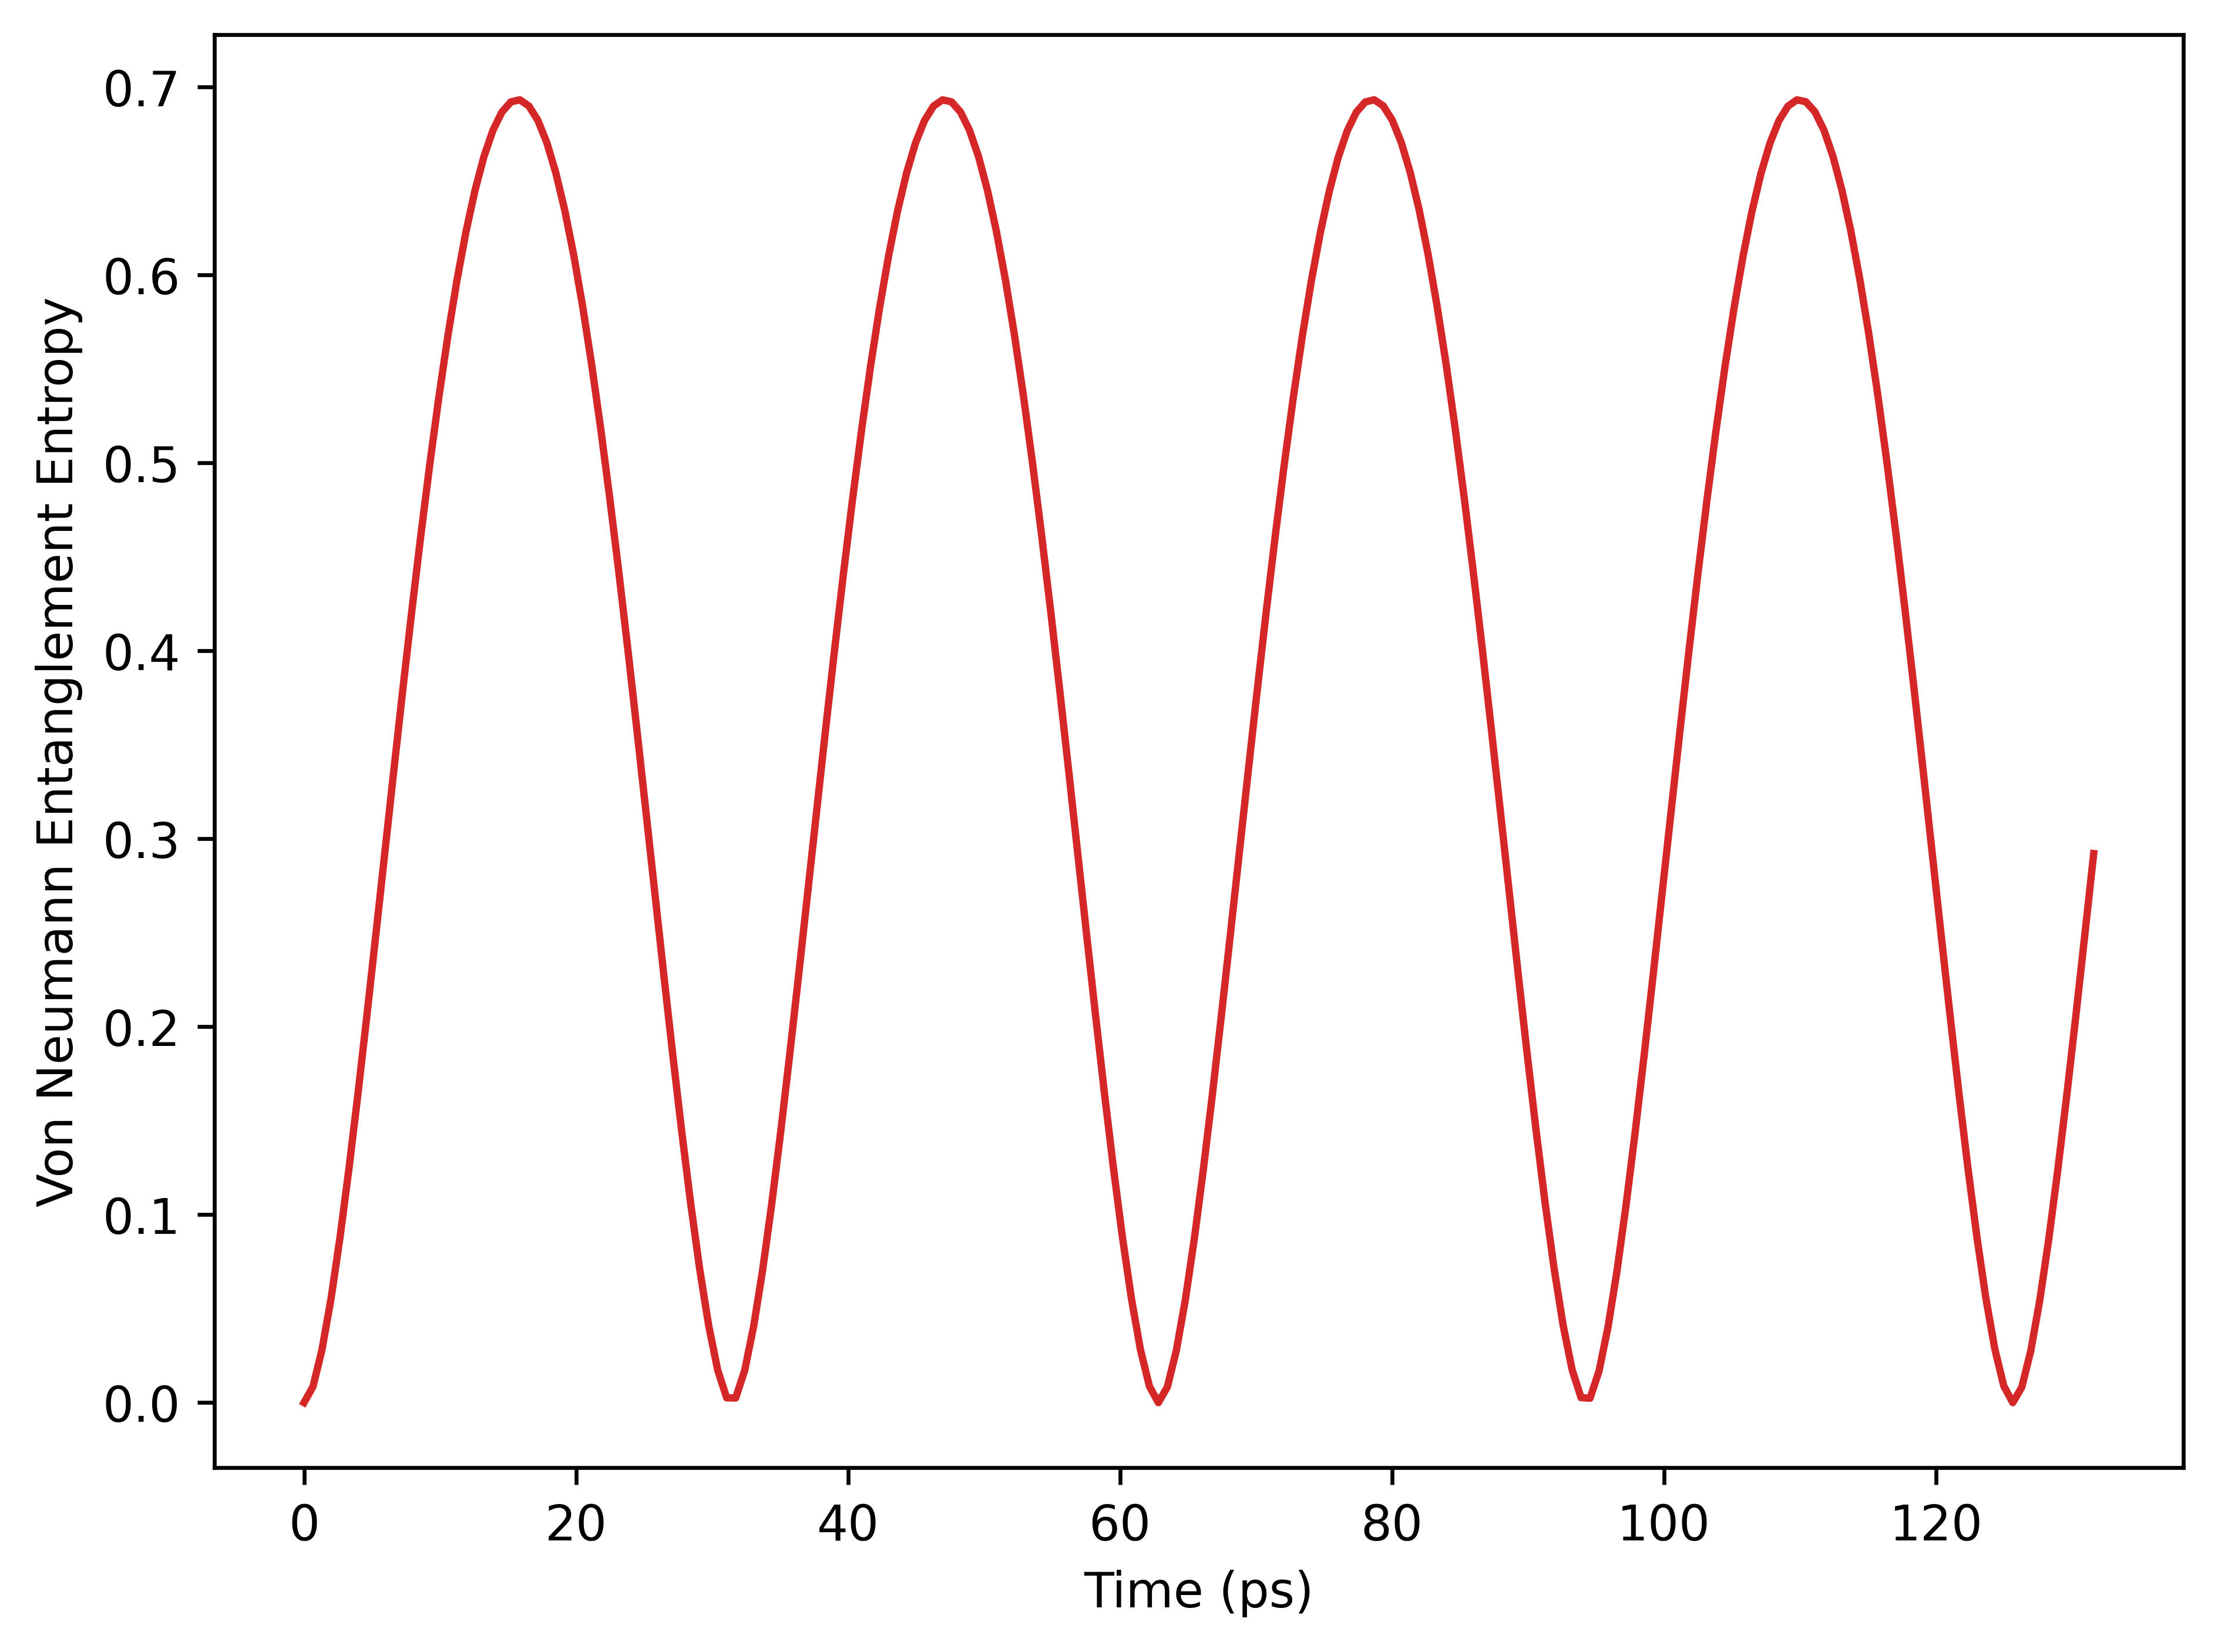
\includegraphics[width=\linewidth]{Research Project/Code/results/JCM/CQS_vne.png}
        \caption{}
        \label{fig:JCM_cqs_vne_e0}
    \end{subfigure}
    \begin{subfigure}{0.45\textwidth}
        \centering
        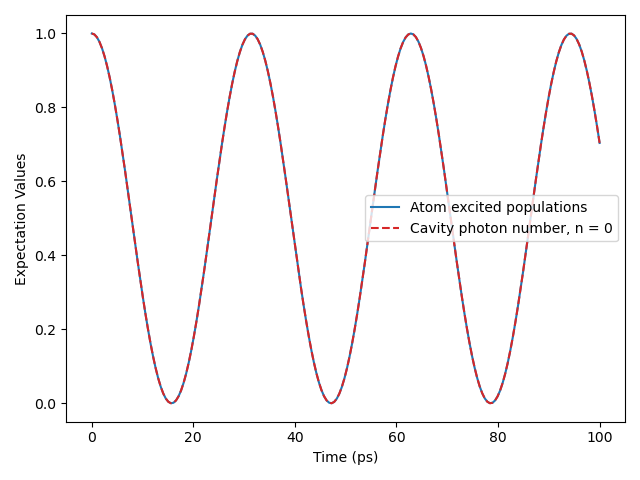
\includegraphics[width=\linewidth]{Research Project/Code/results/JCM/CQS_expt.png}
        \caption{}
        \label{fig:JCM_cqs_xpt_e0}
    \end{subfigure}

        \vspace{0.5cm}
    
    \begin{subfigure}{0.45\textwidth}
        \centering
        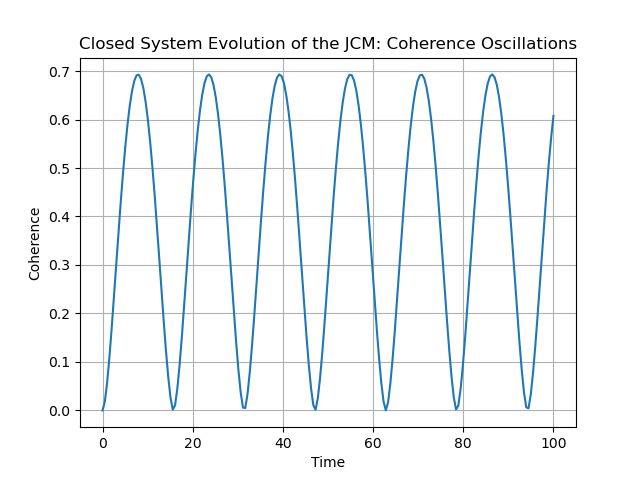
\includegraphics[width=\linewidth]{Research Project/Code/results/JCM/CQS_coh.png}
        \caption{}
        \label{fig:JCM_cqs_coh_e0}
    \end{subfigure}
    \hfill
    \caption{All figures above are simulations of the JCM under closed unitary evolution, starting in an initial state of $|\psi (\text{t=0})\rangle = |e, 0\rangle$. (a) Von Neumann entropy of the JCM. (b) Plot of the populations of the excited atomic state $|e\rangle$, and the cavity state, $|n=1\rangle$. (c) Relative entropy of coherence of the JCM.}
\end{figure}

In figure \ref{fig:JCM_cqs_vne_e0}, we can clearly see the oscillatory pattern of entanglement that we find from our analytical calculations. These oscillations are one of the key features of the JCM: Rabi oscillations. As mentioned in section \ref{sec:theory_subsub_JCM}, the oscillations come from the interaction part of the Hamiltonian:

\begin{equation*}
     \hat{H}_{\scriptscriptstyle \text{I}} = \hbar g(\hat{\sigma}_{+}\hat{a} +\hat{\sigma}_{-}\hat{a}^\dagger),
\end{equation*}

which drives coherent exchange of excitations between the atom and field. The term $\hat{\sigma}_{+}\hat{a}$ describes photon absorption resulting in atomic excitation, whilst $\hat{\sigma}_{-}\hat{a}^\dagger$ corresponds to photon emission with atomic de-excitation. Since $\hat{H}_{\scriptscriptstyle\text{I}}$ commutes with the total excitation number operator, $\hat{N} = \hat{a}^\dagger \hat{a} + \frac{1}{2}(1 + \hat{\sigma}_z)$, evolution is confined to subspaces of fixed $\hat{N}$. So, for the initial state $|e,0\rangle$ where $\hat{N} = 1$, the dynamics occur entirely within the space \small{\{$|g,1\rangle,|e,0\rangle$\}}, producing Rabi oscillations at frequency g. This periodic transfer causes modulation in the entanglement, between  0 (pure states) and $\ln2$ (maximal entanglement for a TLS).\\
\\
We can directly see these Rabi oscillations in figure \ref{fig:JCM_cqs_xpt_e0}. At time $t = 0$, the populations of the excited state of the atom $|e\rangle$ and the cavity at  $|n=1\rangle$ start off in our initial state as expected. From there, since the dynamics are restricted to \small{{$|g,1\rangle,|e,0\rangle$}}, the system exhibits periodic transfer of excitation between the atom and the field and completely transfers the population at each half-period at the Rabi frequency $g$.\\
\\
Now that we have explored the von Neumann entropy analytically and computationally, we complete our analytical goals by exploring the relative entropy of coherence. This measure of coherence, which we recall from equation \eqref{rel_ent_coh} is written as:


\begin{equation*}
C_r(\rho) = C_d(\rho) = S(\rho_{diag}) - S(\rho),
\end{equation*}

where $\rho_{diag}$ is obtained by removing all non-diagonal entries of the matrix $\rho$. We firstly look at $C_r(\rho_{\scriptscriptstyle \text{TLS}}(t)) \text{ and }  C_r(\rho_{\scriptscriptstyle \text{QHO}}(t))$, the relative entropy of coherence for both subsystems. By inspection of the density matrices in equation \eqref{eqn:subsys_JCM_closed}, we see that both subsystem matrices are diagonal. Thus, $S(\rho_{diag}) = S(\rho)$, and so their coherences are $0$. For the total system, however, the result is non-trivial. We start by calculating the second term, $S(\rho(t))$, by diagonalising our density matrix in \eqref{eqn:JCM_dm(t)_closed}.
\begin{equation*}
    \det(\rho(t) - \lambda I) = 0,
\end{equation*}
and so 
\begin{equation*}
    \left(|\alpha(t)|^2\ - \lambda\right) \left(|\beta(t)|^2\ - \lambda \right) - |\alpha(t)|^2|\beta(t)|^2 =0
\end{equation*}

Solving for the eigenvalues $\lambda$, we get $\lambda_1 = 0$ and $\lambda_2 = |\alpha(t)|^2 + |\beta(t)|^2$. We know that, for a valid pure density matrix, $\text{Tr}(\rho(t)) = 1$, so $\lambda_2 = 1$. Using equation \eqref{vne_eqn},

\begin{equation*}
    S(\rho(t)) = - 0 \ln0 - 1\ln1 = 0, 
\end{equation*}

and therefore $C_r(\rho(t)) = S(\rho_{diag}(t))$. Removing the off--diagonals from $\rho(t)$ gives

\begin{equation*}
    \rho_{diag}(t) = |\alpha(t)|^2|g,1\rangle\langle g,1| + |\beta(t)|^2|e,0\rangle\langle e,0|,
\end{equation*}

so that

\begin{equation*}
    S(\rho_{diag}(t)) = - |\alpha(t)|^2\ln(|\alpha(t)|^2) - |\beta(t)|^2\ln(|\beta(t)|^2) = C_r(\rho(t)).
\end{equation*}
\\
Both $|\alpha(t)|^2$ and $|\beta(t)|^2$ are the same as equation \eqref{eqn:JCM_complex_coeffs}, and so we find that for the total system, $C_r(\rho(t))$
oscillates between $0$ and $\ln2$. We again verify these coherence results in the closed evolution simulations of the JCM.

The system starts off in a pure state in figure \ref{fig:JCM_cqs_coh_e0}, and there are initially no off-diagonal elements and coherence is thus 0 for the total system. However, as the population begins to transfer between the states $|e,0\rangle,|g,1\rangle$, superpositions of these basis states develop. This produces non-zero off-diagonal terms in the computational basis, corresponding to coherence. The coherence reaches its maximum value of $\ln2$ when the system is in an equal superposition of the basis states, consistent with our theoretical analysis. \\
\\
We have completed our theoretical analysis of the JCM under closed evolution, successfully finding and verifying results for the von Neumann entropy and relative entropy of coherence, as well as plotting the populations for comparison. We now carry out the computational analysis of the second initial state from equation \eqref{init_JCM_e0g0}, which reads:

\begin{equation*}
    |\psi (\text{t=0})\rangle = \frac{1}{\sqrt{2}}(|e, 0\rangle + |g,0\rangle).
\end{equation*}

This initial state contains the $|g,0\rangle$ component, which is effectively stationary. In the JCM, the only allowed couplings are betweeen $|e,n\rangle,$ and $|g,n+1\rangle$ due to excitation number conservation. There is no lower photon state for $|g,0\rangle$ couple to,  so it remains unchanged during the evolution. The $|e,0\rangle$ component, however, will evolve in the same manner as the previously considered initial state. 

We expect that there will be entanglement in the system, since the component $|e,0\rangle$ will, during its transition into the $|g,1\rangle$, be in some linear combination of $|e,0\rangle$ and $|g,1\rangle$. 

We also anticipate that both the subsystems and the total system will exhibit coherence, as the initial state is a superposition. Consequently, the subsystems should contain off--diagonal terms.\\
\begin{figure}[h]
    \centering
    \begin{subfigure}{0.45\textwidth}
        \centering
        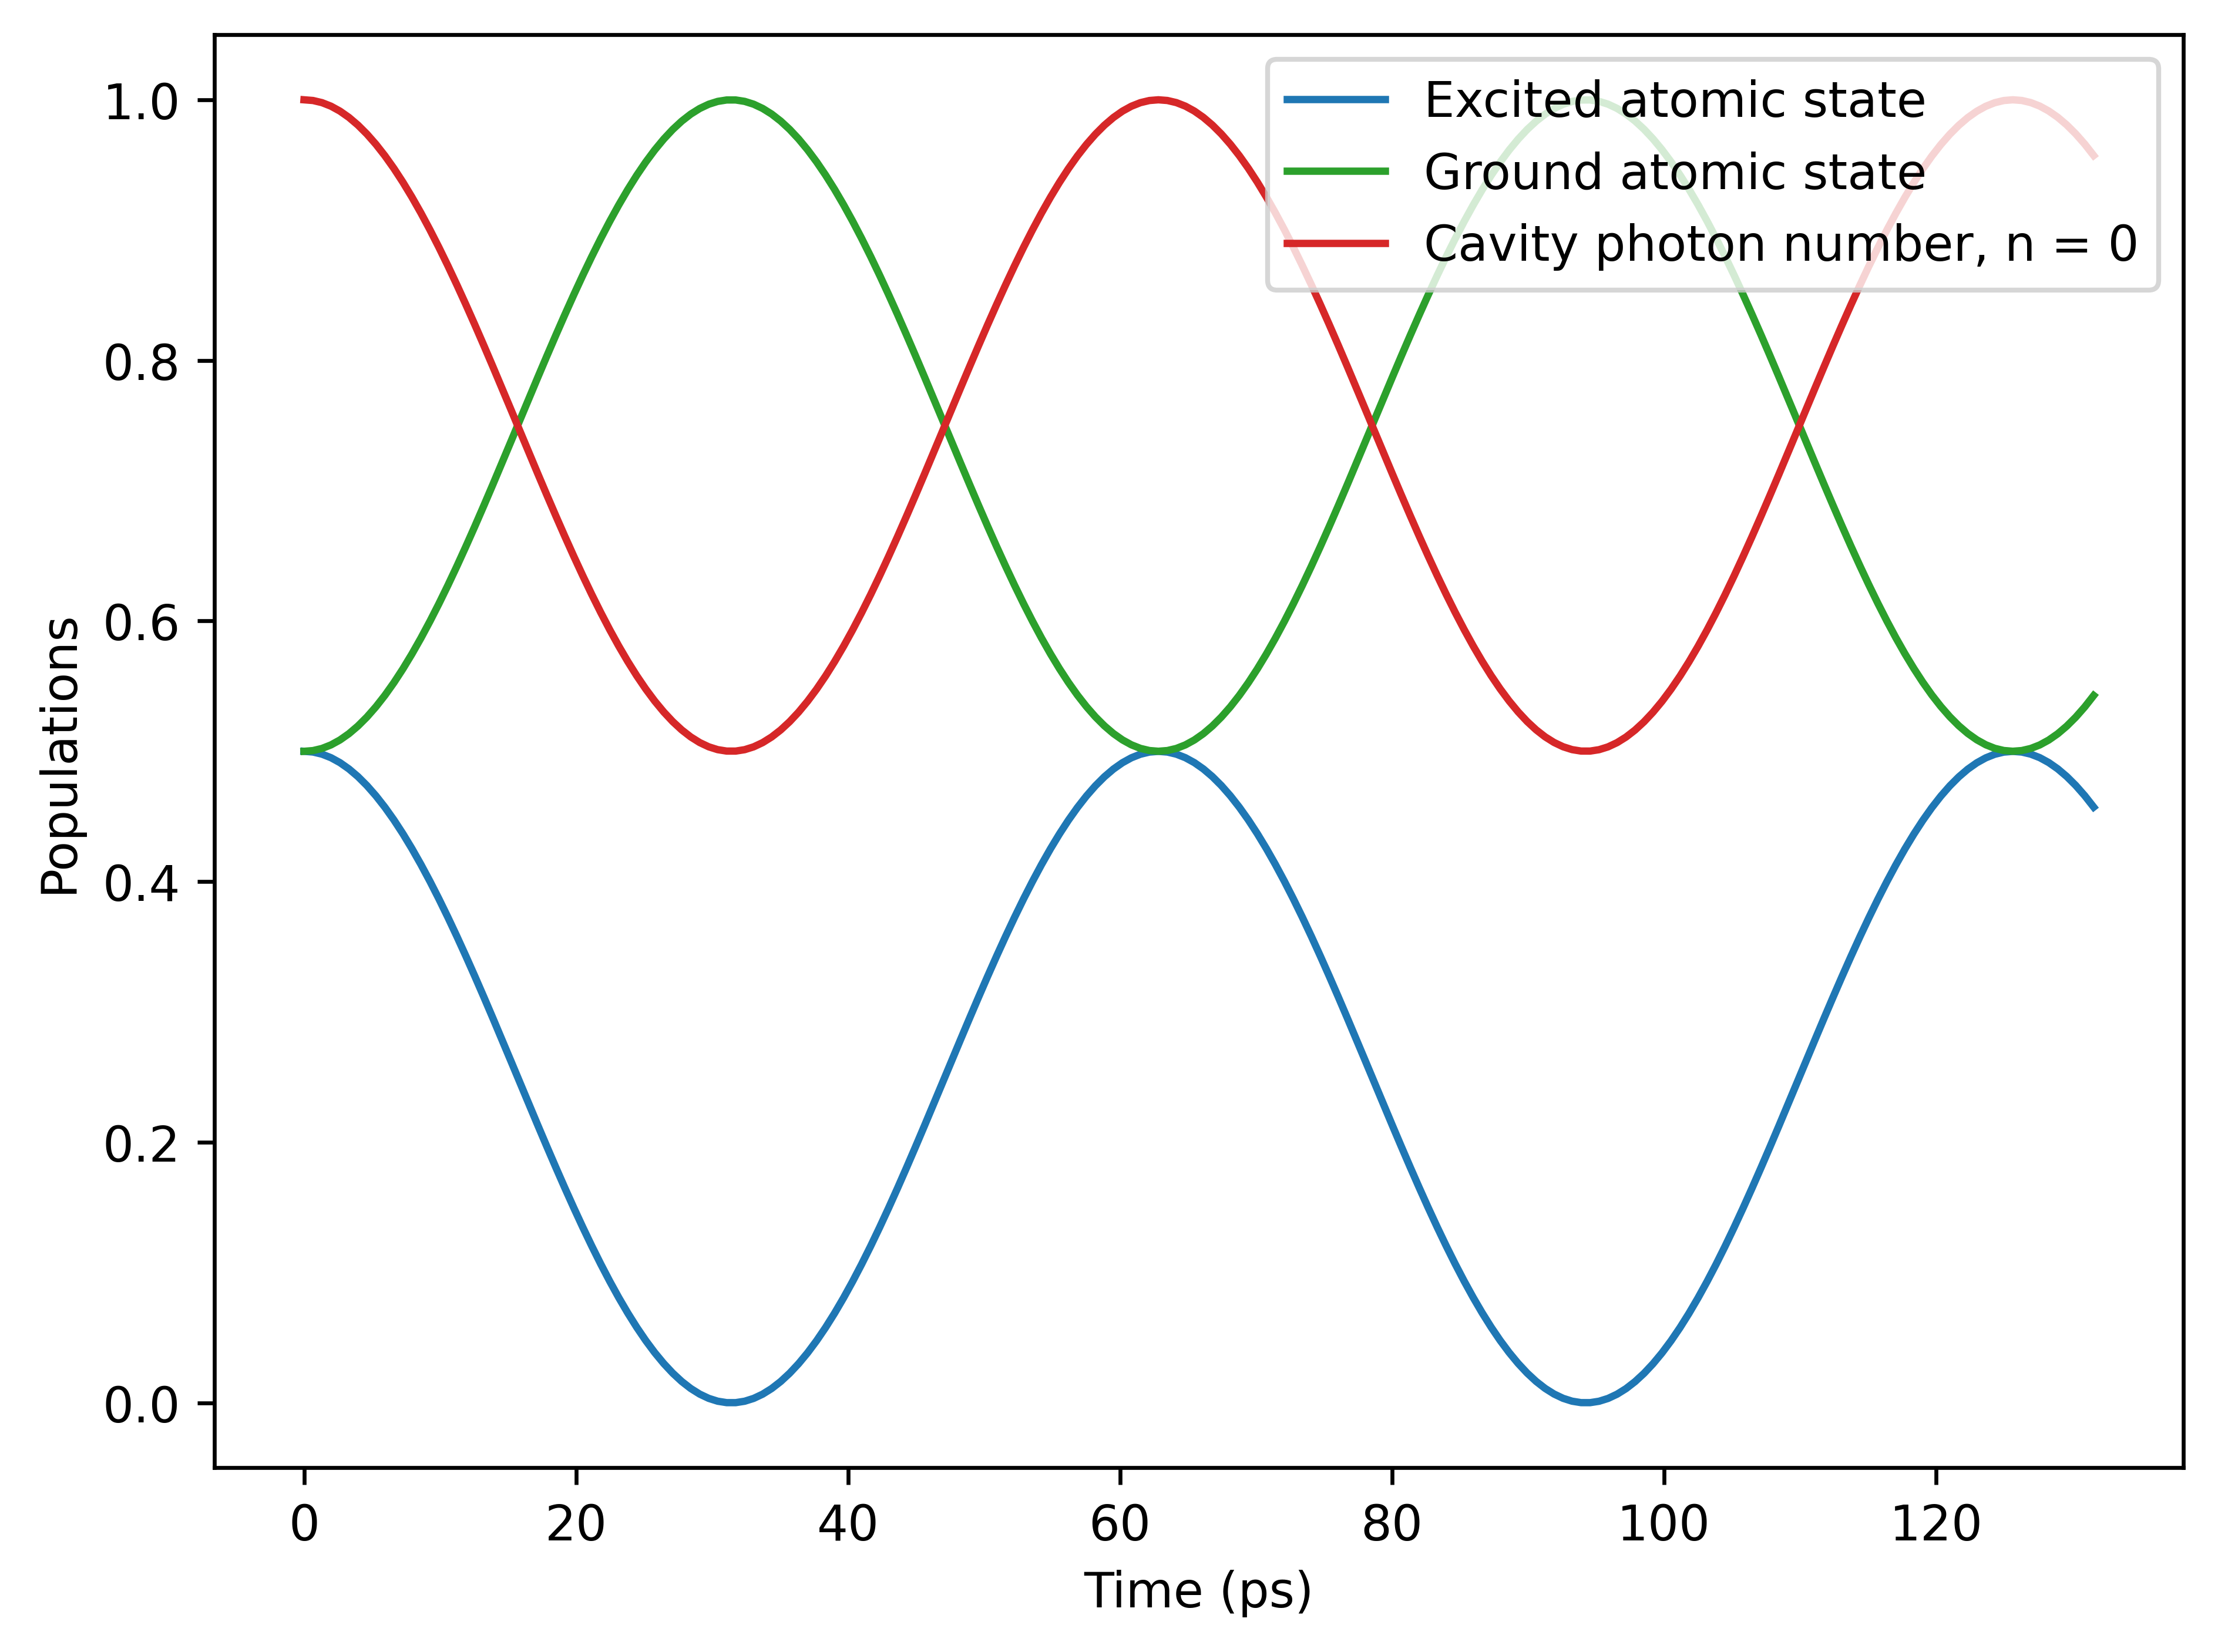
\includegraphics[width=\linewidth]{Research Project/Code/results/JCM/CQS_expt_eg.png}
        \caption{}
        \label{fig:jcm_cqs_expt_eg}
    \end{subfigure}
    \hfill
    \begin{subfigure}{0.45\textwidth}
        \centering
        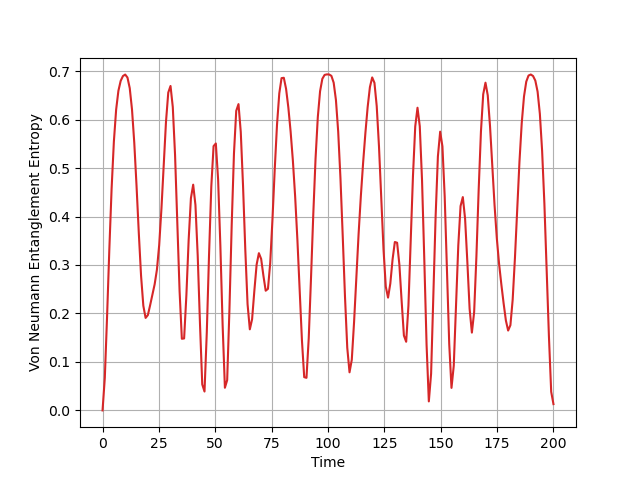
\includegraphics[width=\linewidth]{Research Project/Code/results/JCM/CQS_vne_eg.png}
        \caption{}
        \label{fig:jcm_cqs_vne_eg}
    \end{subfigure}
    
    \vspace{0.5cm}
    
    \begin{subfigure}{0.45\textwidth}
        \centering
        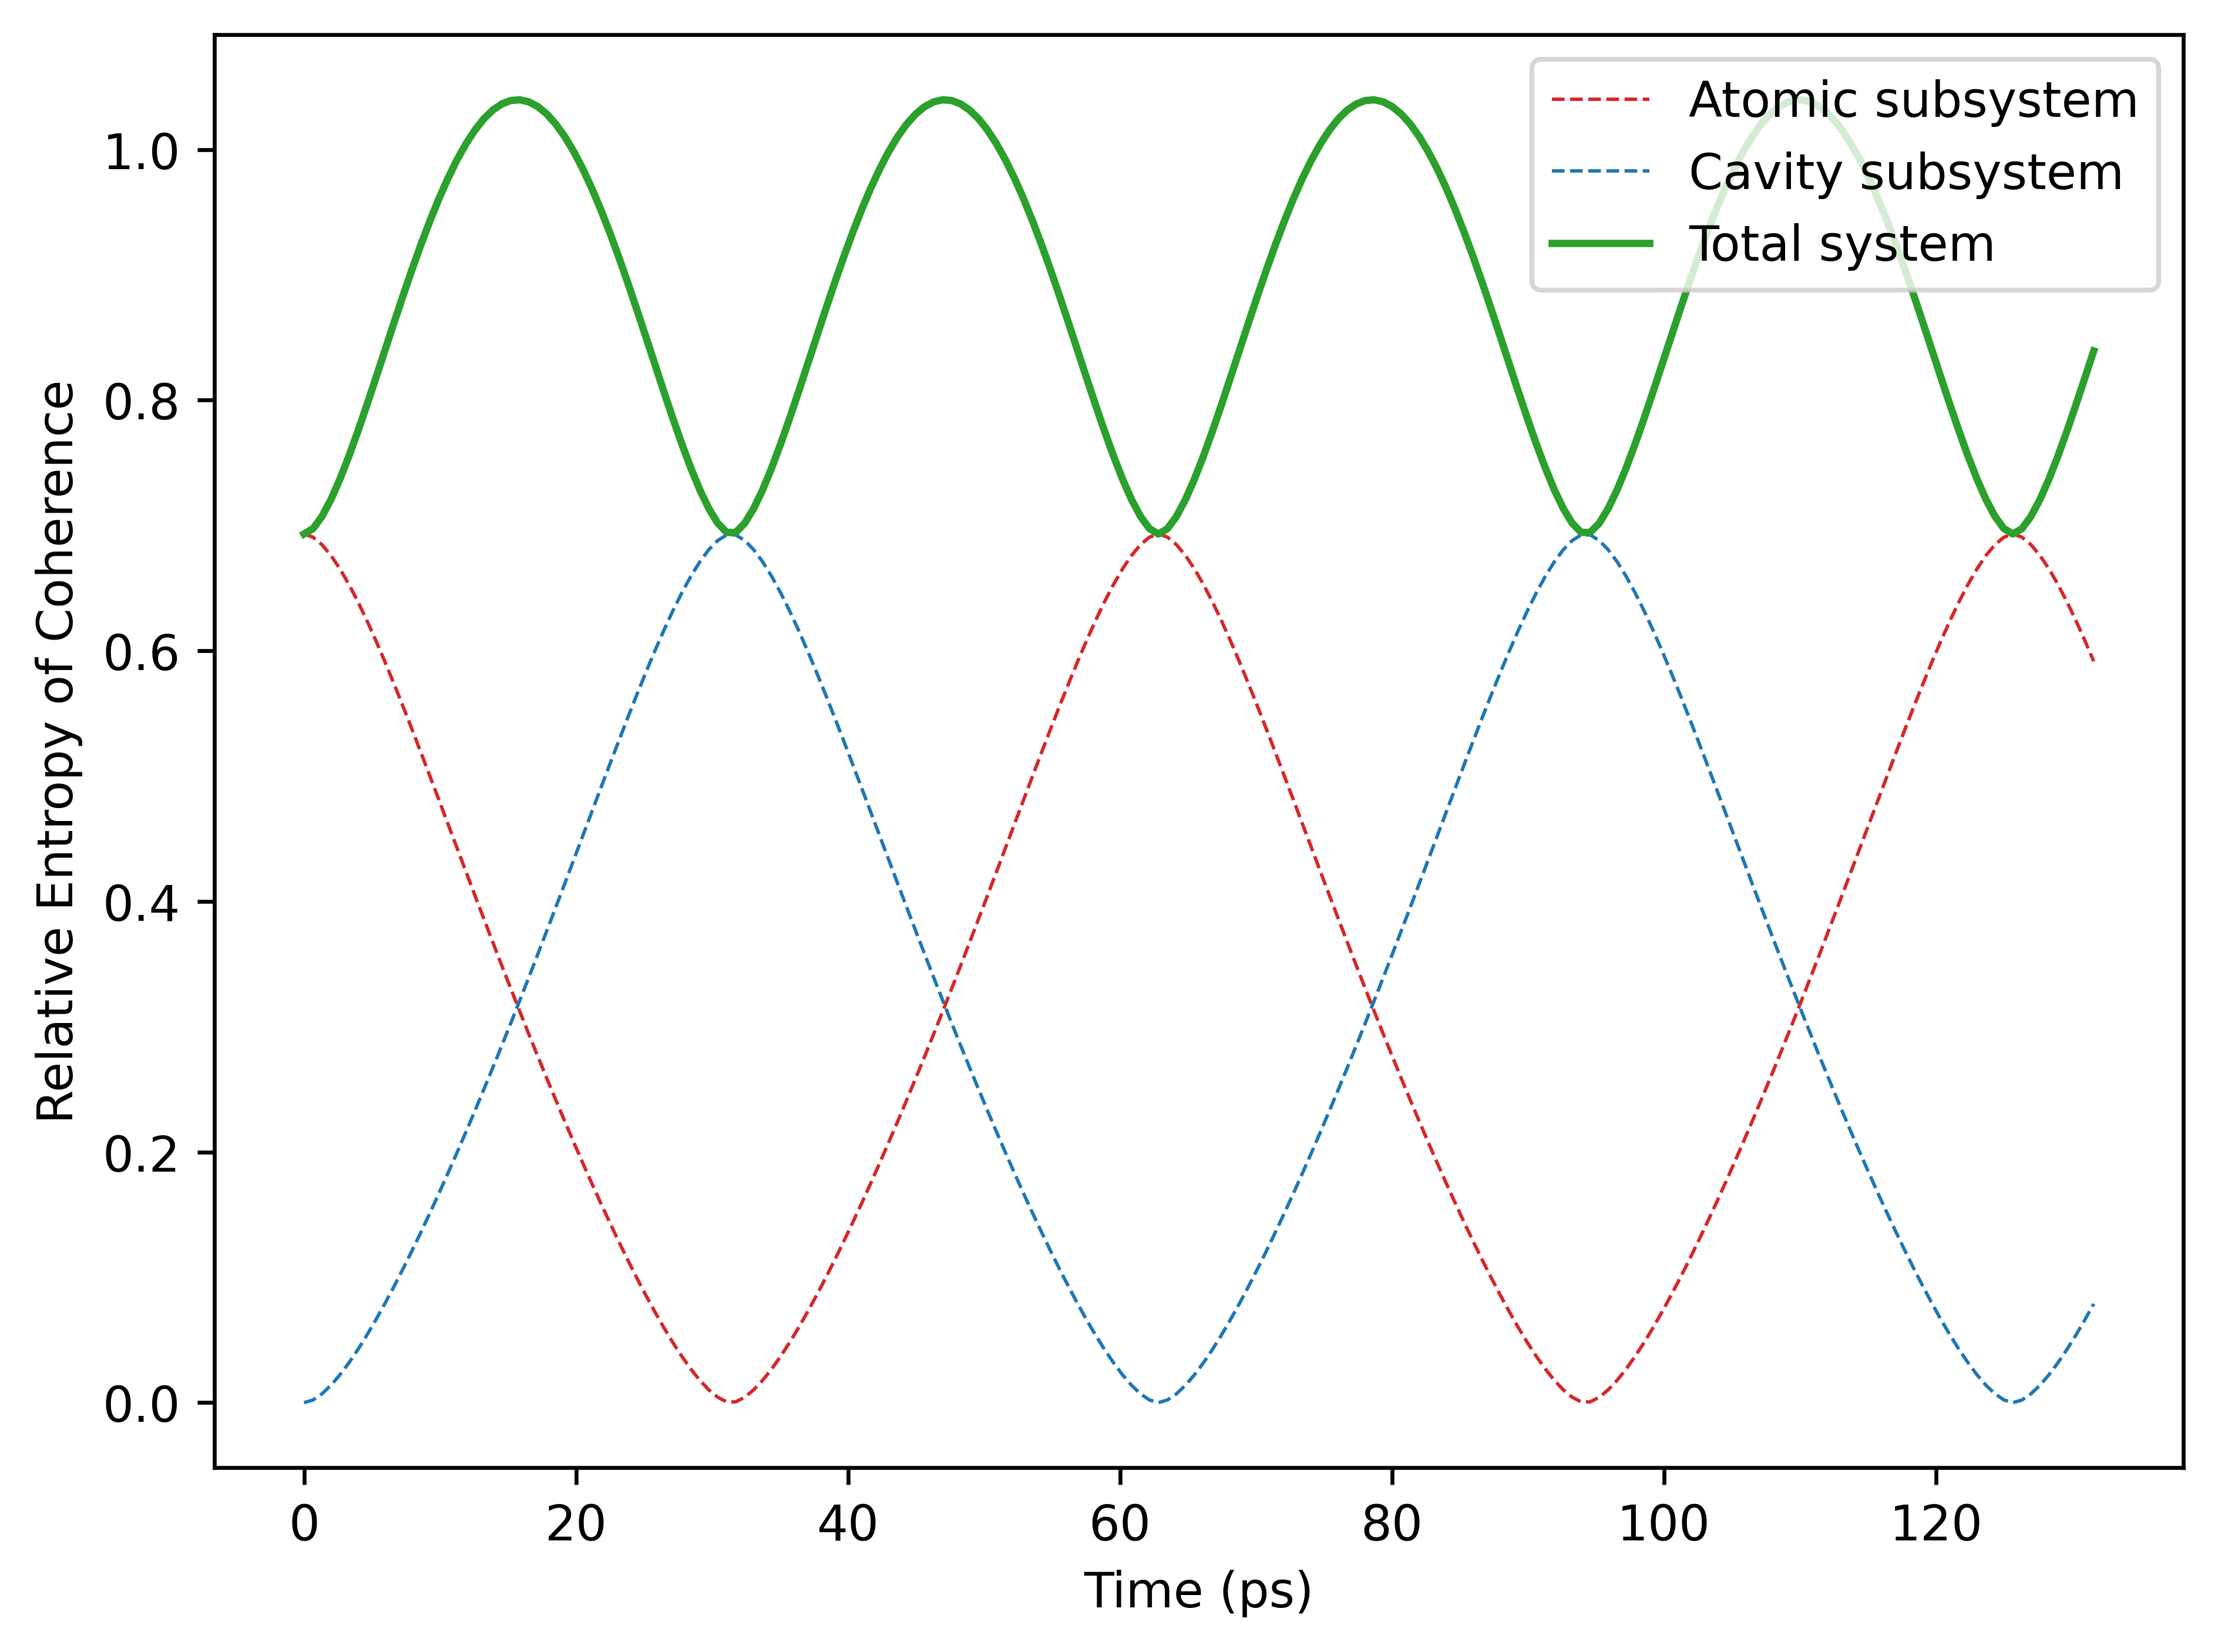
\includegraphics[width=\linewidth]{Research Project/Code/results/JCM/CQS_coh_eg.png}
        \caption{}
        \label{fig:jcm_cqs_coh_eg}
    \end{subfigure}
    \hfill

    \caption{All figures above are simulations of the JCM under closed unitary evolution, starting in an initial state of $|\psi (\text{t=0})\rangle = \frac{1}{\sqrt{2}}(|e, 0\rangle + |g,0\rangle)$. (a) Plot of the populations of the excited atomic state $|e\rangle$, the ground atomic state $|g\rangle$ and the cavity state, $|n=0\rangle$. (b) Von Neumann entropy of the JCM. (c) Plot of the relative entropy of coherence for the two subsystems and the total system.}
    \label{fig:JCM_cqs_e0g0}
\end{figure}

We start by analysing figure \ref{fig:jcm_cqs_expt_eg}, which shows the populations of the ground and excited state of the atom, and the cavity state population of the $|n=1\rangle$ fock state. As expected, the $|g,0\rangle$ component of the initial state is stationary, and so there will always be a non-zero contribution to the populations of $|g\rangle$ and $|n=0\rangle$. At $t\approx 30\text{ps}$, we see that half the population of the cavity is transferred to $|n=1\rangle$, and for the atom, to $|g\rangle$. This illustrates the expected Rabi oscillation dynamics, where the excitation initially in the $|e,0\rangle$ state is transferred coherently to the $|g,1\rangle$ state. \\
\\
As expected, there is entanglement in the system, characterised by the von Neumann entropy (figure \ref{fig:jcm_cqs_vne_eg}). It exhbits the same oscillations as the previous initial state's entanglement characteristics due to the Rabi oscillations in the populations. Furthermore, entanglement is maximal during the transition of the $|e,0\rangle$ component to $|g,1\rangle$ which matches our predictions. However, the range of entanglement is much lower (between 0 and 0.25 as compared to 0 and 0.7 in figure \ref{fig:JCM_cqs_vne_e0}. This could be attributed to entanglement being diluted by the $|g,0\rangle$ component. The $|g,0\rangle$ component remains stationary, never mixes with the other components, and effectively behaves as an unentangled product state.
In terms of the von Neumann entropy, this stationary, classically--behaving fraction of the total state limits the entanglement achieved during evolution.\\
\\
Finally, we observe coherence in the full system, $C_r(\rho(t))$. Although this behaviour resembles that of our previous initial condition,  the presence of the stationary component leads to some key differences. The stationary component $|g,0\rangle$ adds an off--diagonal term to our full system, thus creating a baseline level of coherence throughout the evolution. This causes the minimum of $C_r(\rho(t))$ is approximately 0.5, whereas previously it was 0. Moreover, it raises the maximum value of $C_r(\rho(t))$. We also observe coherences in both subsystems. To see why there is coherence in the initial state for the atomic subsystem, but not the cavity subsystem, let us analyse the initial condition's subsystems.

\begin{equation*}
    |\psi(t=0)\rangle = \frac{1}{\sqrt{2}}\left(|e,0\rangle + |g,0\rangle\right),
\end{equation*}

so its density matrix is

\begin{equation*}
    |\rho(t=0)\rangle = \frac{1}{2}\left(|e,0\rangle\langle e,0| + |g,0\rangle\langle g,0| + |e,0\rangle\langle g,0| + |g,0\rangle\langle e,0| \right).
\end{equation*}

The atomic subsystem is found by taking the partial trace:

\begin{equation*}
    \rho_{\scriptscriptstyle \text{TLS}}(t = 0) = \frac{1}{2}\left(|e\rangle\langle e|+ |g\rangle\langle g|+|e\rangle\langle g|+|g\rangle\langle e|\right),
\end{equation*}

and so we expect there to be coherence in this subsystem initially. For the cavity subsystem, however, 

\begin{equation*}
    \rho_{\scriptscriptstyle \text{QHO}}(t = 0) = \left(|0\rangle\langle 0|\right),
\end{equation*}

which is a diagonal matrix and thus has no coherence at t=0. The coherence values for each subsystem oscillates between 0 and 0.7, which matches our expectations due to the population transfers caused by Rabi oscillations. 

%Whilst exactly how coherence and entanglement may be utilised experimentally in TLS--QHO systems is beyond the scope of this study, we have shown that coherence in TLS--QHO



\newpage
\subsubsection{Open Evolution}

We start with our first initial state in equation \eqref{init_JCM_e0}. Let us start by analysing the populations of the subsystems. 

\begin{figure}[H]
    \centering
    \begin{subfigure}{0.45\textwidth} 
        \centering
        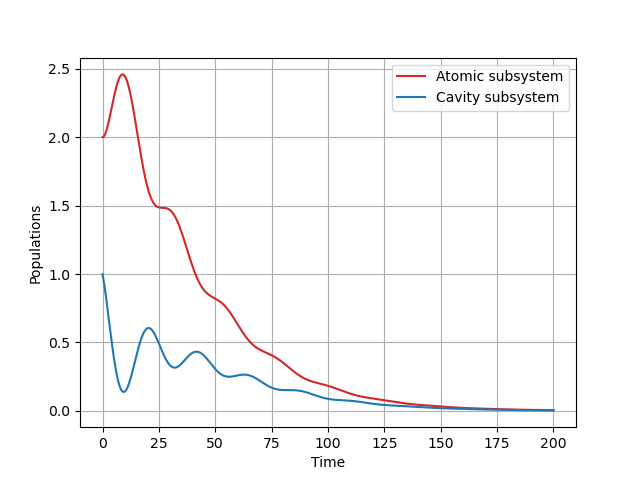
\includegraphics[width=\linewidth]{Research Project/Code/results/JCM/OQS_Pop_Spont.png}
        \caption{}
        \label{fig:JCM_OQS_Pop_Spont}
    \end{subfigure}
    \hfill
    \begin{subfigure}{0.45\textwidth}
        \centering
        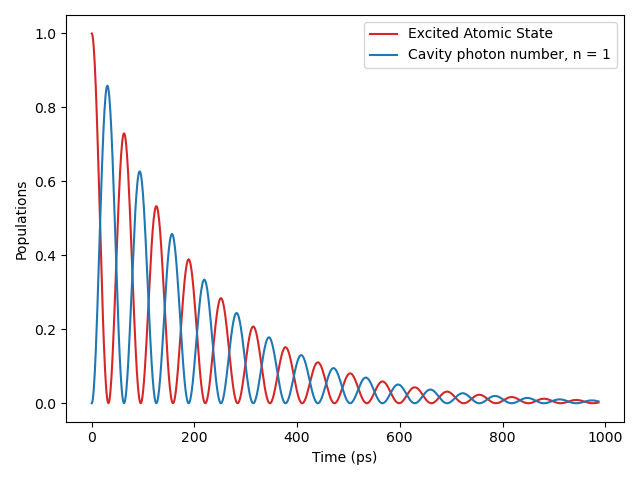
\includegraphics[width=\linewidth]{Research Project/Code/results/JCM/OQS_Pop_Therm.png}
        \caption{}
         \label{fig:JCM_OQS_Pop_Therm}
    \end{subfigure}
    
    \vspace{0.5cm}
    
    \begin{subfigure}{0.45\textwidth} 
        \centering
        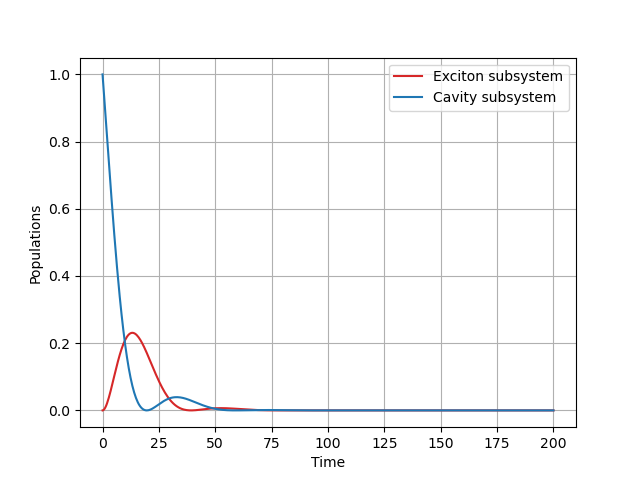
\includegraphics[width=\linewidth]{Research Project/Code/results/JCM/OQS_Pop_Both.png}
        \caption{}
         \label{fig:JCM_OQS_Pop_Both}
    \end{subfigure}
    \hfill
    \caption{}
    \label{fig:JCM_OQS_Pop}
\end{figure}

Under all types of decays (see section \ref{sec:method_sub_JCM}), we observe Rabi oscillations as expected. However, the populations of both subsystems decay, due to loss to the environment. This decay is to be expected, and is a hallmark of open quantum evolution. Interestingly, the Rabi oscillations' period remains constant over all time, which is a consequence of the Rabi frequency $g$ not being a function of time. However, figures \ref{fig:JCM_OQS_Pop_Spont}, \ref{fig:JCM_OQS_Pop_Therm} show that the decays of both subsystems under either spontaneous atomic emission and thermal dissipation are almost identical. We can attribute this similarity to the low temperature regime, such that thermal dissipation is only associated with photon loss (see equation \eqref{eqn:L_therm}). This means that the decay operator for the dissipator is effectively only photon loss. Since, as mentioned in section \ref{sec:method_sub_JCM}, we have set the decay rates of the thermal and spontaneous emission to be equal ($\gamma = \gamma_{\scriptscriptstyle \text{th}} =0.01$, the two decay types are effectively equal (just acting on different subsystems). Moreover, the Rabi oscillations lead to decay in the other subsystems due to excitation transfer, a key characteristic in the JCM. Finally, we note that the two decays individually both lead to the populations being 0 around $t = 1000 ps$, for both decays acting simultaneously, we have the populations being 0 around $t = 600 ps$ in figure \ref{fig:JCM_OQS_Pop_Both}. As the Lindblad operators remove excitations, they suppress both diagonal and off--diagonal elements of the density matrix on comparable timescales. In this basis, coherence cannot outlive population, and so both decay together. We further not

\begin{figure}[H]
    \centering
    \begin{subfigure}{0.45\textwidth}
        \centering
        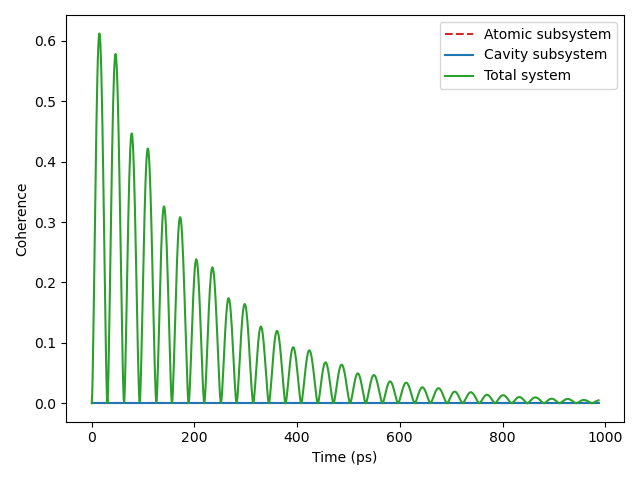
\includegraphics[width=\linewidth]{Research Project/Code/results/JCM/OQS_Coh_Spont.png}
        \caption{}
        \label{fig:JCM_OQS_Coh_Spont}
    \end{subfigure}
    \hfill
    \begin{subfigure}{0.45\textwidth}
        \centering
        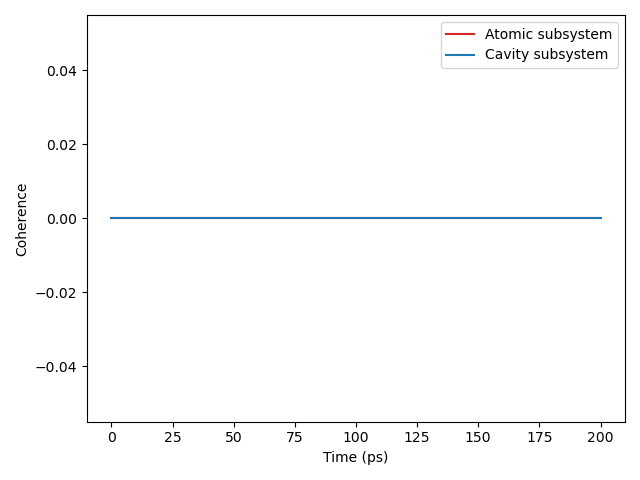
\includegraphics[width=\linewidth]{Research Project/Code/results/JCM/OQS_Coh_Therm.png}
        \caption{}
        \label{fig:JCM_OQS_Coh_Therm}
    \end{subfigure}
    
    \vspace{0.5cm}
    
    \begin{subfigure}{0.45\textwidth}
        \centering
        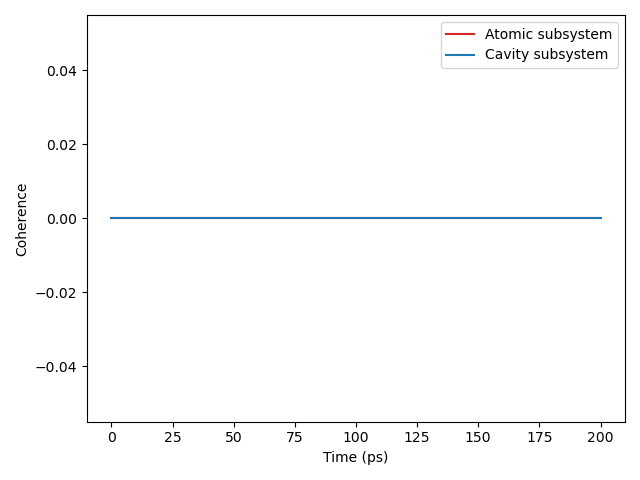
\includegraphics[width=\linewidth]{Research Project/Code/results/JCM/OQS_Coh_Both.png}
        \caption{}
        \label{fig:JCM_OQS_Coh_Both}
    \end{subfigure}
    \hfill
    \caption{}
    \label{fig:JCM_OQS_Coh}
\end{figure}

When talking about open quantum systems, a feature of such evolution that is key is decoherence, which, as mentioned in section \ref{sec:theory_sub_OQS}, is the decay of the off--diagonals of a system, leading to a loss of 'quantumness'. We can observe this directly by looking at the decay of coherence. For the total system, in the computational basis $\{|e,0\rangle, |g,1\rangle\}$, there is coherence in the closed system evolution, so we expect coherence as well for the open system evolution. We indeed observe this. For all types of decay, the total system's coherence decays on the same timescales as the populations, around $t \approx 1000ps$ for spontaneous emission and thermal dissipation (figures \ref{fig:JCM_OQS_Coh_Spont}, \ref{fig:JCM_OQS_Coh_Therm}), and $ t \approx 600ps$ for both decay channels open simultaneously (figure \ref{fig:JCM_OQS_Coh_Both}). As the Lindblad operators act to decay excitations, they suppress both diagonal and off–diagonal elements of the density matrix on comparable timescales. In this basis, coherence cannot outlive population, and so the system decoheres.\\
\\
\begin{figure}[H] 
    \centering
    \begin{subfigure}{0.45\textwidth}
        \centering
        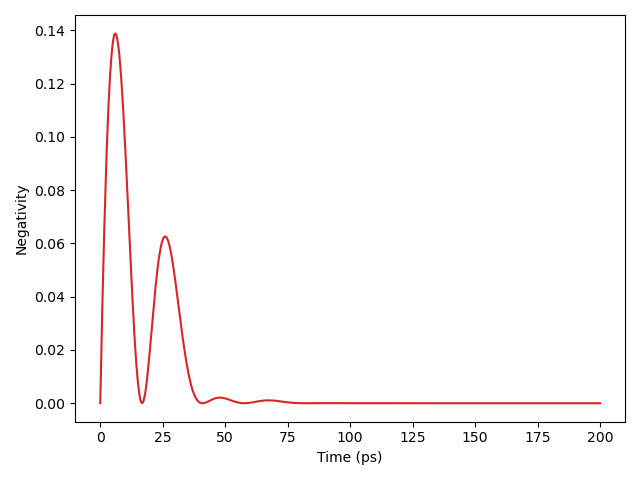
\includegraphics[width=\linewidth]{Research Project/Code/results/JCM/OQS_Neg_Spont.png}
        \caption{}
        \label{fig:JCM_OQS_Neg_Spont}
    \end{subfigure}
    \hfill
    \begin{subfigure}{0.45\textwidth}
        \centering
        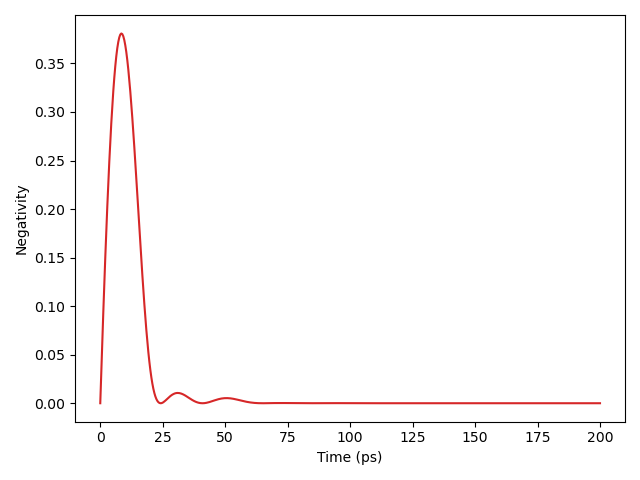
\includegraphics[width=\linewidth]{Research Project/Code/results/JCM/OQS_Neg_Therm.png}
        \caption{}
        \label{fig:JCM_OQS_Neg_Therm}
    \end{subfigure}
    
    \vspace{0.5cm}
    
    \begin{subfigure}{0.45\textwidth}
        \centering
        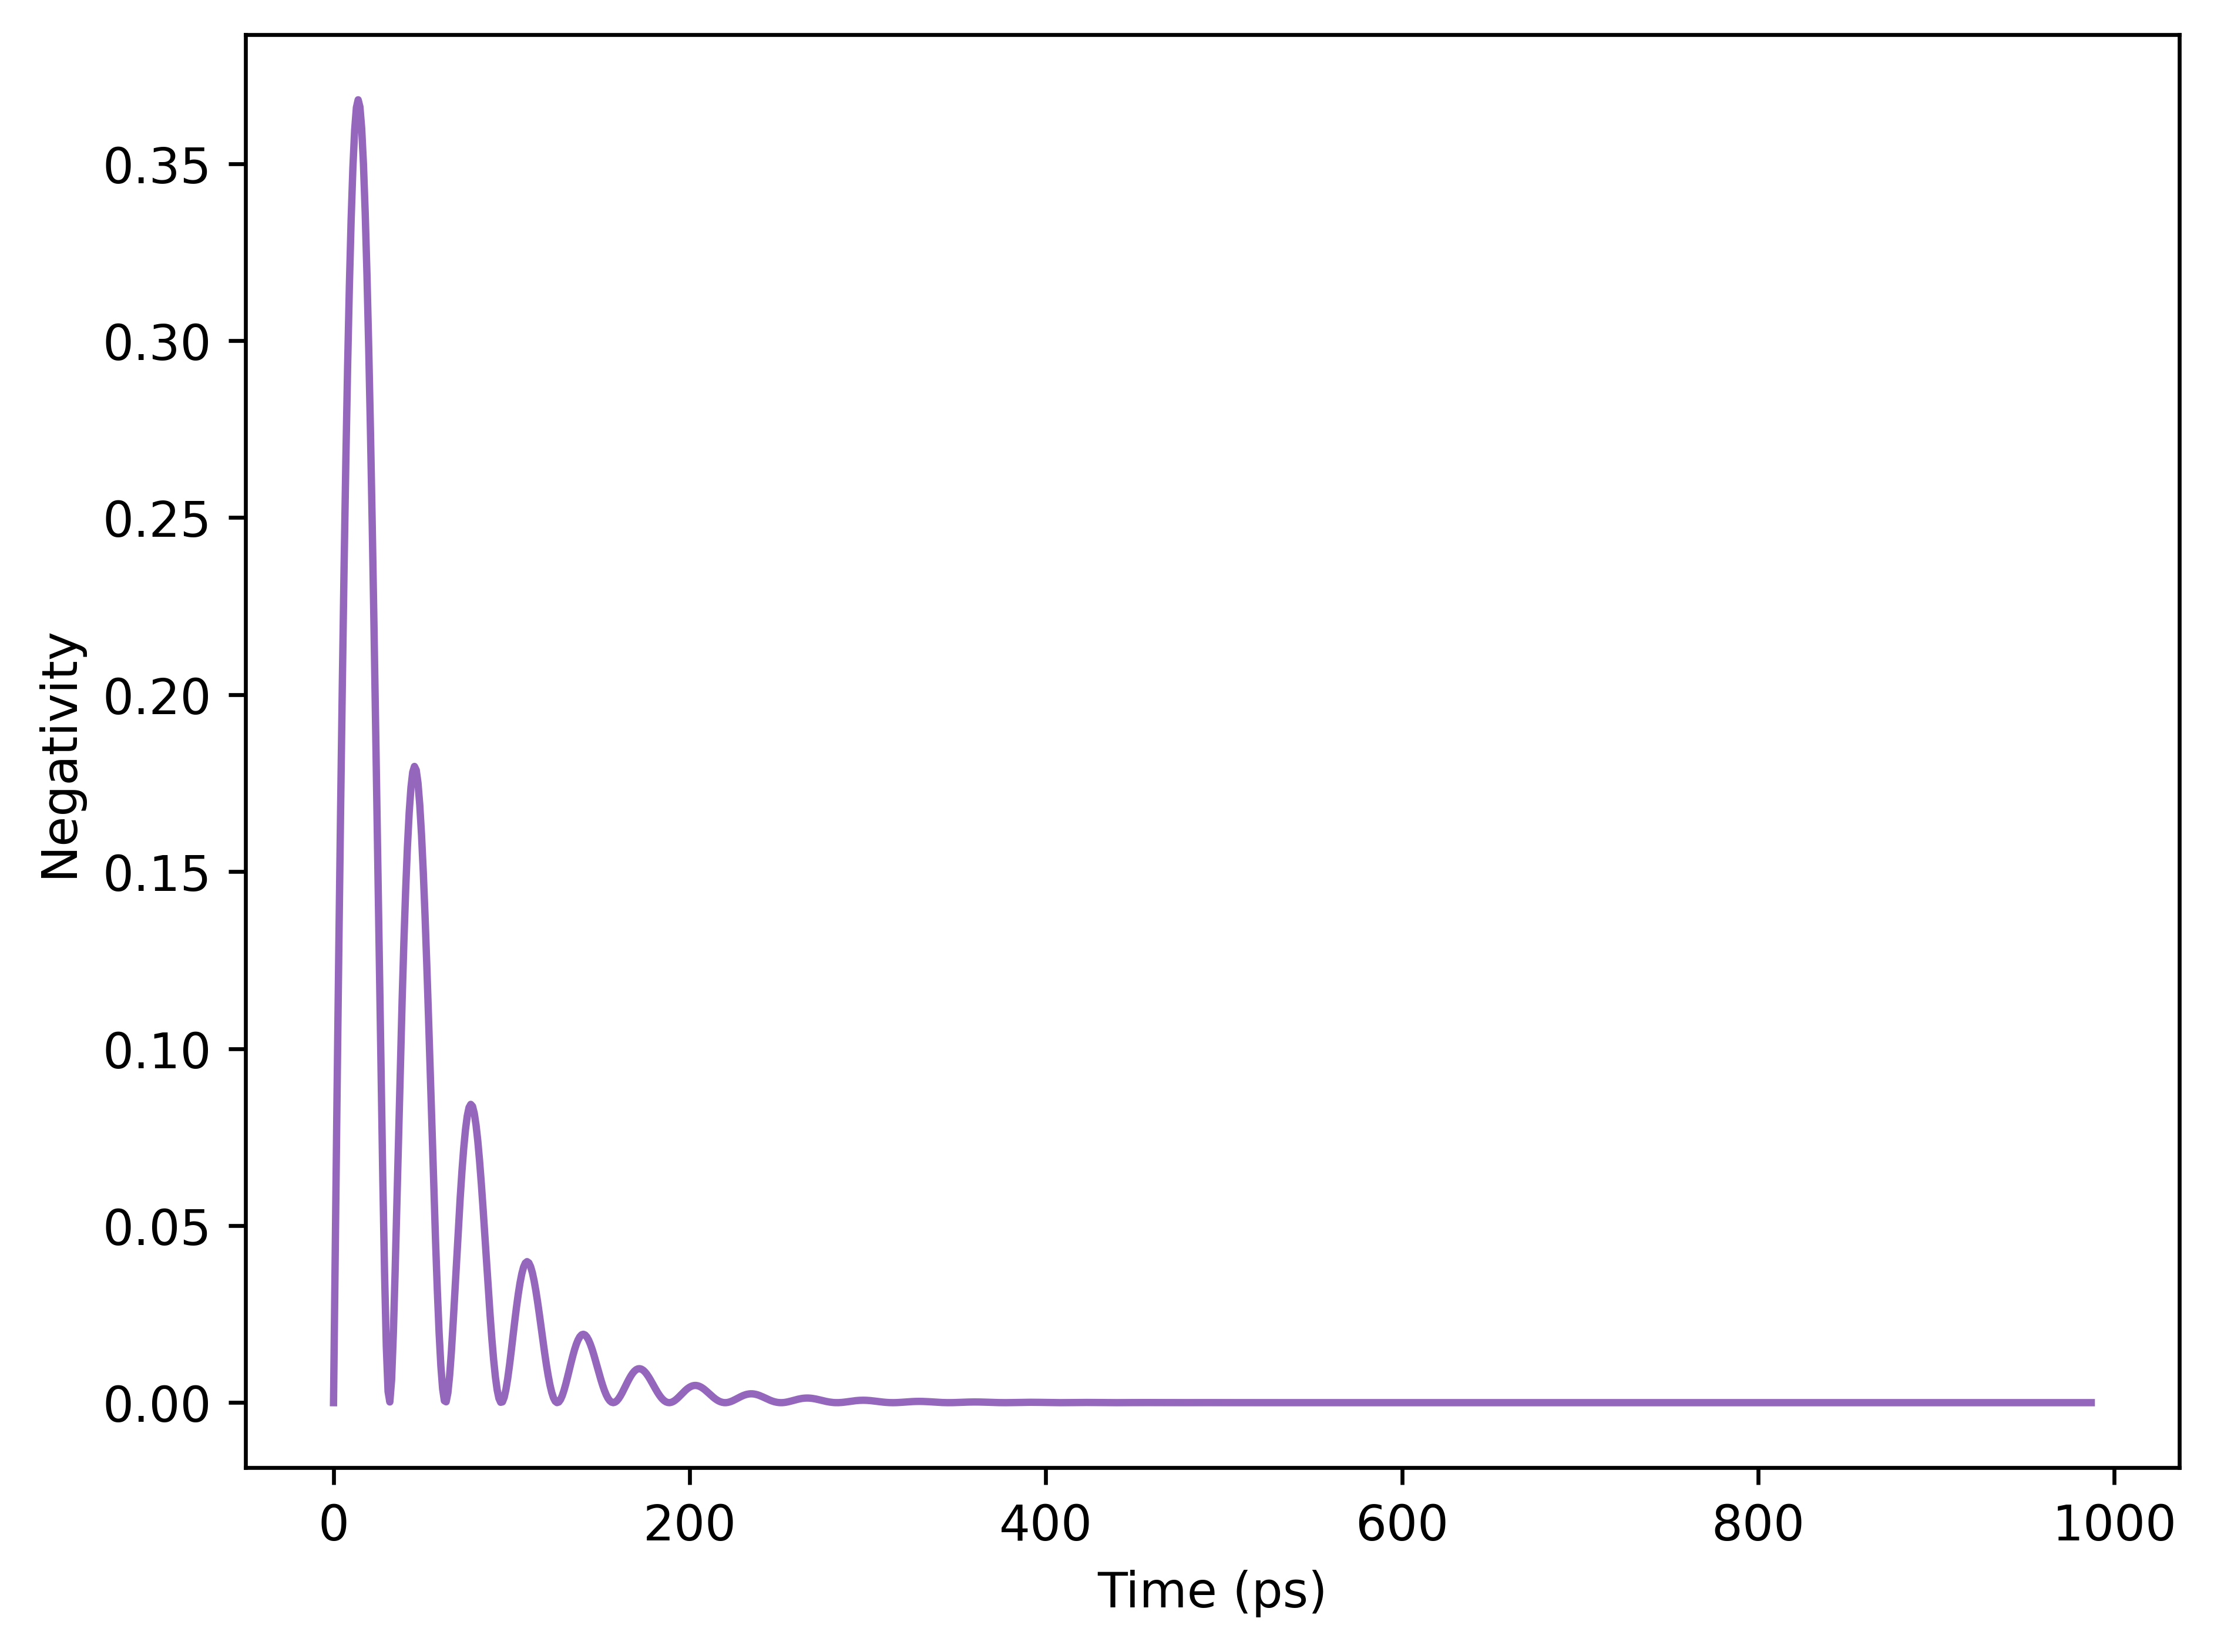
\includegraphics[width=\linewidth]{Research Project/Code/results/JCM/OQS_Neg_Both.png}
        \caption{}
        \label{fig:JCM_OQS_Neg_Both}
    \end{subfigure}
    \hfill
    \caption{}
    \label{fig:JCM_OQS_Neg}
\end{figure}

To conclude our simulations of the JCM, we look at the Negativity of the system. Figure \ref{fig:JCM_OQS_Neg} shows that negativity decays on a timescale approximately twice as fast as the population for all types of decay. This can be understood by noting that entanglement requires simultaneous occupation of both states $|e,0\rangle$ and $|g,1\rangle$. We may understand this by looking at one decay channel; let us look at the spontaneous emission. For entanglement to persist, both states must be populated at the same time. However, spontaneous emission acts directly on the excited atomic state, $|e,0\rangle$  and due to Rabi oscillations exchanging excitations, the $|g,1\rangle$ state is also gradually suppressed. Thus, the superposition of both is effectively decaying twice as fast and so we see a doubled decay rate for entanglement. The same process occurs with the thermal dissipation decay channel, except that now, the single photon state $|g,1\rangle$ is directly damped by photon loss, and through Rabi oscillations the $|e,0\rangle$ component is also gradually depleted. Finally, due to both decay channels being open for figure \ref{fig:JCM_OQS_Neg_Both}, we observe a decay time of half of that for either of the subsystems being open. \\
\\
As with the closed simulation, we also consider the second initial state in equation \eqref{init_JCM_e0g0}.


\begin{figure}[H]
    \centering
    \begin{subfigure}{0.45\textwidth}
        \centering
        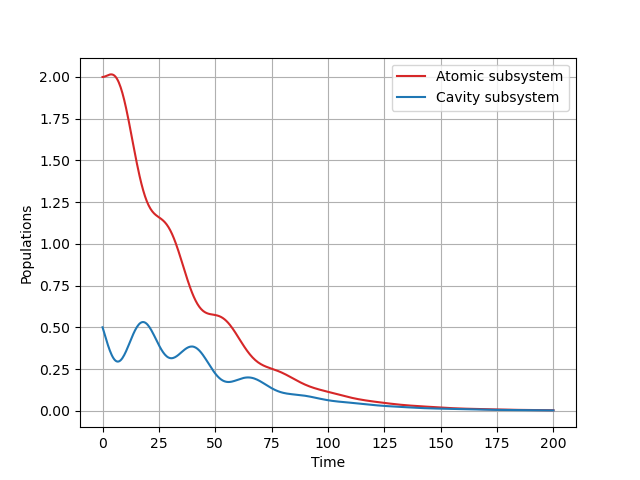
\includegraphics[width=\linewidth]{Research Project/Code/results/JCM/OQS_Pop_Spont_eg.png}
        \caption{}
        \label{fig:JCM_OQS_Pop_Spont_eg}
    \end{subfigure}
    \hfill
    \begin{subfigure}{0.45\textwidth}
        \centering
        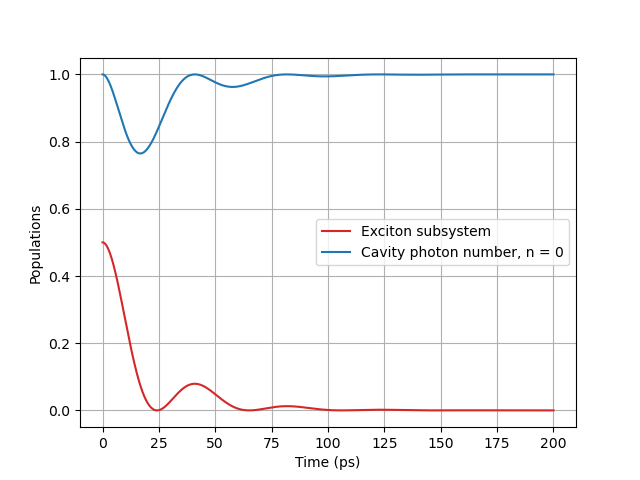
\includegraphics[width=\linewidth]{Research Project/Code/results/JCM/OQS_Pop_Therm_eg.png}
        \caption{}
        \label{fig:JCM_OQS_Pop_Therm_eg}
    \end{subfigure}
    
    \vspace{0.5cm}
    
    \begin{subfigure}{0.45\textwidth}
        \centering
        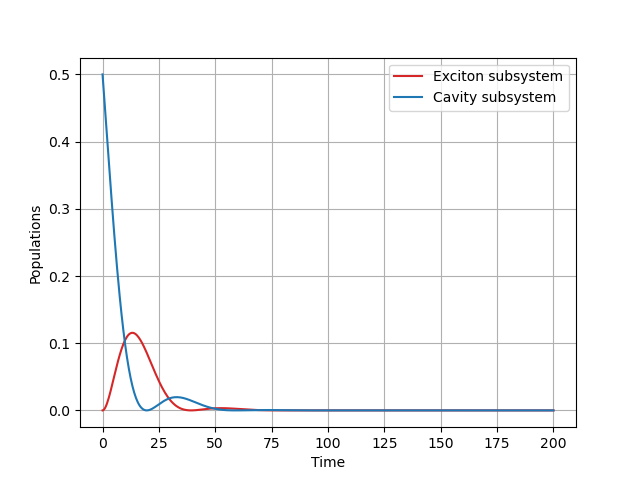
\includegraphics[width=\linewidth]{Research Project/Code/results/JCM/OQS_Pop_Both_eg.png}
        \caption{}
        \label{fig:JCM_OQS_Pop_Both_eg}
    \end{subfigure}
    \hfill

    \caption{}
    \label{fig:JCM_OQS_Pop_eg}
\end{figure}

Figure \ref{fig:JCM_OQS_Pop_eg} shows that the populations decay at the same rate as with the previous initial condition in figure \ref{fig:JCM_OQS_Pop} for all decay channel types. This is expected, as we use the same decay parameters ($\gamma= \gamma_{\scriptscriptstyle \text{th}} = 0.01$) as with the previous initial condition. The only difference is that the population probability for the excited atomic state is 0.5 initially, which is in line with our initial state being an equal superposition of the $|e\rangle$ and $|g\rangle$ atomic states coupled to the $|n=0\rangle$ fock state of the cavity. \\
\\
For coherence, we observe the same features in figure \ref{fig:JCM_OQS_Coh_eg} as we saw with the closed evolution coherence  -- the $|g,0\rangle$ contribution adds an off--diagonal term to our full system, thus creating a baseline level of coherence throughout the evolution, as can be seen by the total system's coherence being greater than 0. Other than this, the decoherence of our system behaves as expected, with the decay timescales matching the population decay timescales (which we also observed in our first initial state), and the coherences being present (and thus decaying) in our subsystems. 


\begin{figure}[H]
    \centering
    \begin{subfigure}{0.45\textwidth}
        \centering
        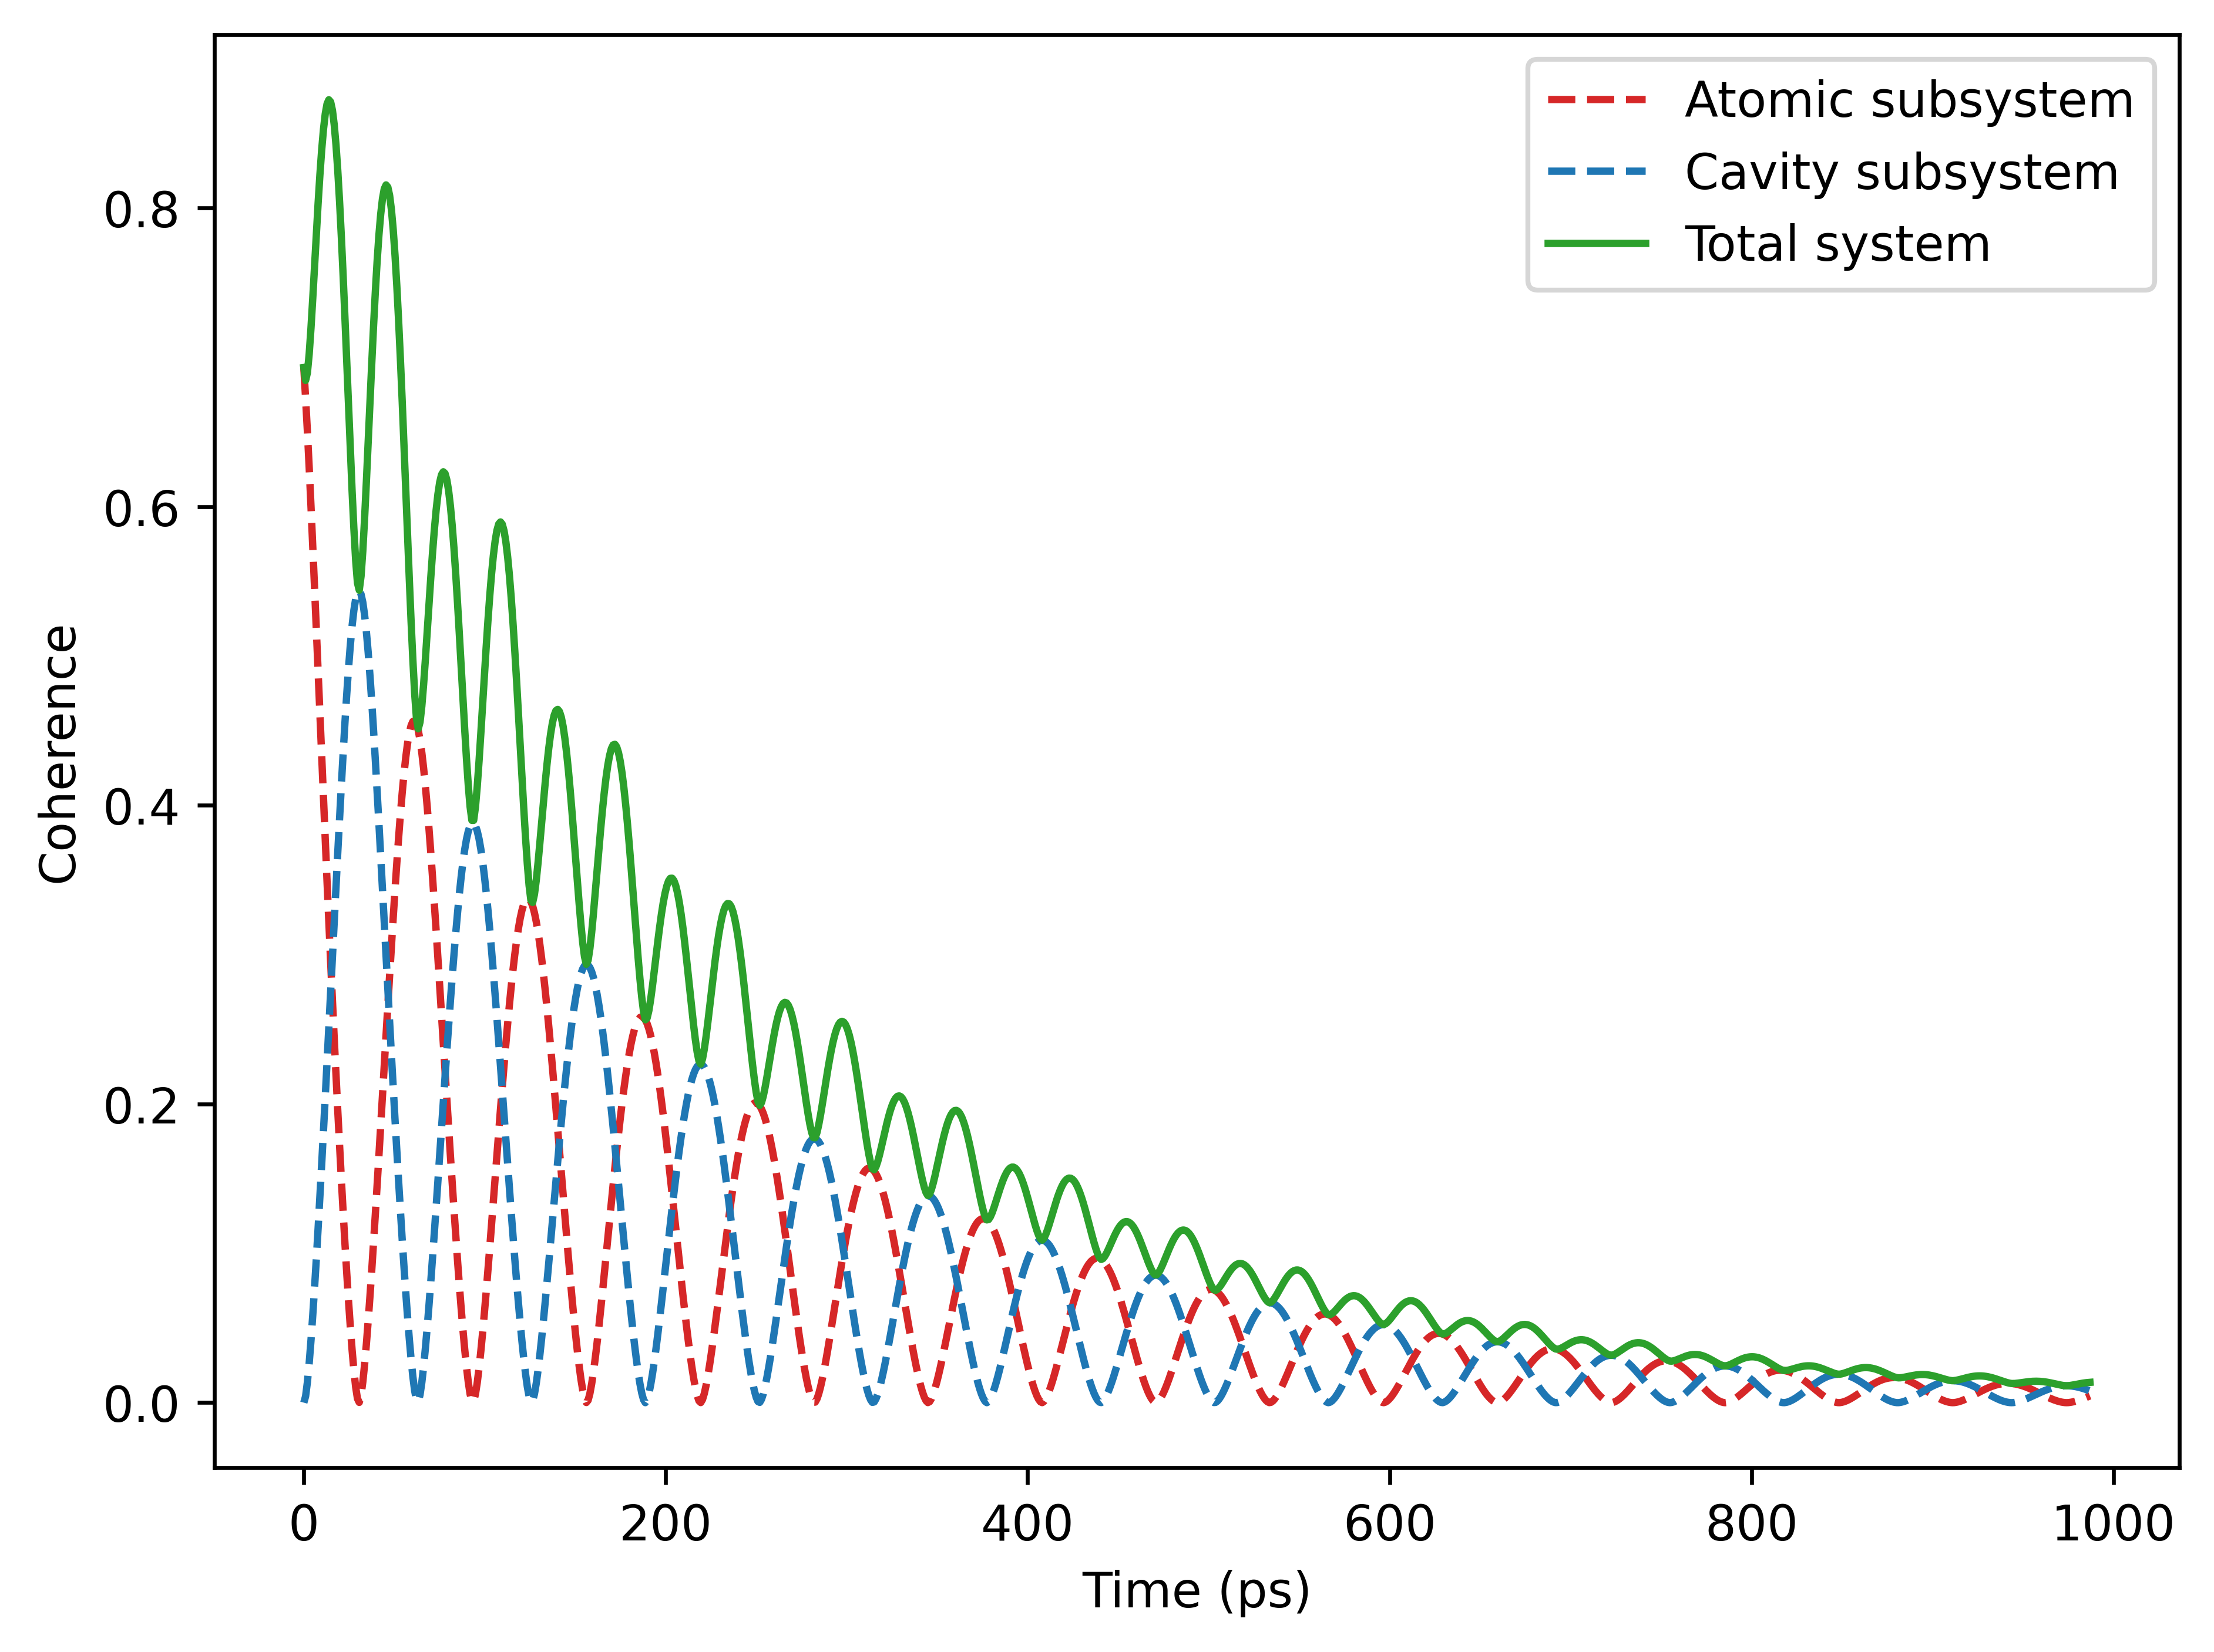
\includegraphics[width=0.85\linewidth]{Research Project/Code/results/JCM/OQS_Coh_Spont_eg.png}
        \caption{}
        \label{fig:JCM_OQS_Coh_Spont_eg}
    \end{subfigure}
    \hfill
    \begin{subfigure}{0.45\textwidth}
        \centering
        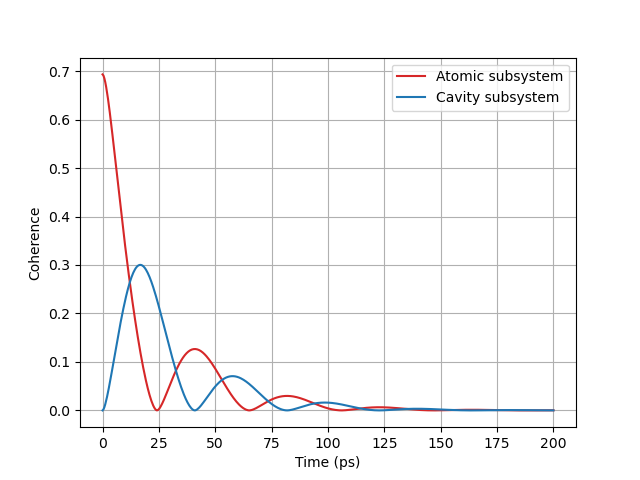
\includegraphics[width=0.85\linewidth]{Research Project/Code/results/JCM/OQS_Coh_Therm_eg.png}
        \caption{}
        \label{fig:JCM_OQS_Coh_Therm_eg}
    \end{subfigure}
    
    \vspace{0.5cm}
    
    \begin{subfigure}{0.45\textwidth}
        \centering
        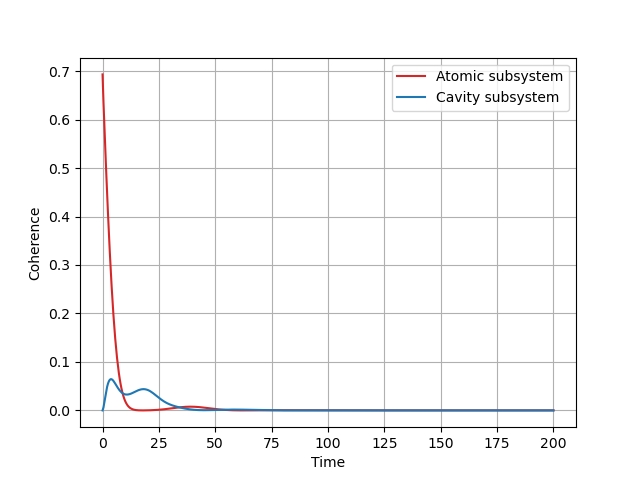
\includegraphics[width=0.85\linewidth]{Research Project/Code/results/JCM/OQS_Coh_Both_eg.png}
        \caption{}
        \label{fig:JCM_OQS_Coh_Both_eg}
    \end{subfigure}
    \hfill
    \caption{}
    \label{fig:JCM_OQS_Coh_eg}
\end{figure}


\begin{figure}[H]
    \centering
    \begin{subfigure}{0.45\textwidth}
        \centering
        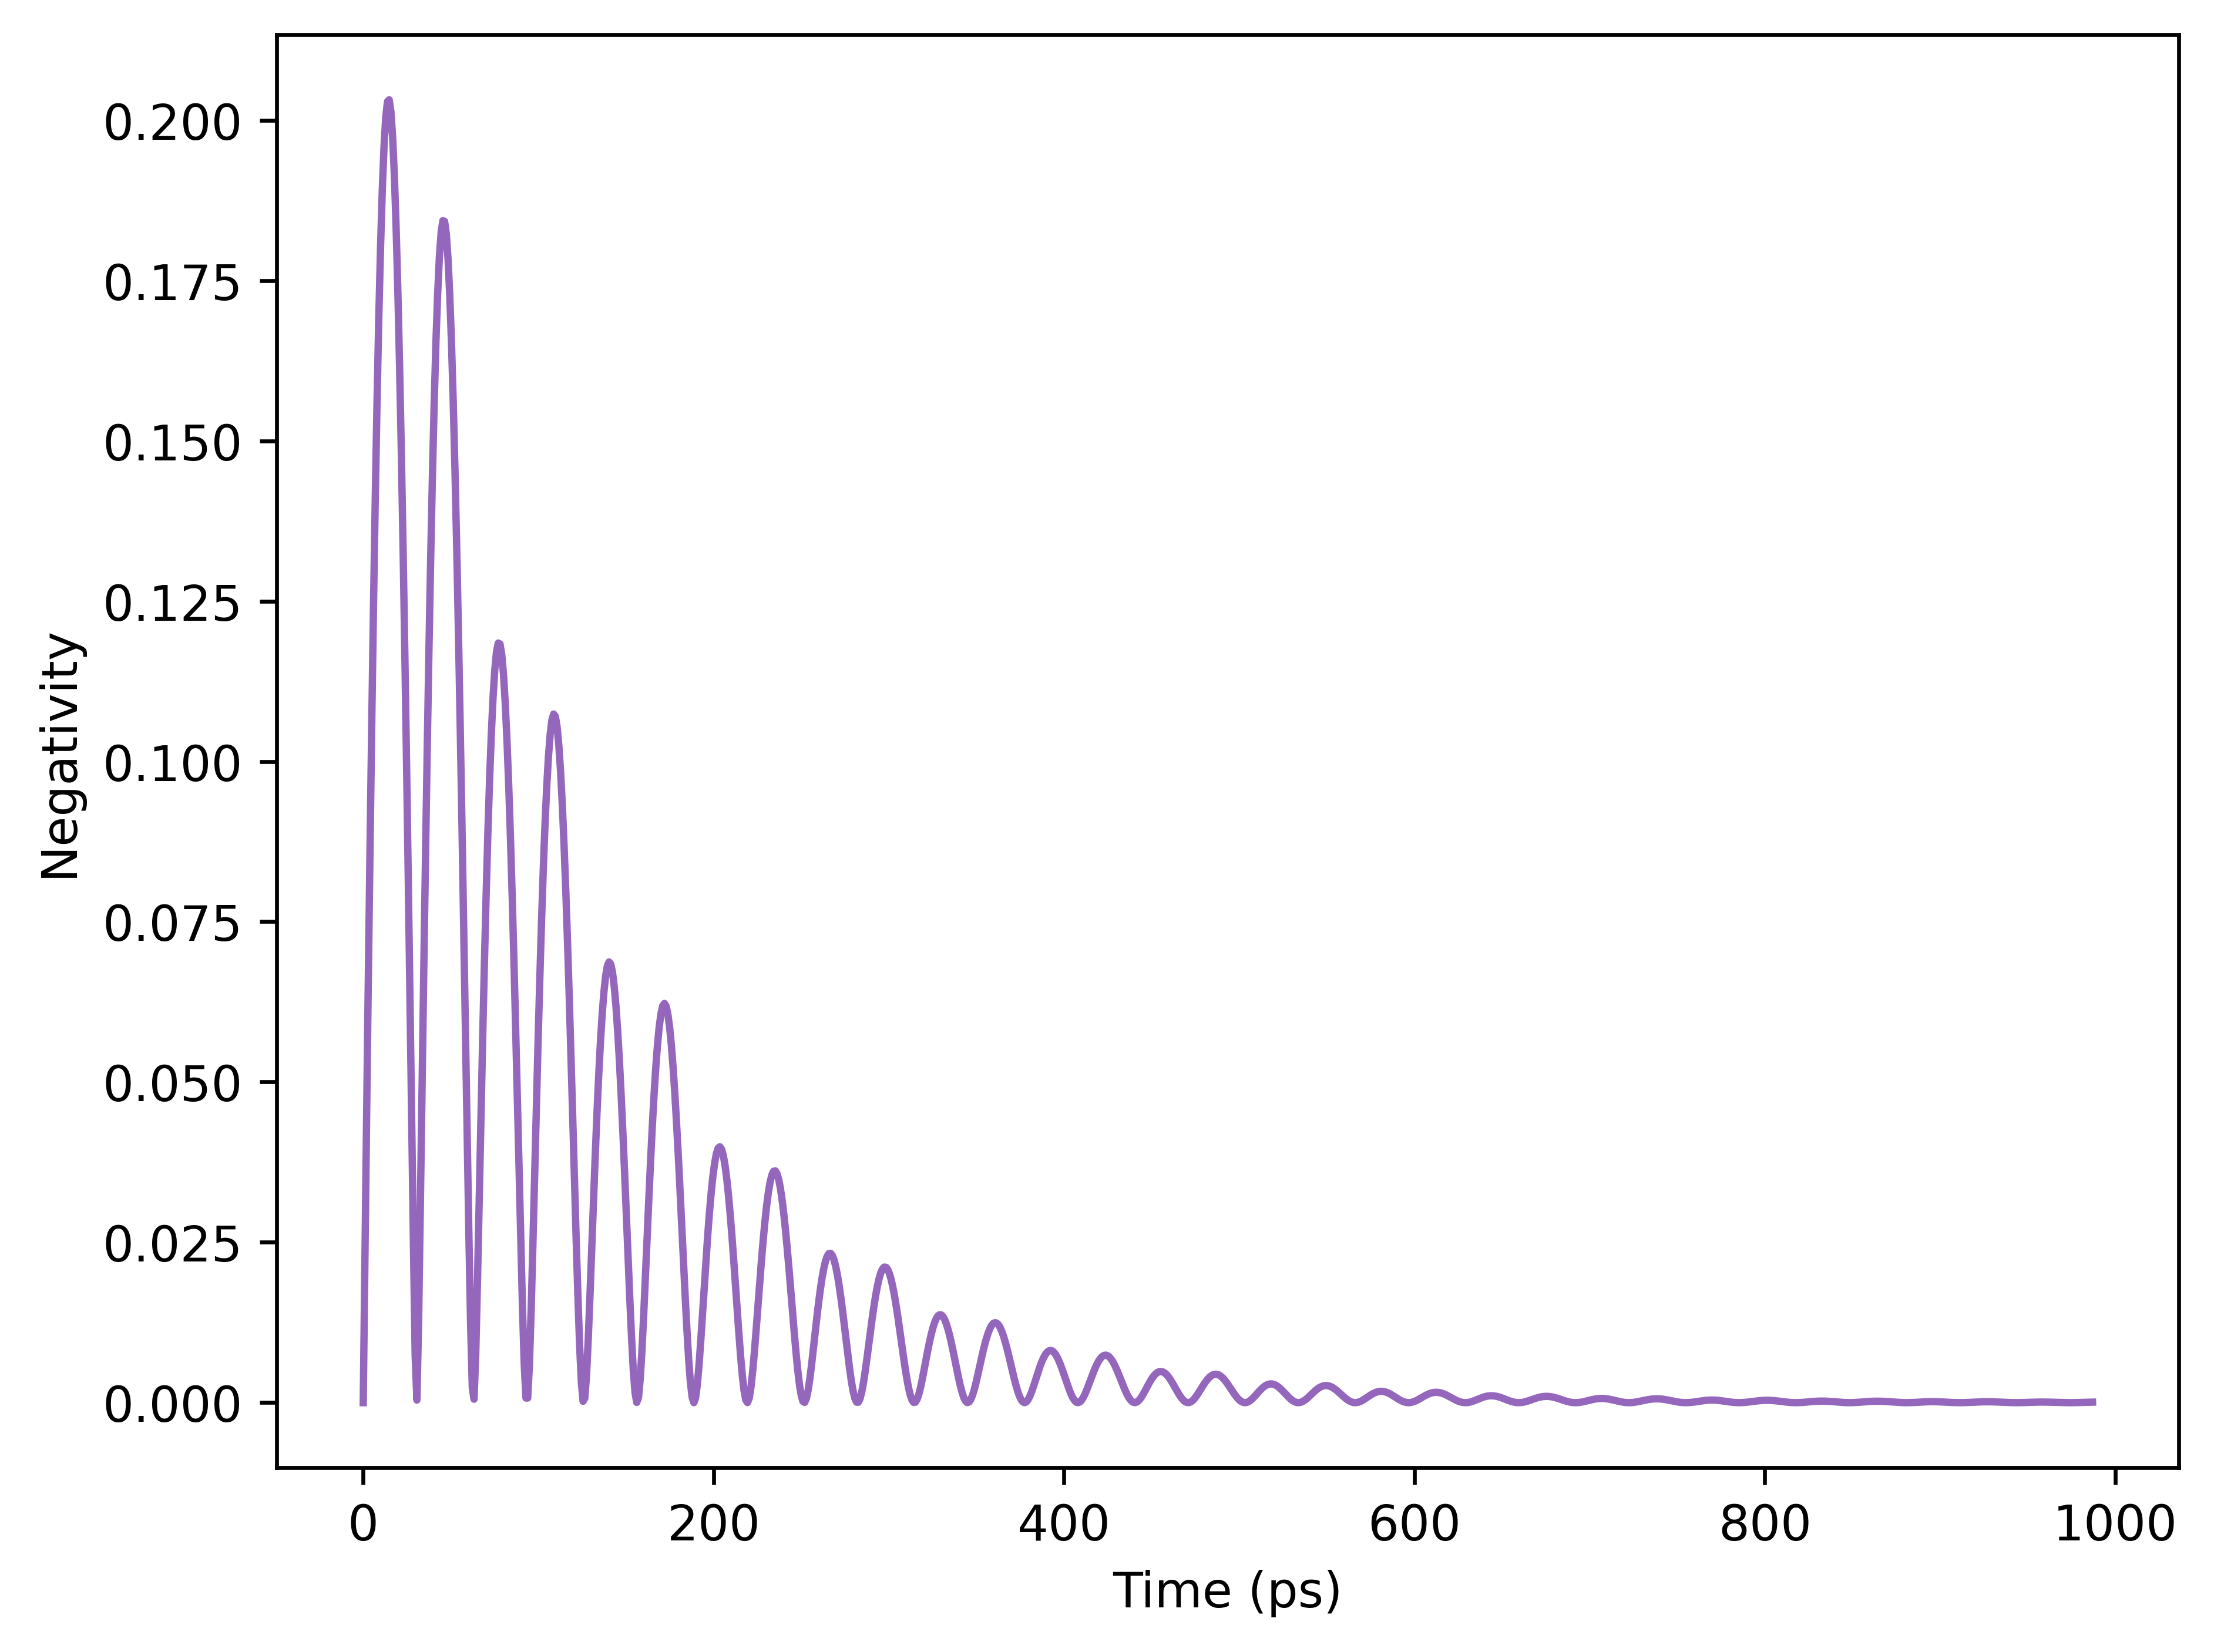
\includegraphics[width=0.85\linewidth]{Research Project/Code/results/JCM/OQS_Neg_Spont_eg.png}
        \caption{}
        \label{fig:jcm_cqs_expt_eg}
    \end{subfigure}
    \hfill
    \begin{subfigure}{0.45\textwidth}
        \centering
        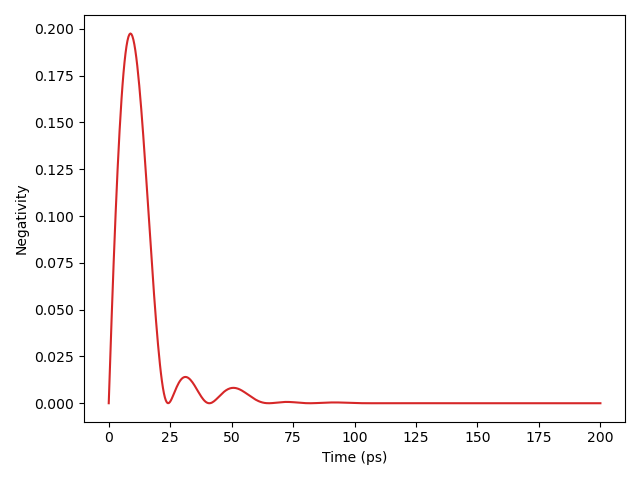
\includegraphics[width=0.85\linewidth]{Research Project/Code/results/JCM/OQS_Neg_Therm_eg.png}
        \caption{}
        \label{fig:jcm_cqs_vne_eg}
    \end{subfigure}
    
    \vspace{0.5cm}
    
    \begin{subfigure}{0.45\textwidth}
        \centering
        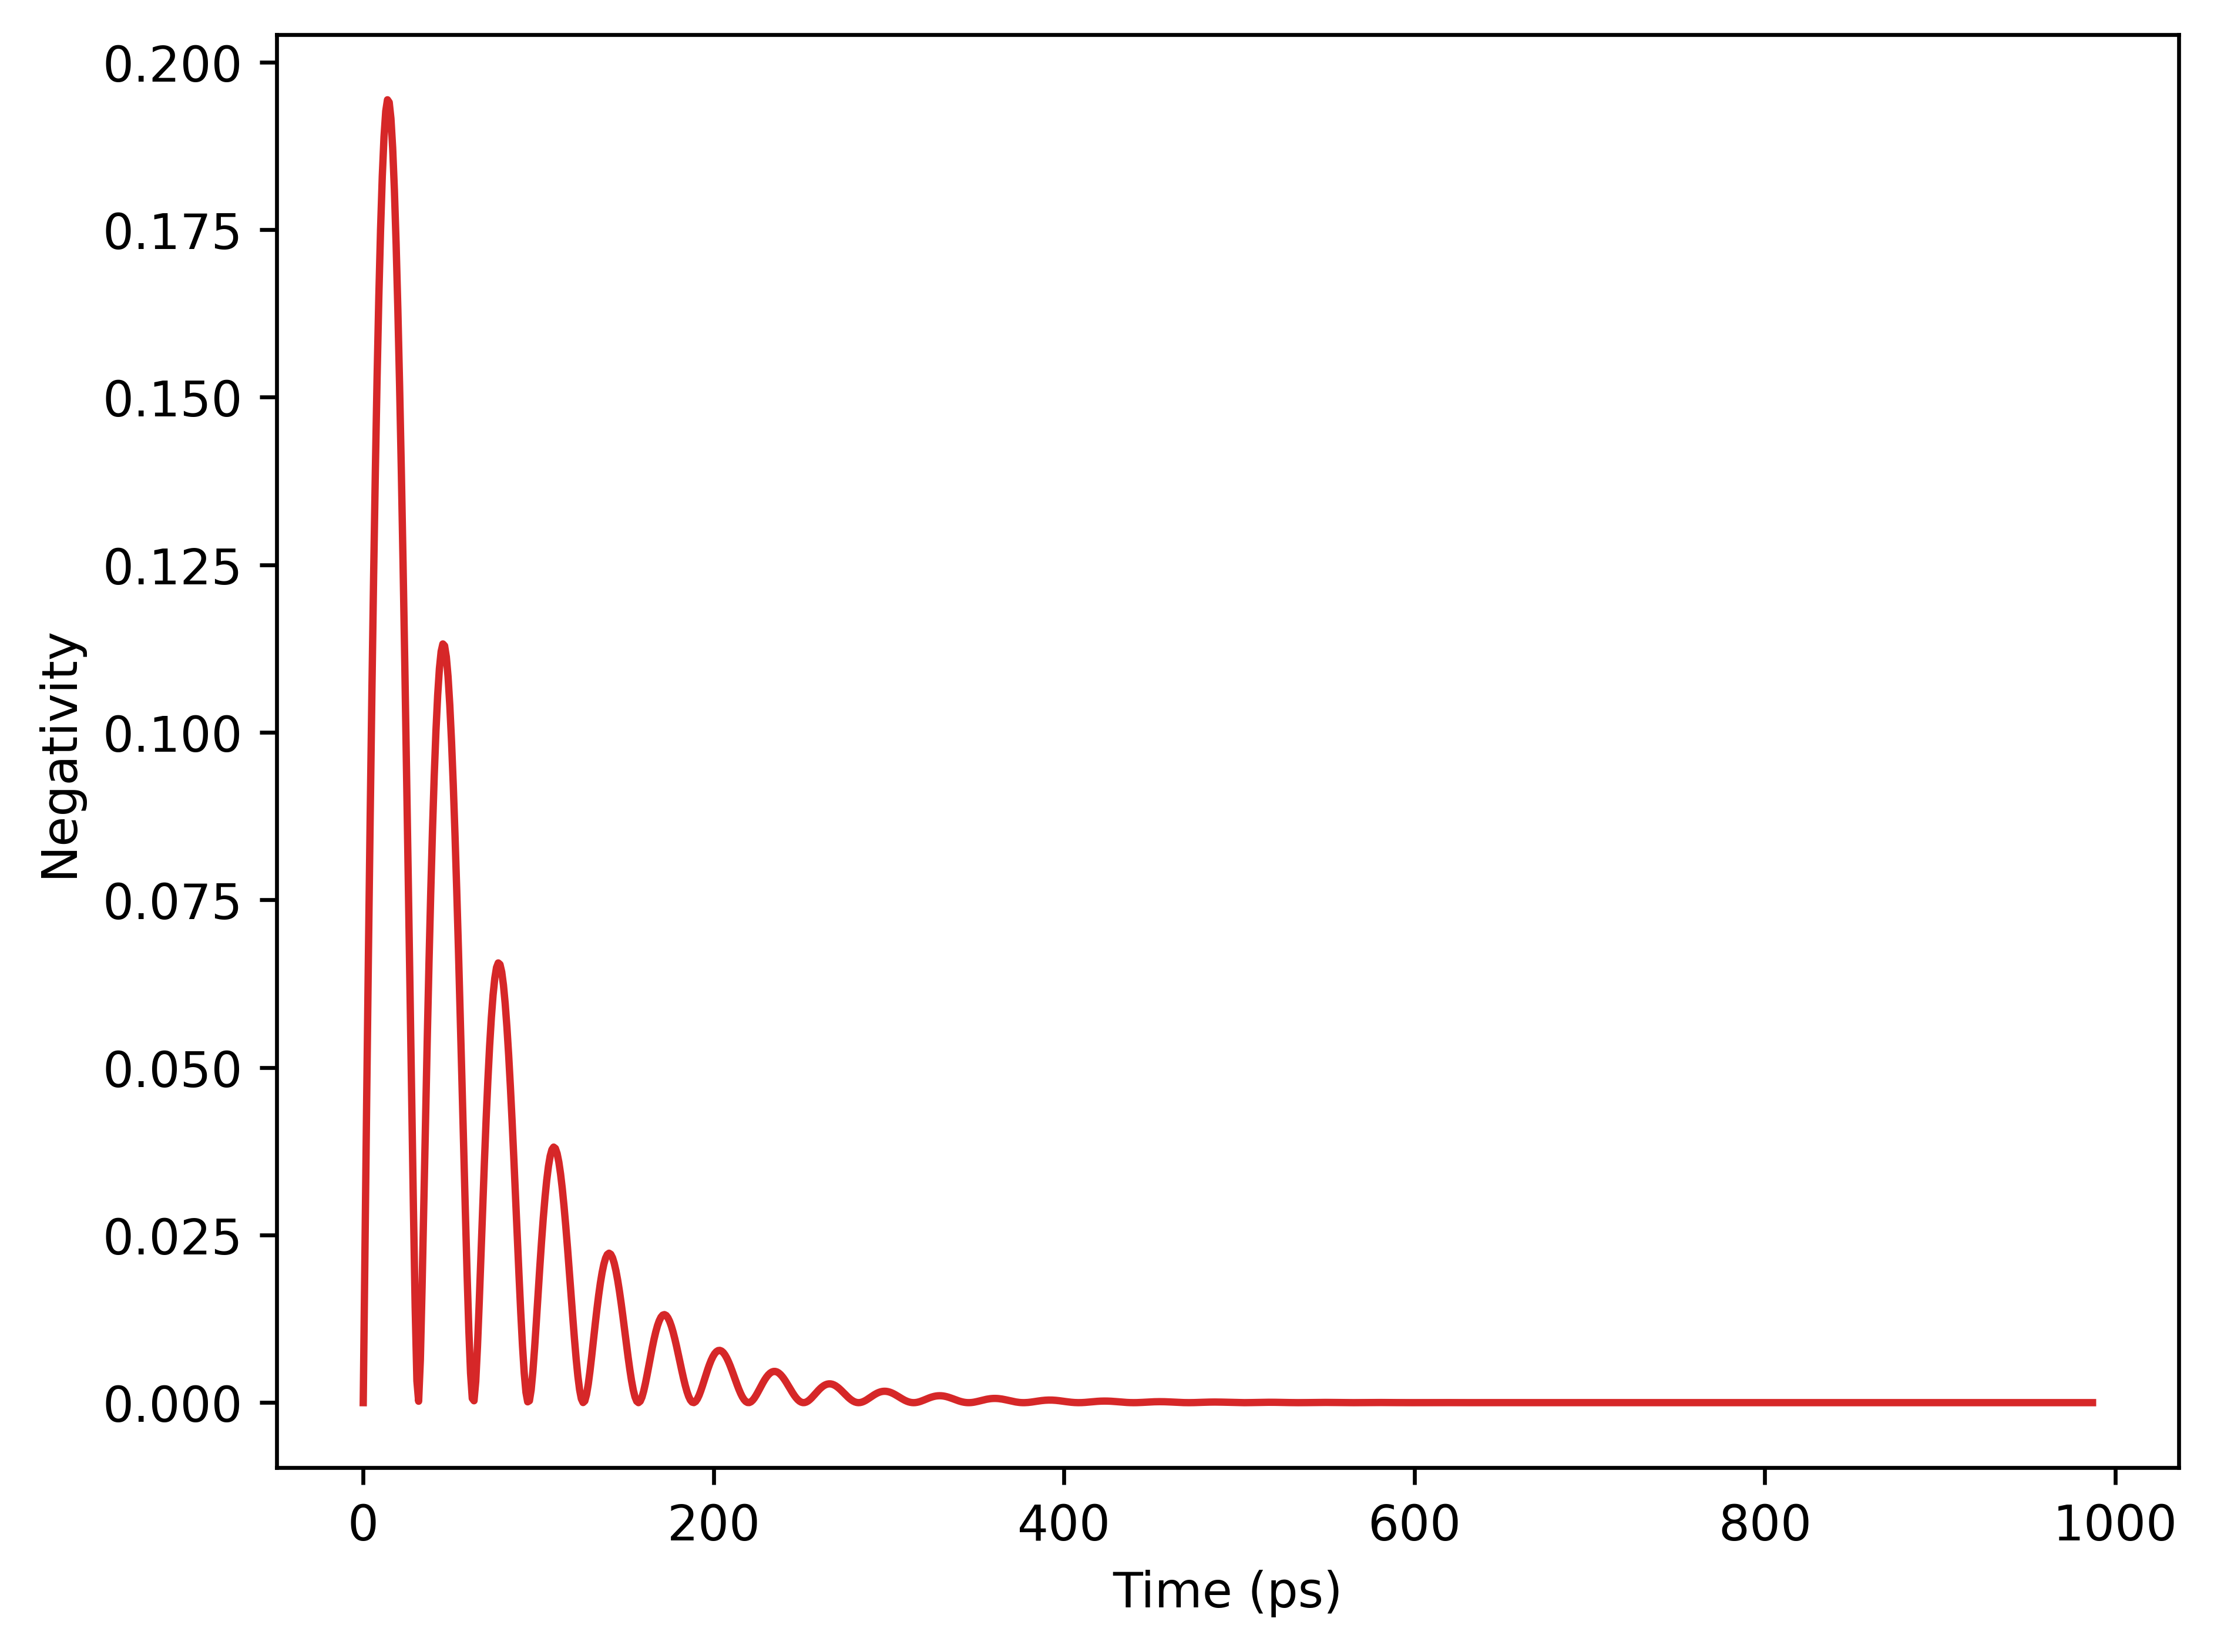
\includegraphics[width=0.85\linewidth]{Research Project/Code/results/JCM/OQS_Neg_Both_eg.png}
        \caption{}
        \label{fig:jcm_cqs_coh_eg}
    \end{subfigure}
    \hfill
    \caption{}
\end{figure}


\subsection{Population, Entanglement and Coherence of the Exciton--Vibration Model}
\subsubsection{Closed Evolution}

\begin{figure}[H]
    \centering
    \begin{subfigure}{0.49\textwidth}
        \centering
        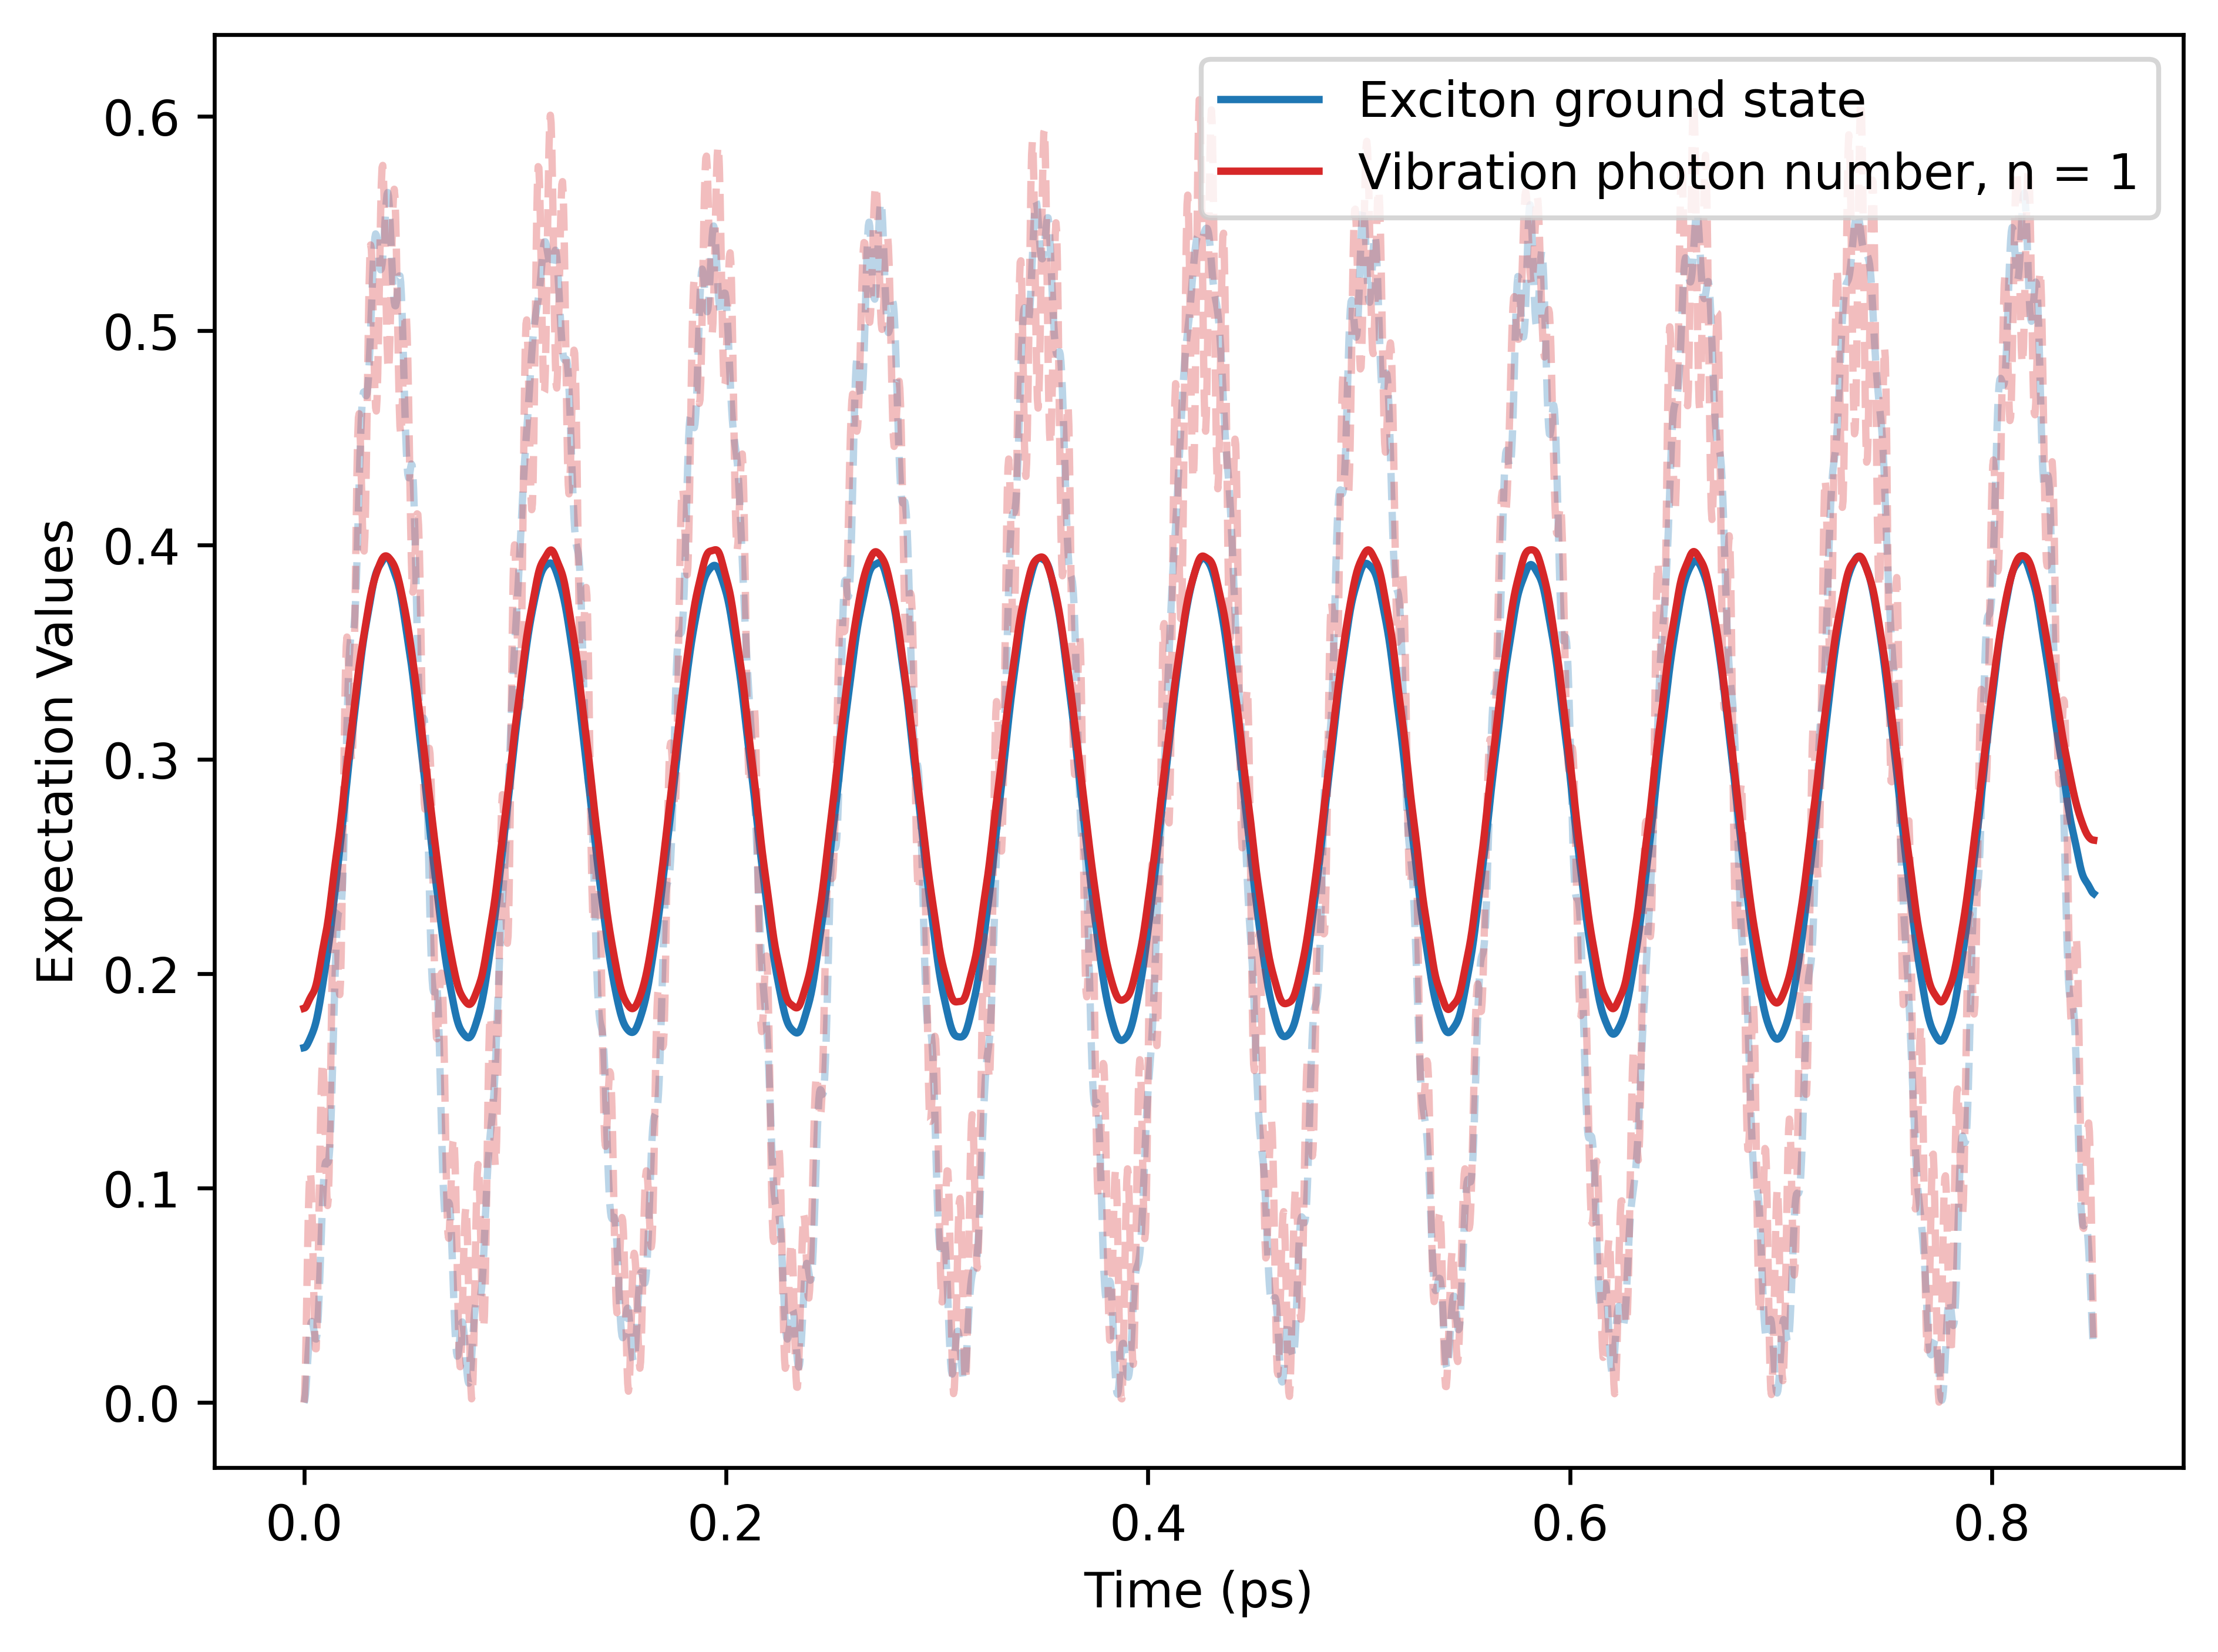
\includegraphics[width=\linewidth]{Research Project/Code/results/ExVib/Closed/Envelope/pops_ground.png}
        \caption{}
        \label{fig:EVM_CQS_Pop_env}
    \end{subfigure}
    \hfill
    \begin{subfigure}{0.49\textwidth}
        \centering
        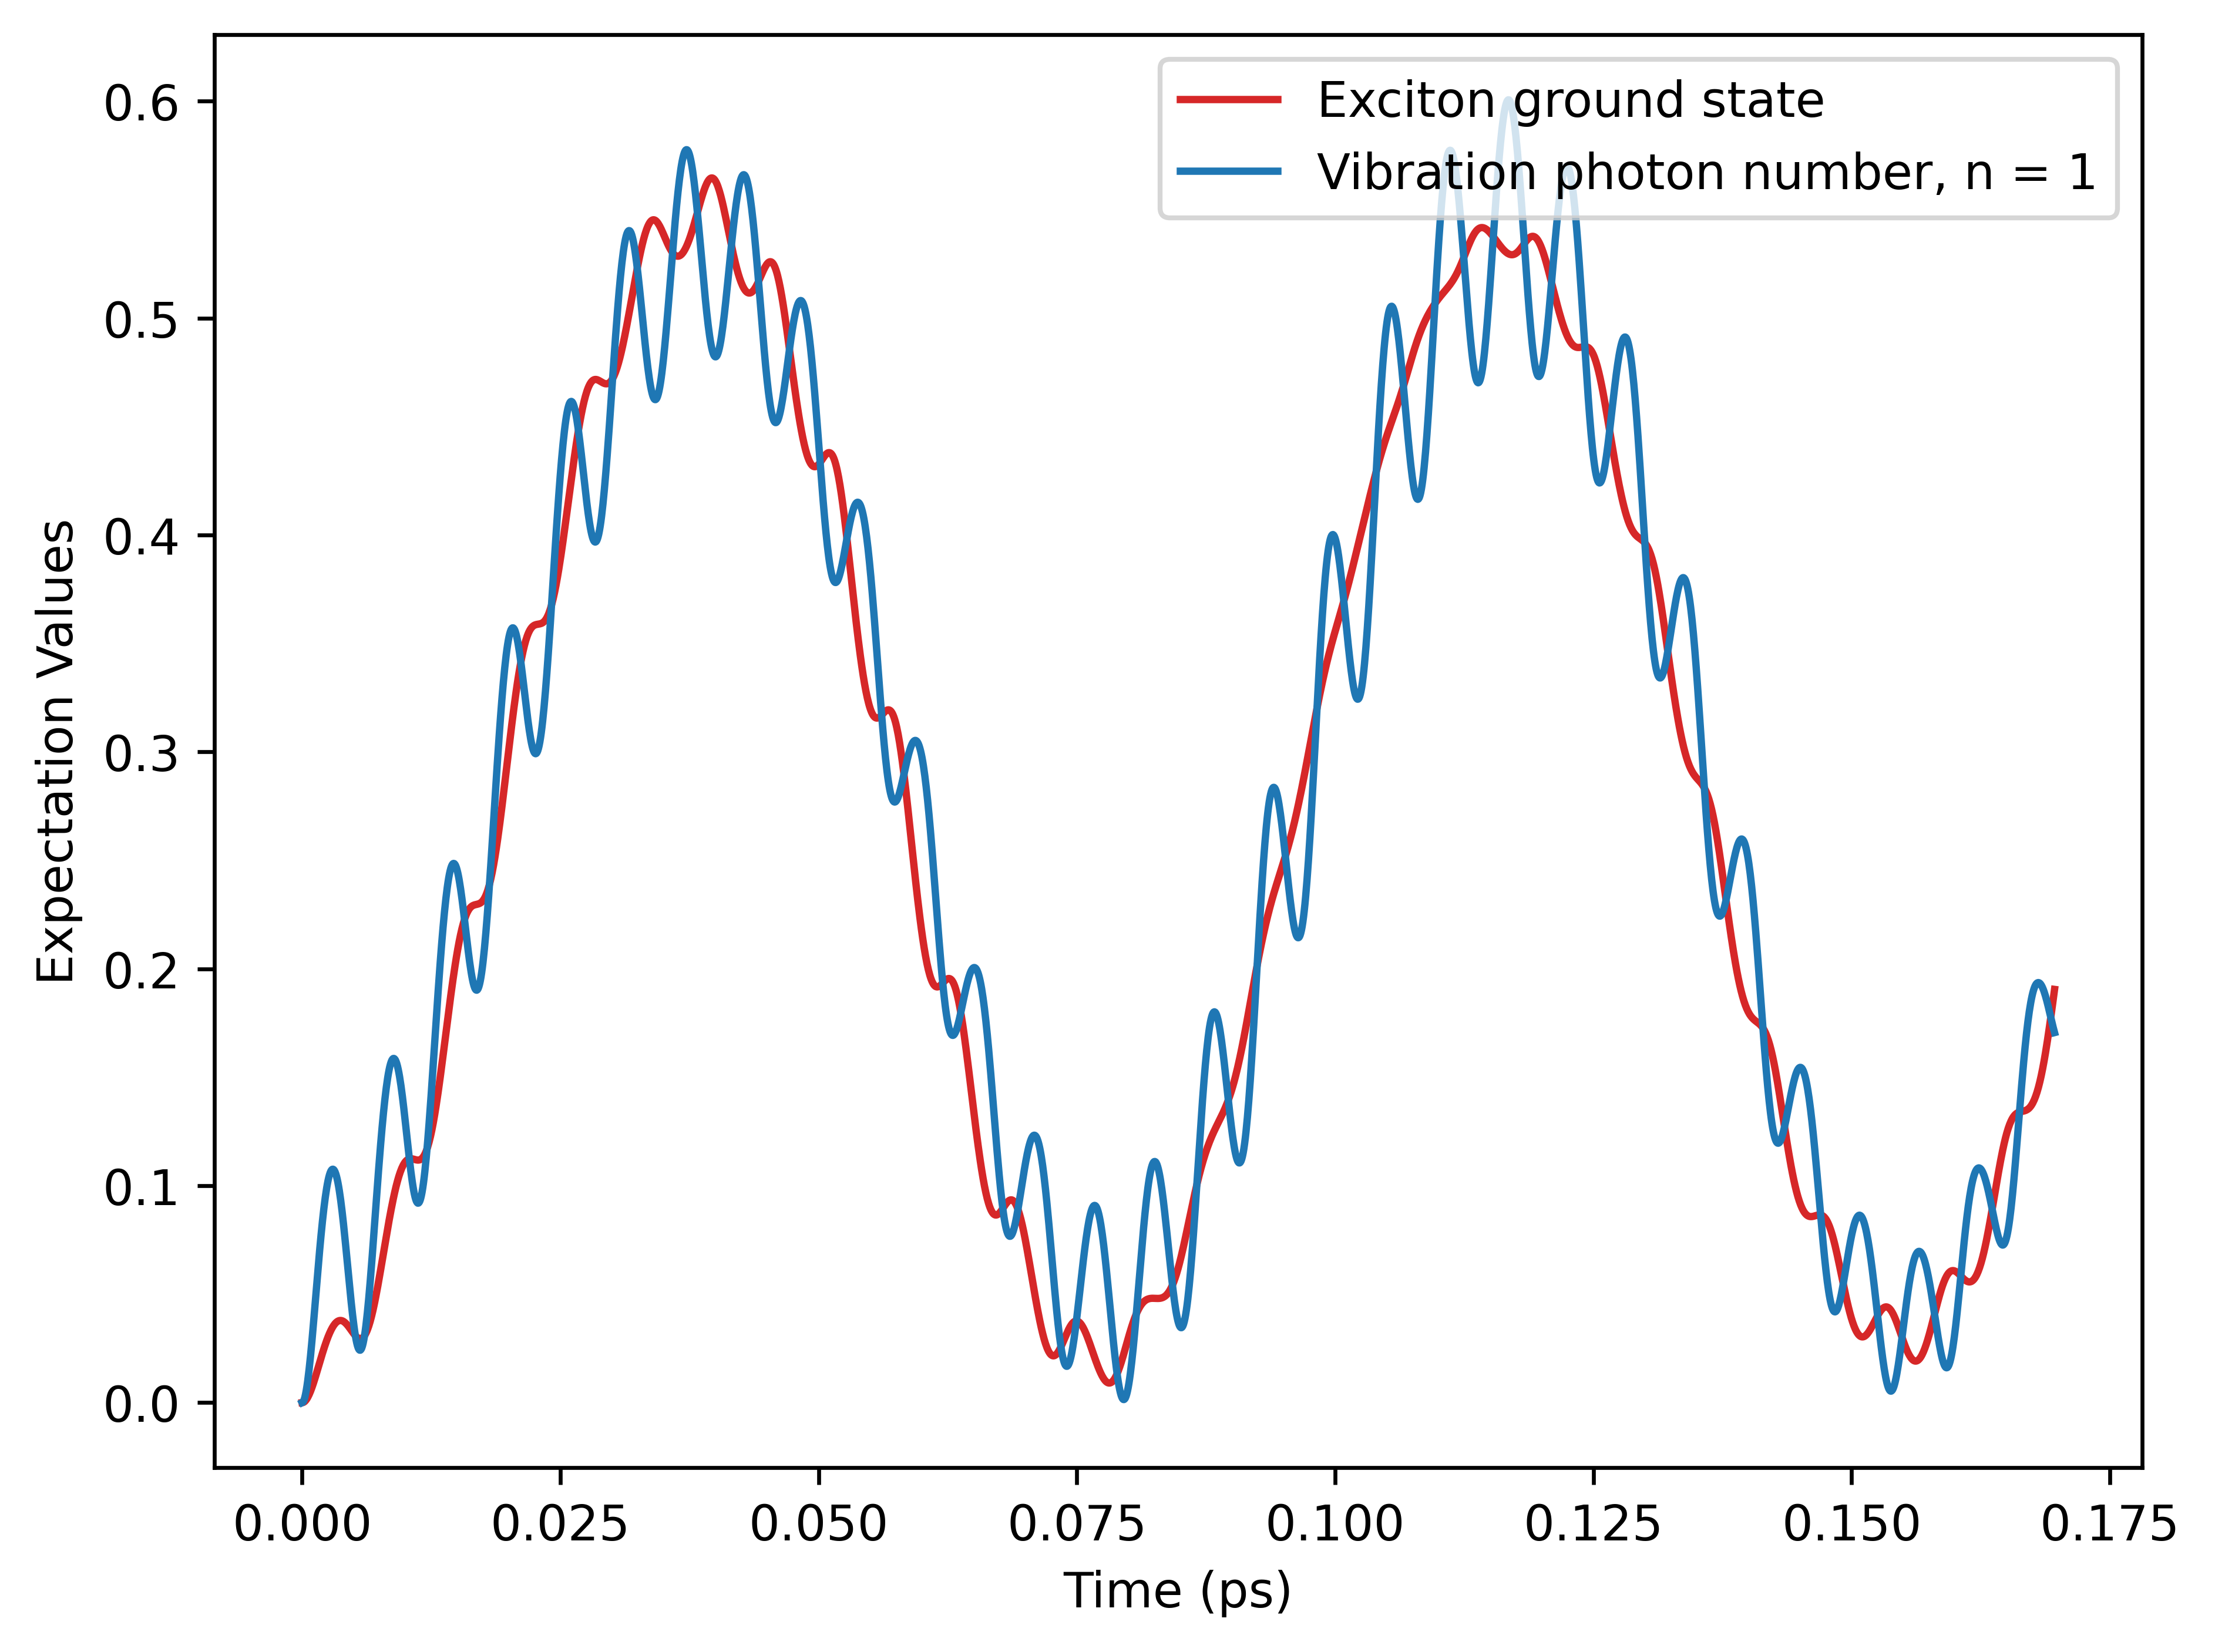
\includegraphics[width=\linewidth]{Research Project/Code/results/ExVib/Closed/Fast/pops_ground.png}
        \caption{}
        \label{fig:EVM_CQS_Pop_fast}
    \end{subfigure}
    
    \caption{}
    \label{fig:EVM_CQS_Pops}
\end{figure}

\begin{figure}[H]
    \centering
    \begin{subfigure}{0.49\textwidth}
        \centering
        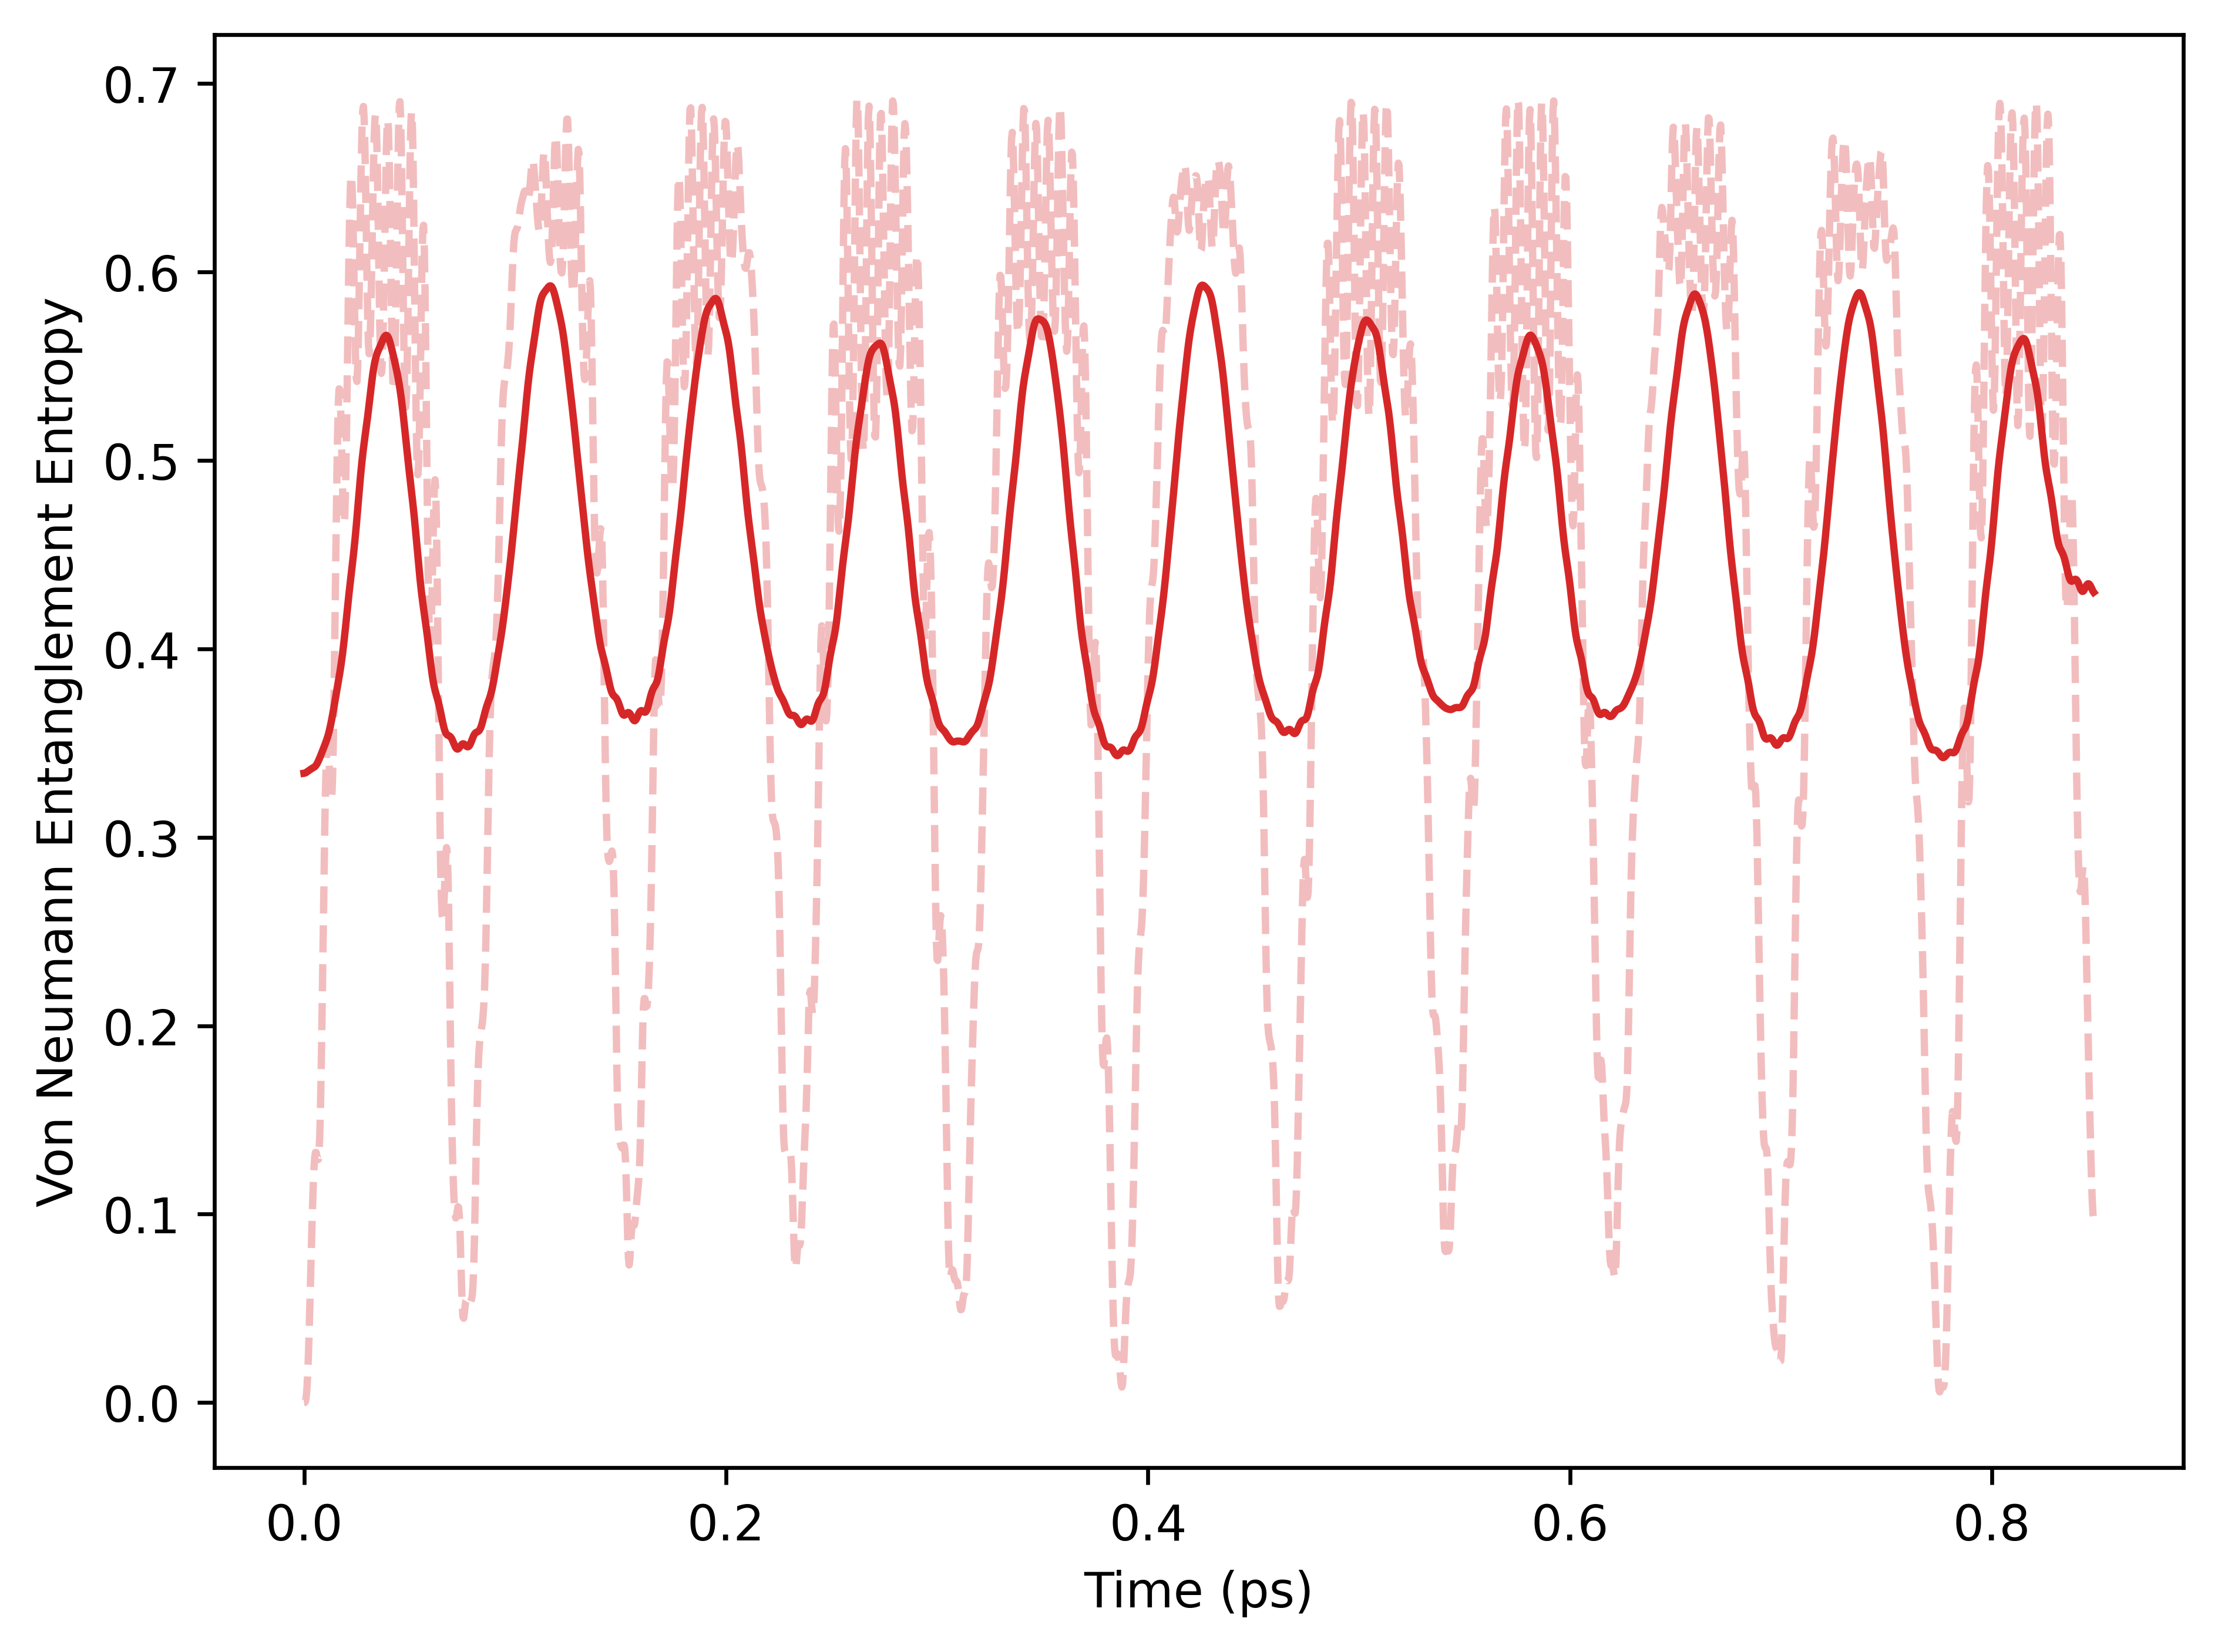
\includegraphics[width=\linewidth]{Research Project/Code/results/ExVib/Closed/Envelope/vne.png}
        \caption{}
        \label{fig:EVM_CQS_Ent_env}
    \end{subfigure}
    \hfill
    \begin{subfigure}{0.49\textwidth}
        \centering
        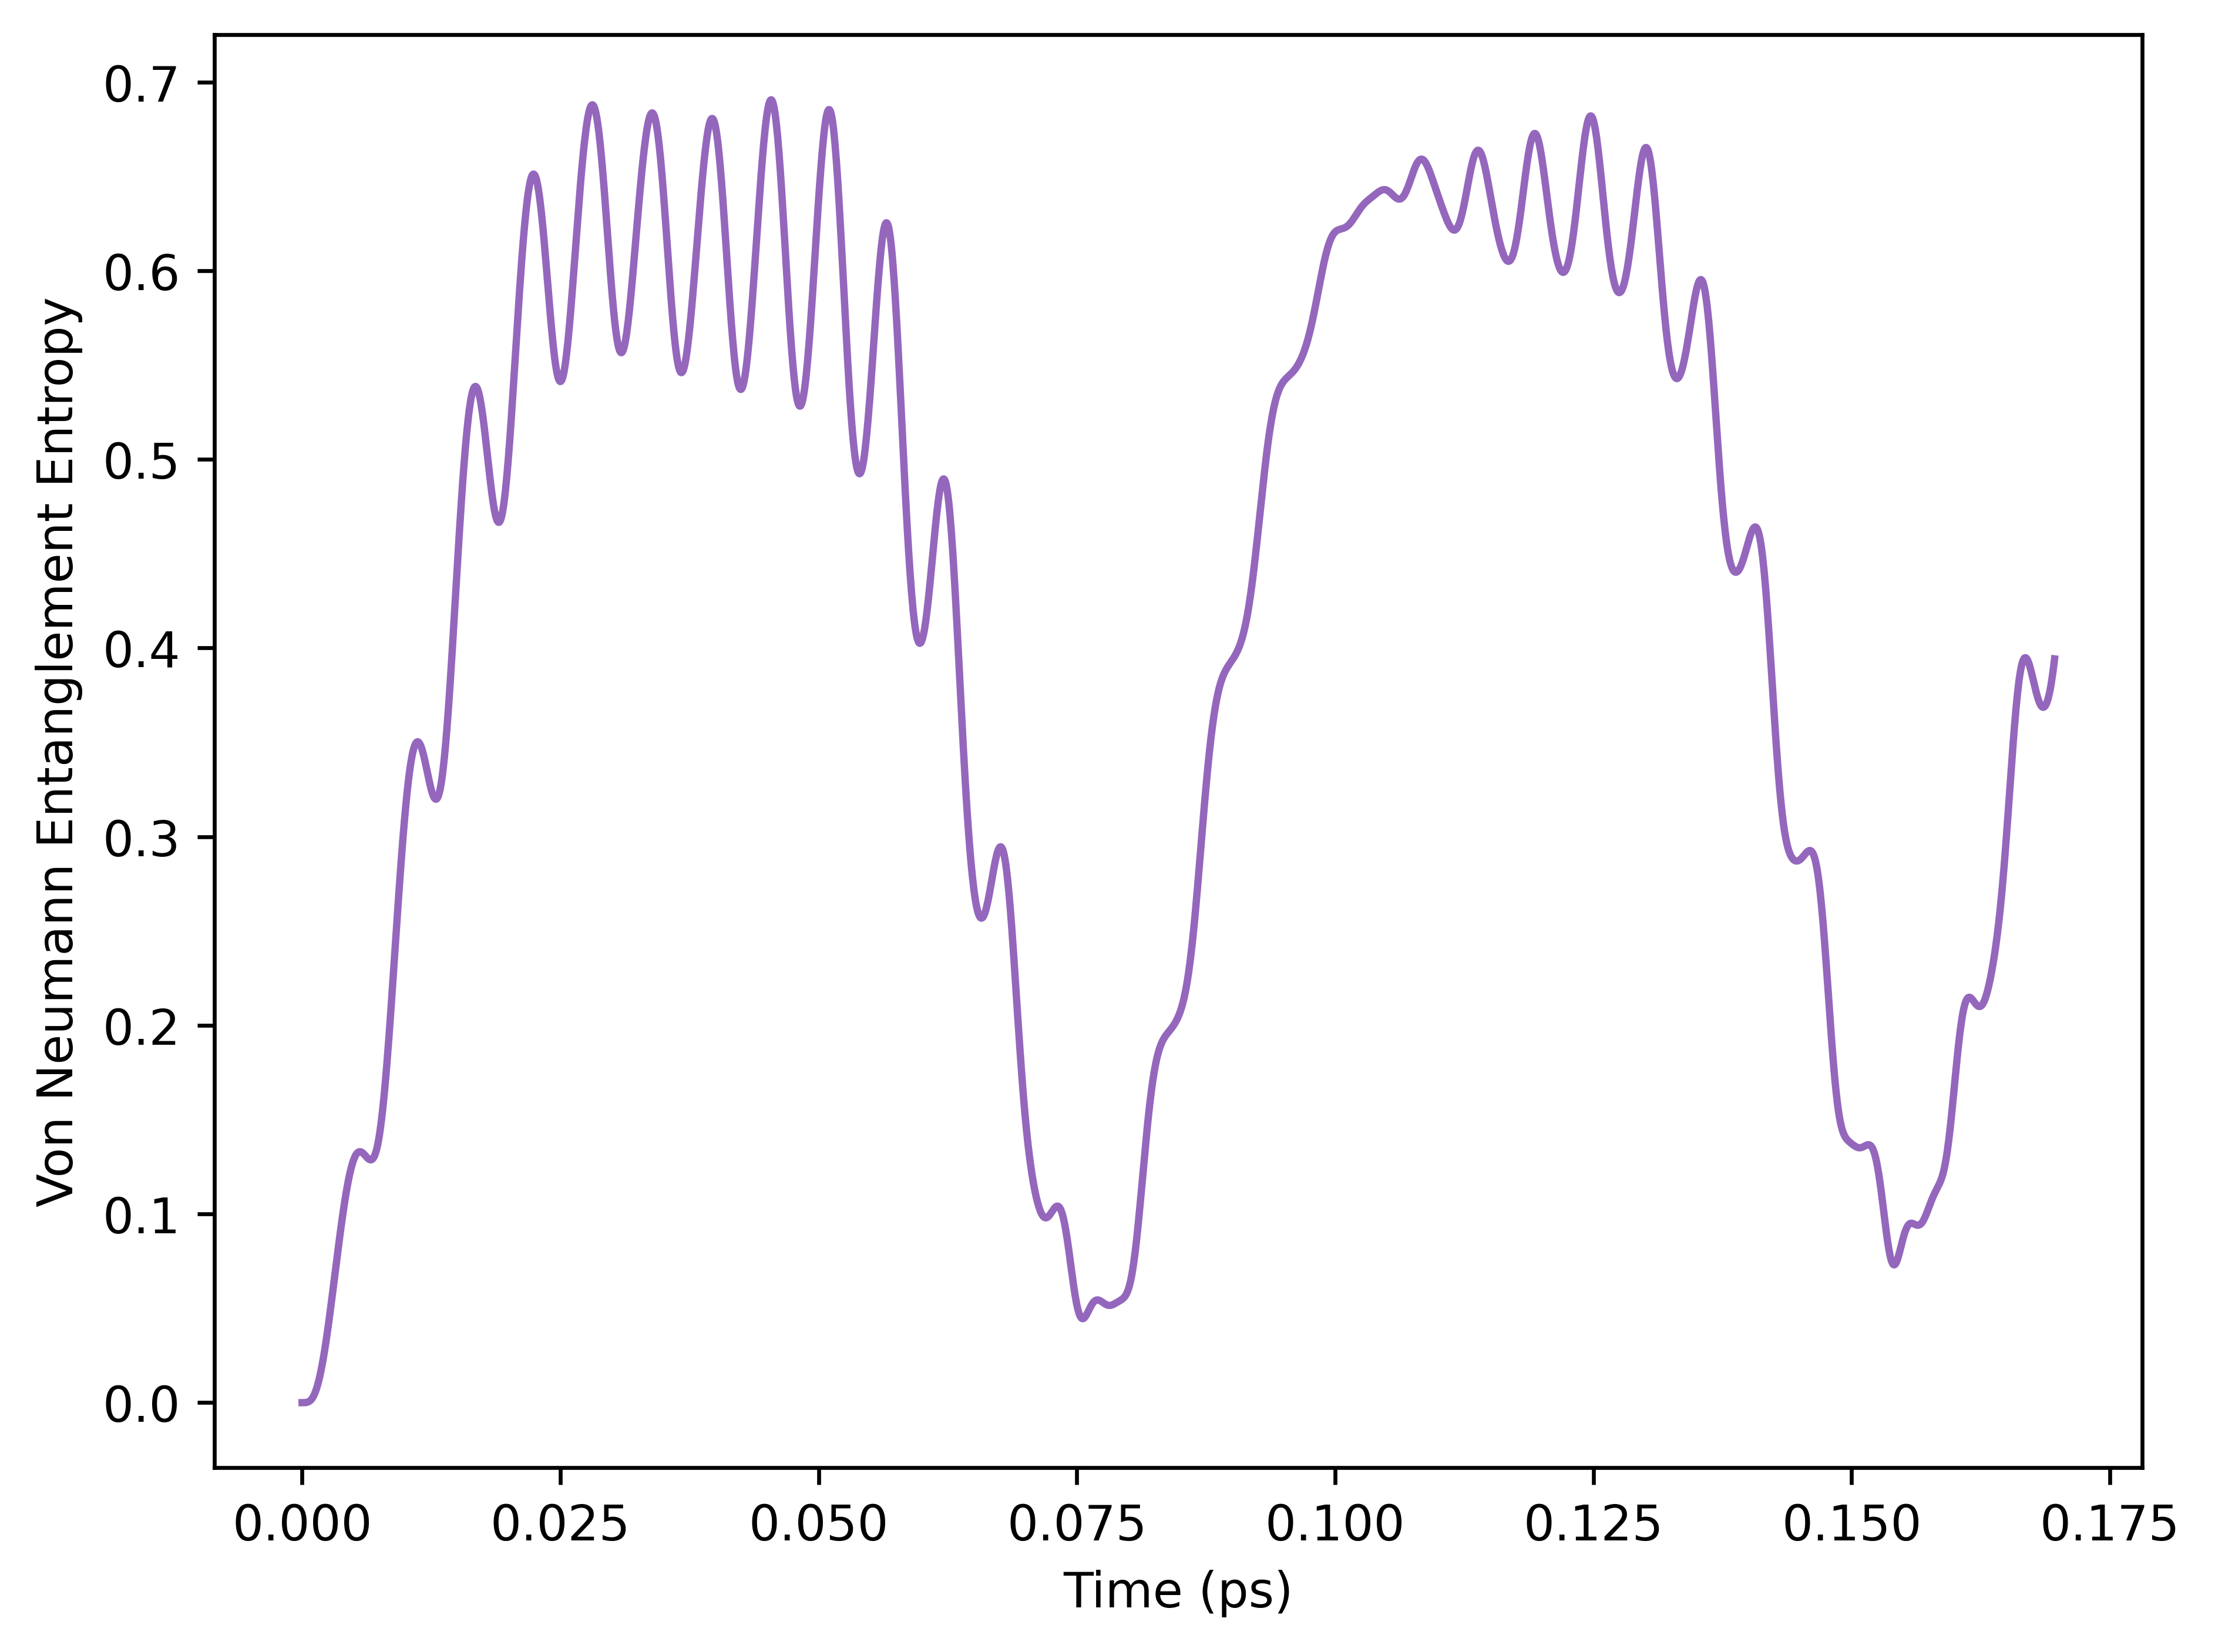
\includegraphics[width=\linewidth]{Research Project/Code/results/ExVib/Closed/Fast/vne.png}
        \caption{}
        \label{fig:EVM_CQS_Ent_fast}
    \end{subfigure}
    
    \caption{}
    \label{fig:EVM_CQS_Ent}
\end{figure}

\begin{figure}[H]
    \centering
    \begin{subfigure}{0.49\textwidth}
        \centering
        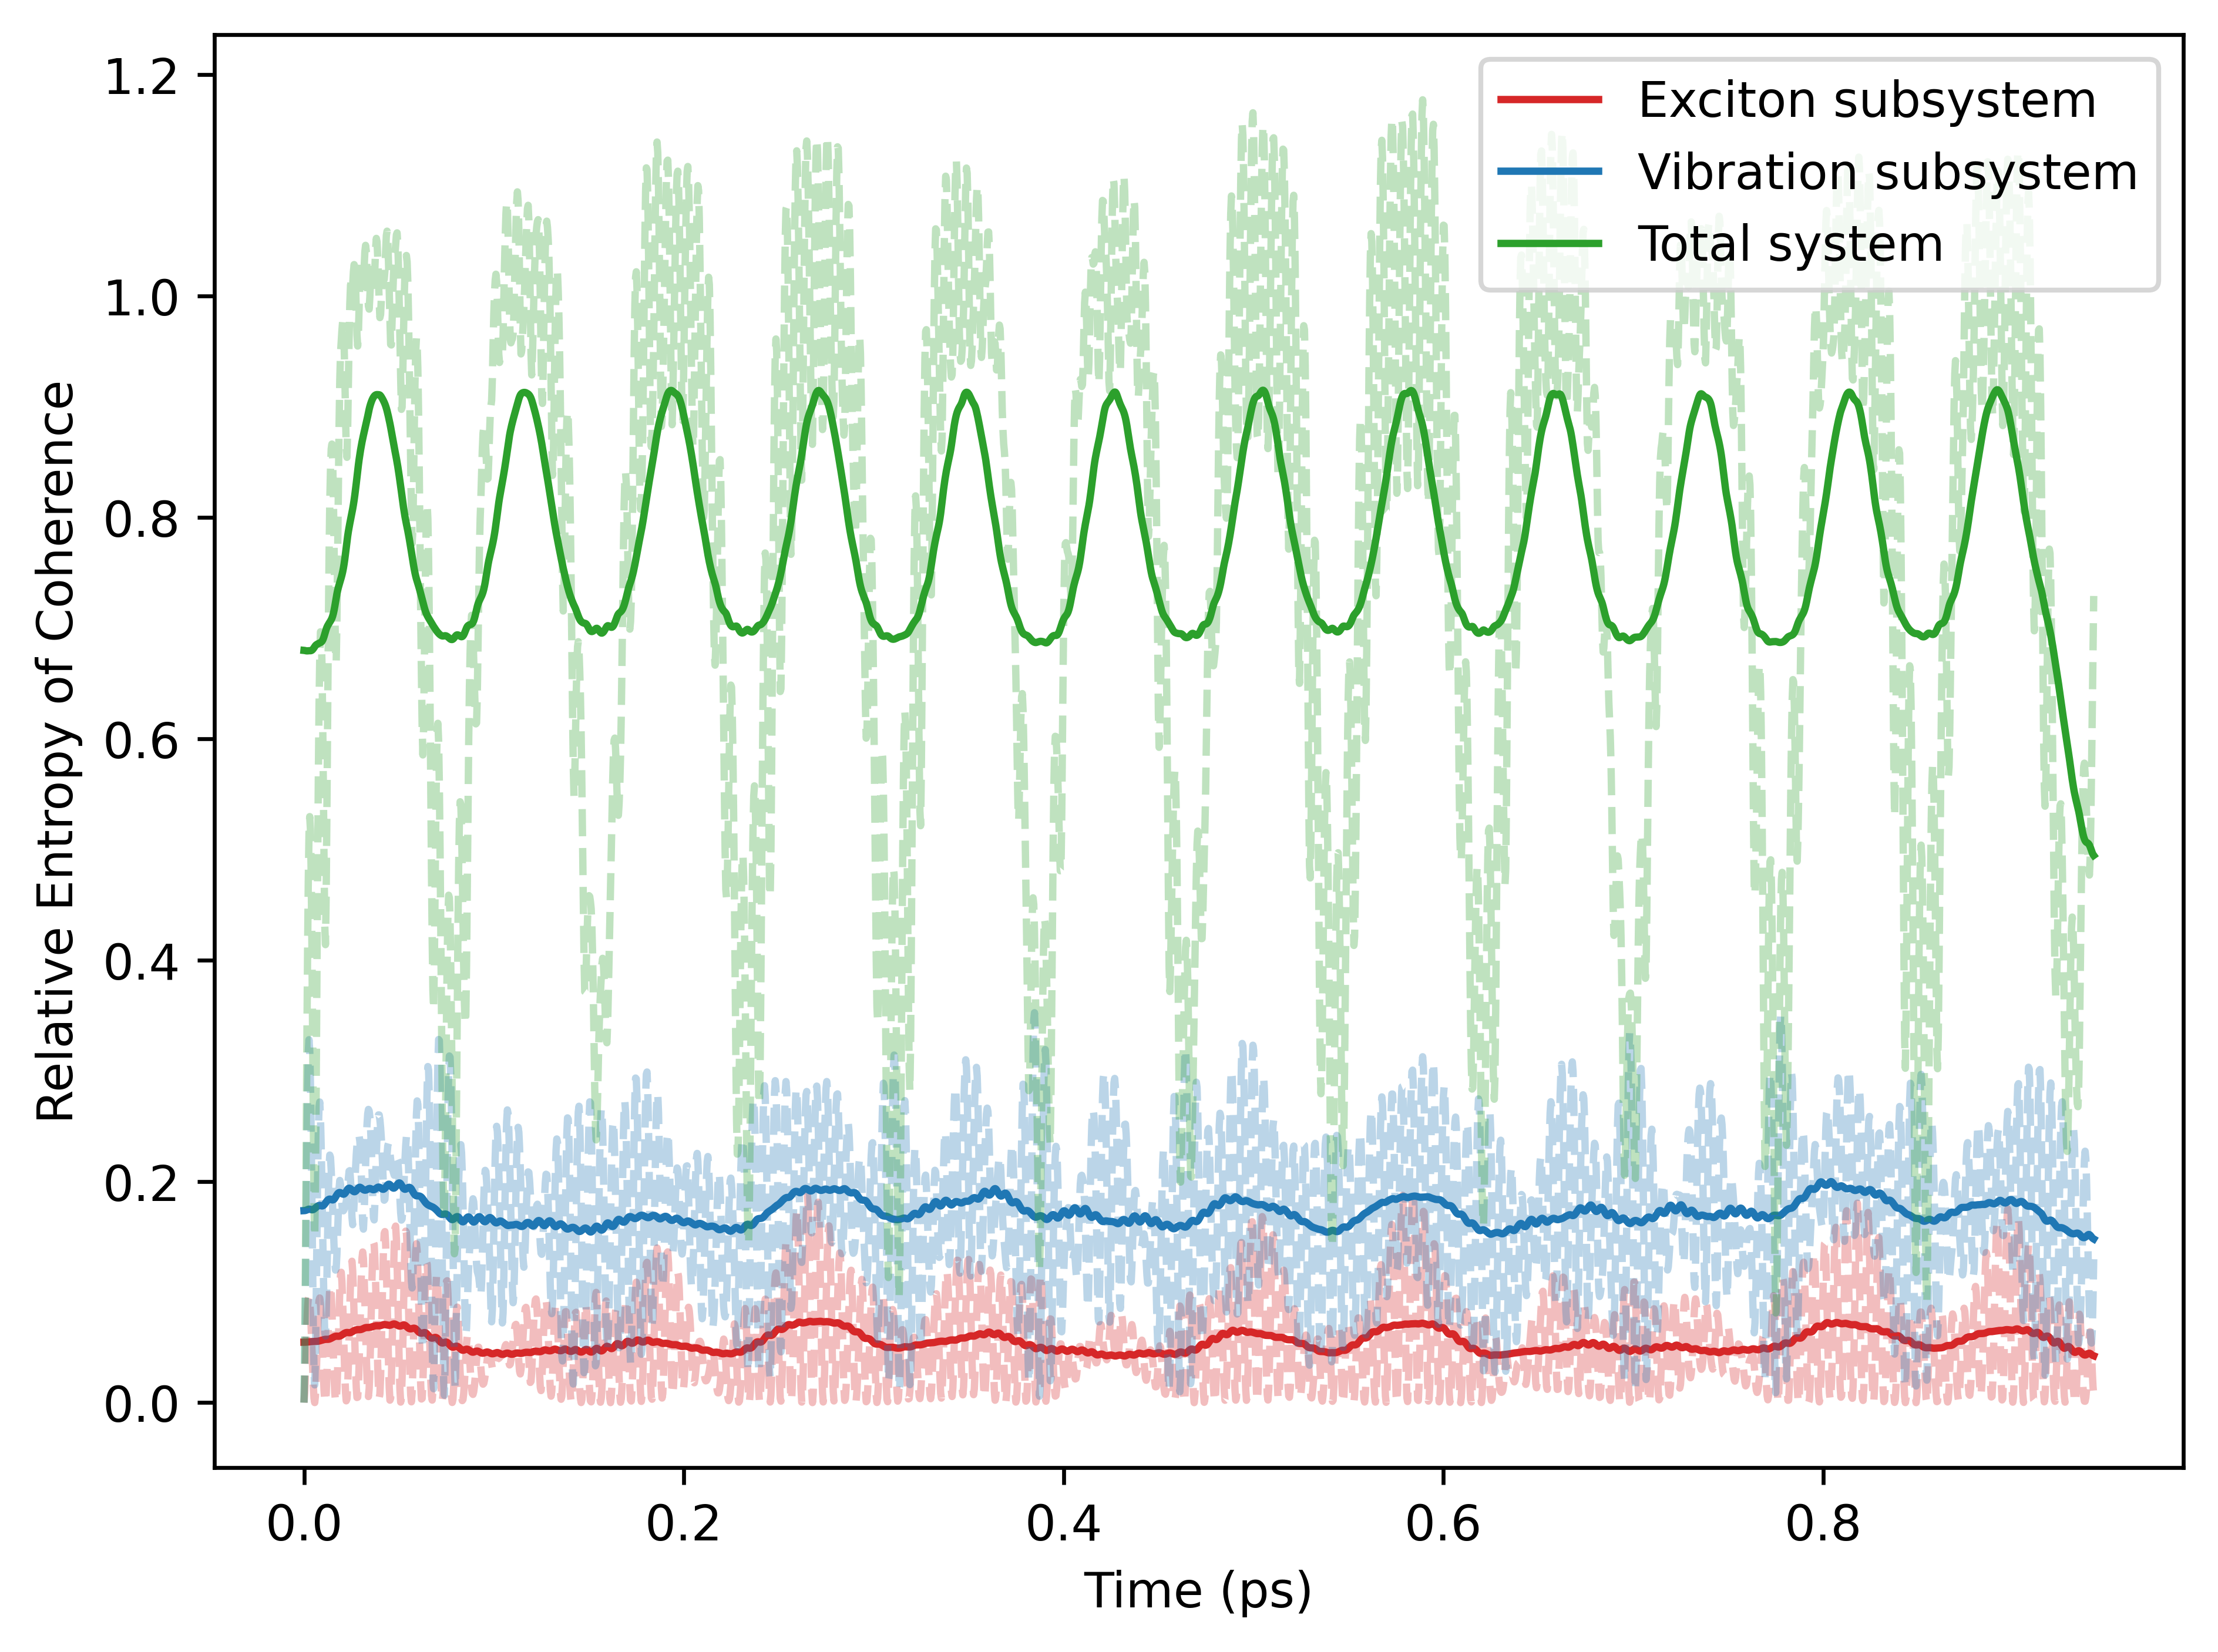
\includegraphics[width=\linewidth]{Research Project/Code/results/ExVib/Closed/Envelope/coh.png}
        \caption{}
        \label{fig:EVM_CQS_Coh_env}
    \end{subfigure}
    \hfill
    \begin{subfigure}{0.49\textwidth}
        \centering
        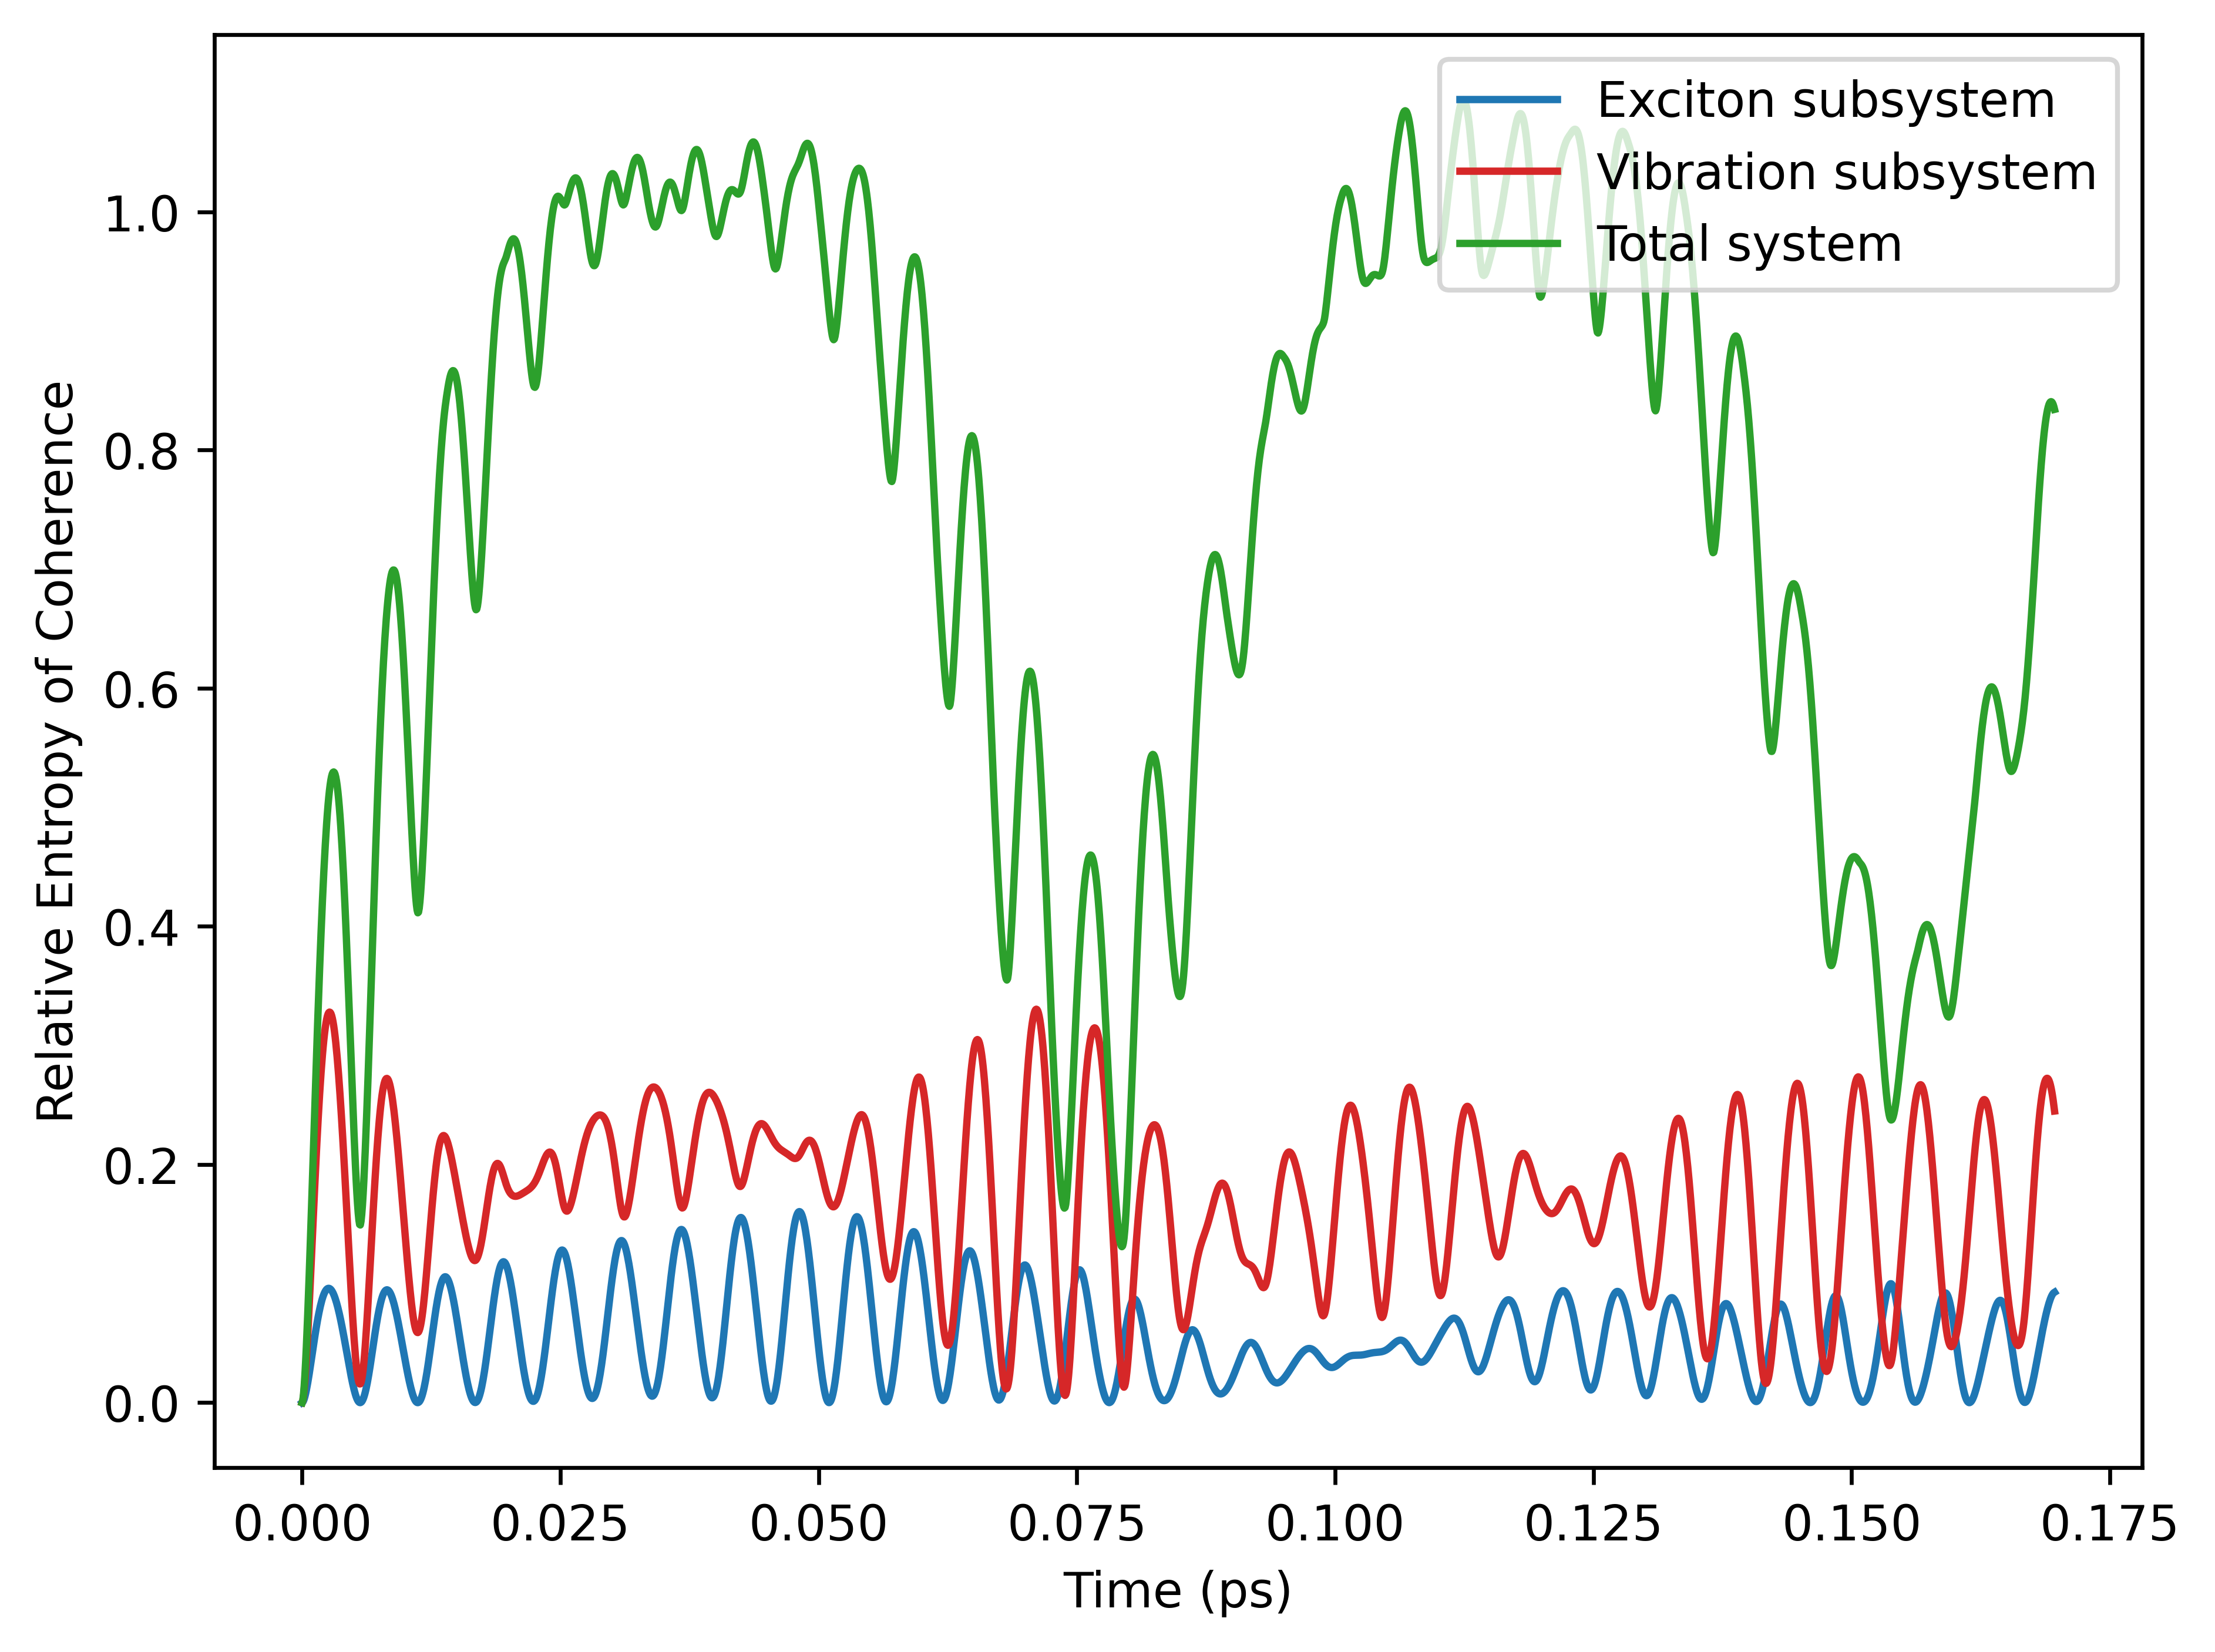
\includegraphics[width=\linewidth]{Research Project/Code/results/ExVib/Closed/Fast/coh.png}
        \caption{}
        \label{fig:EVM_CQS_Coh_fast}
    \end{subfigure}
    
    \caption{}
    \label{fig:EVM_CQS_Coh}
\end{figure}

%%%%%%%%%%%%%%%%%%%%%%%%
\begin{figure}[H]
    \centering
    \begin{subfigure}{0.49\textwidth}
        \centering
        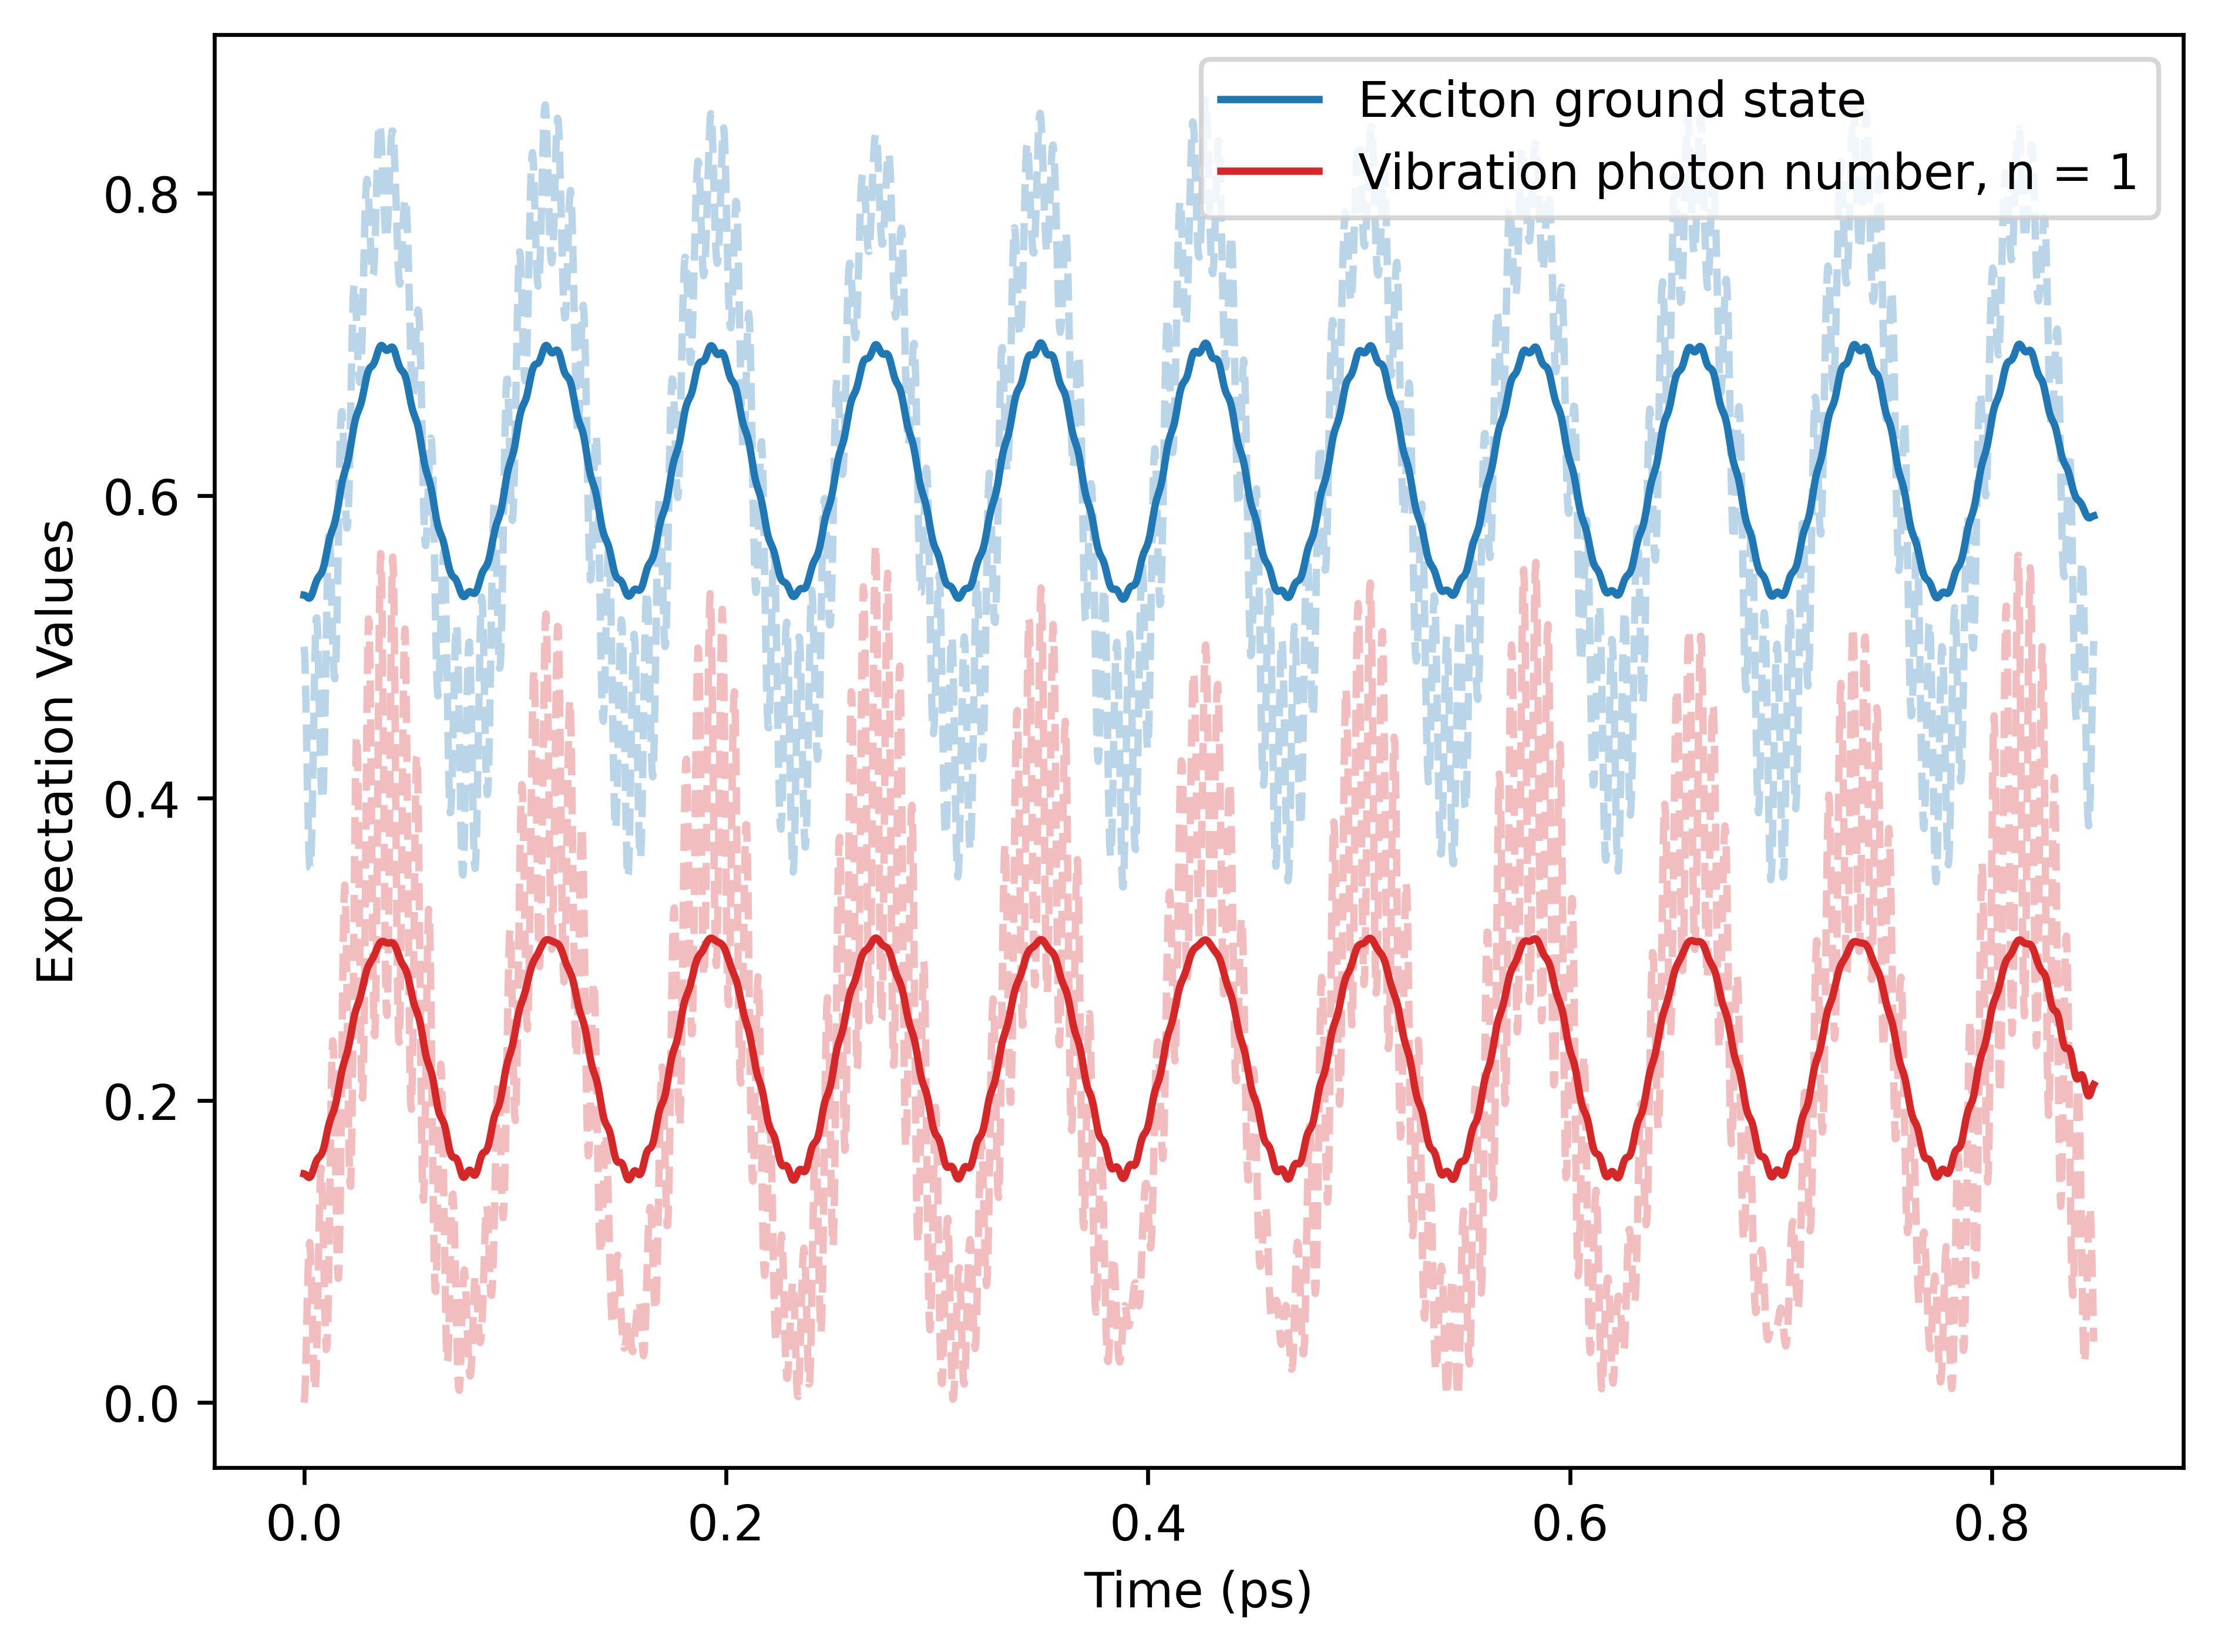
\includegraphics[width=\linewidth]{Research Project/Code/results/ExVib/Closed/Envelope/pops_ground_eg.png}
        \caption{}
        \label{fig:EVM_CQS_Pop_env_eg}
    \end{subfigure}
    \hfill
    \begin{subfigure}{0.49\textwidth}
        \centering
        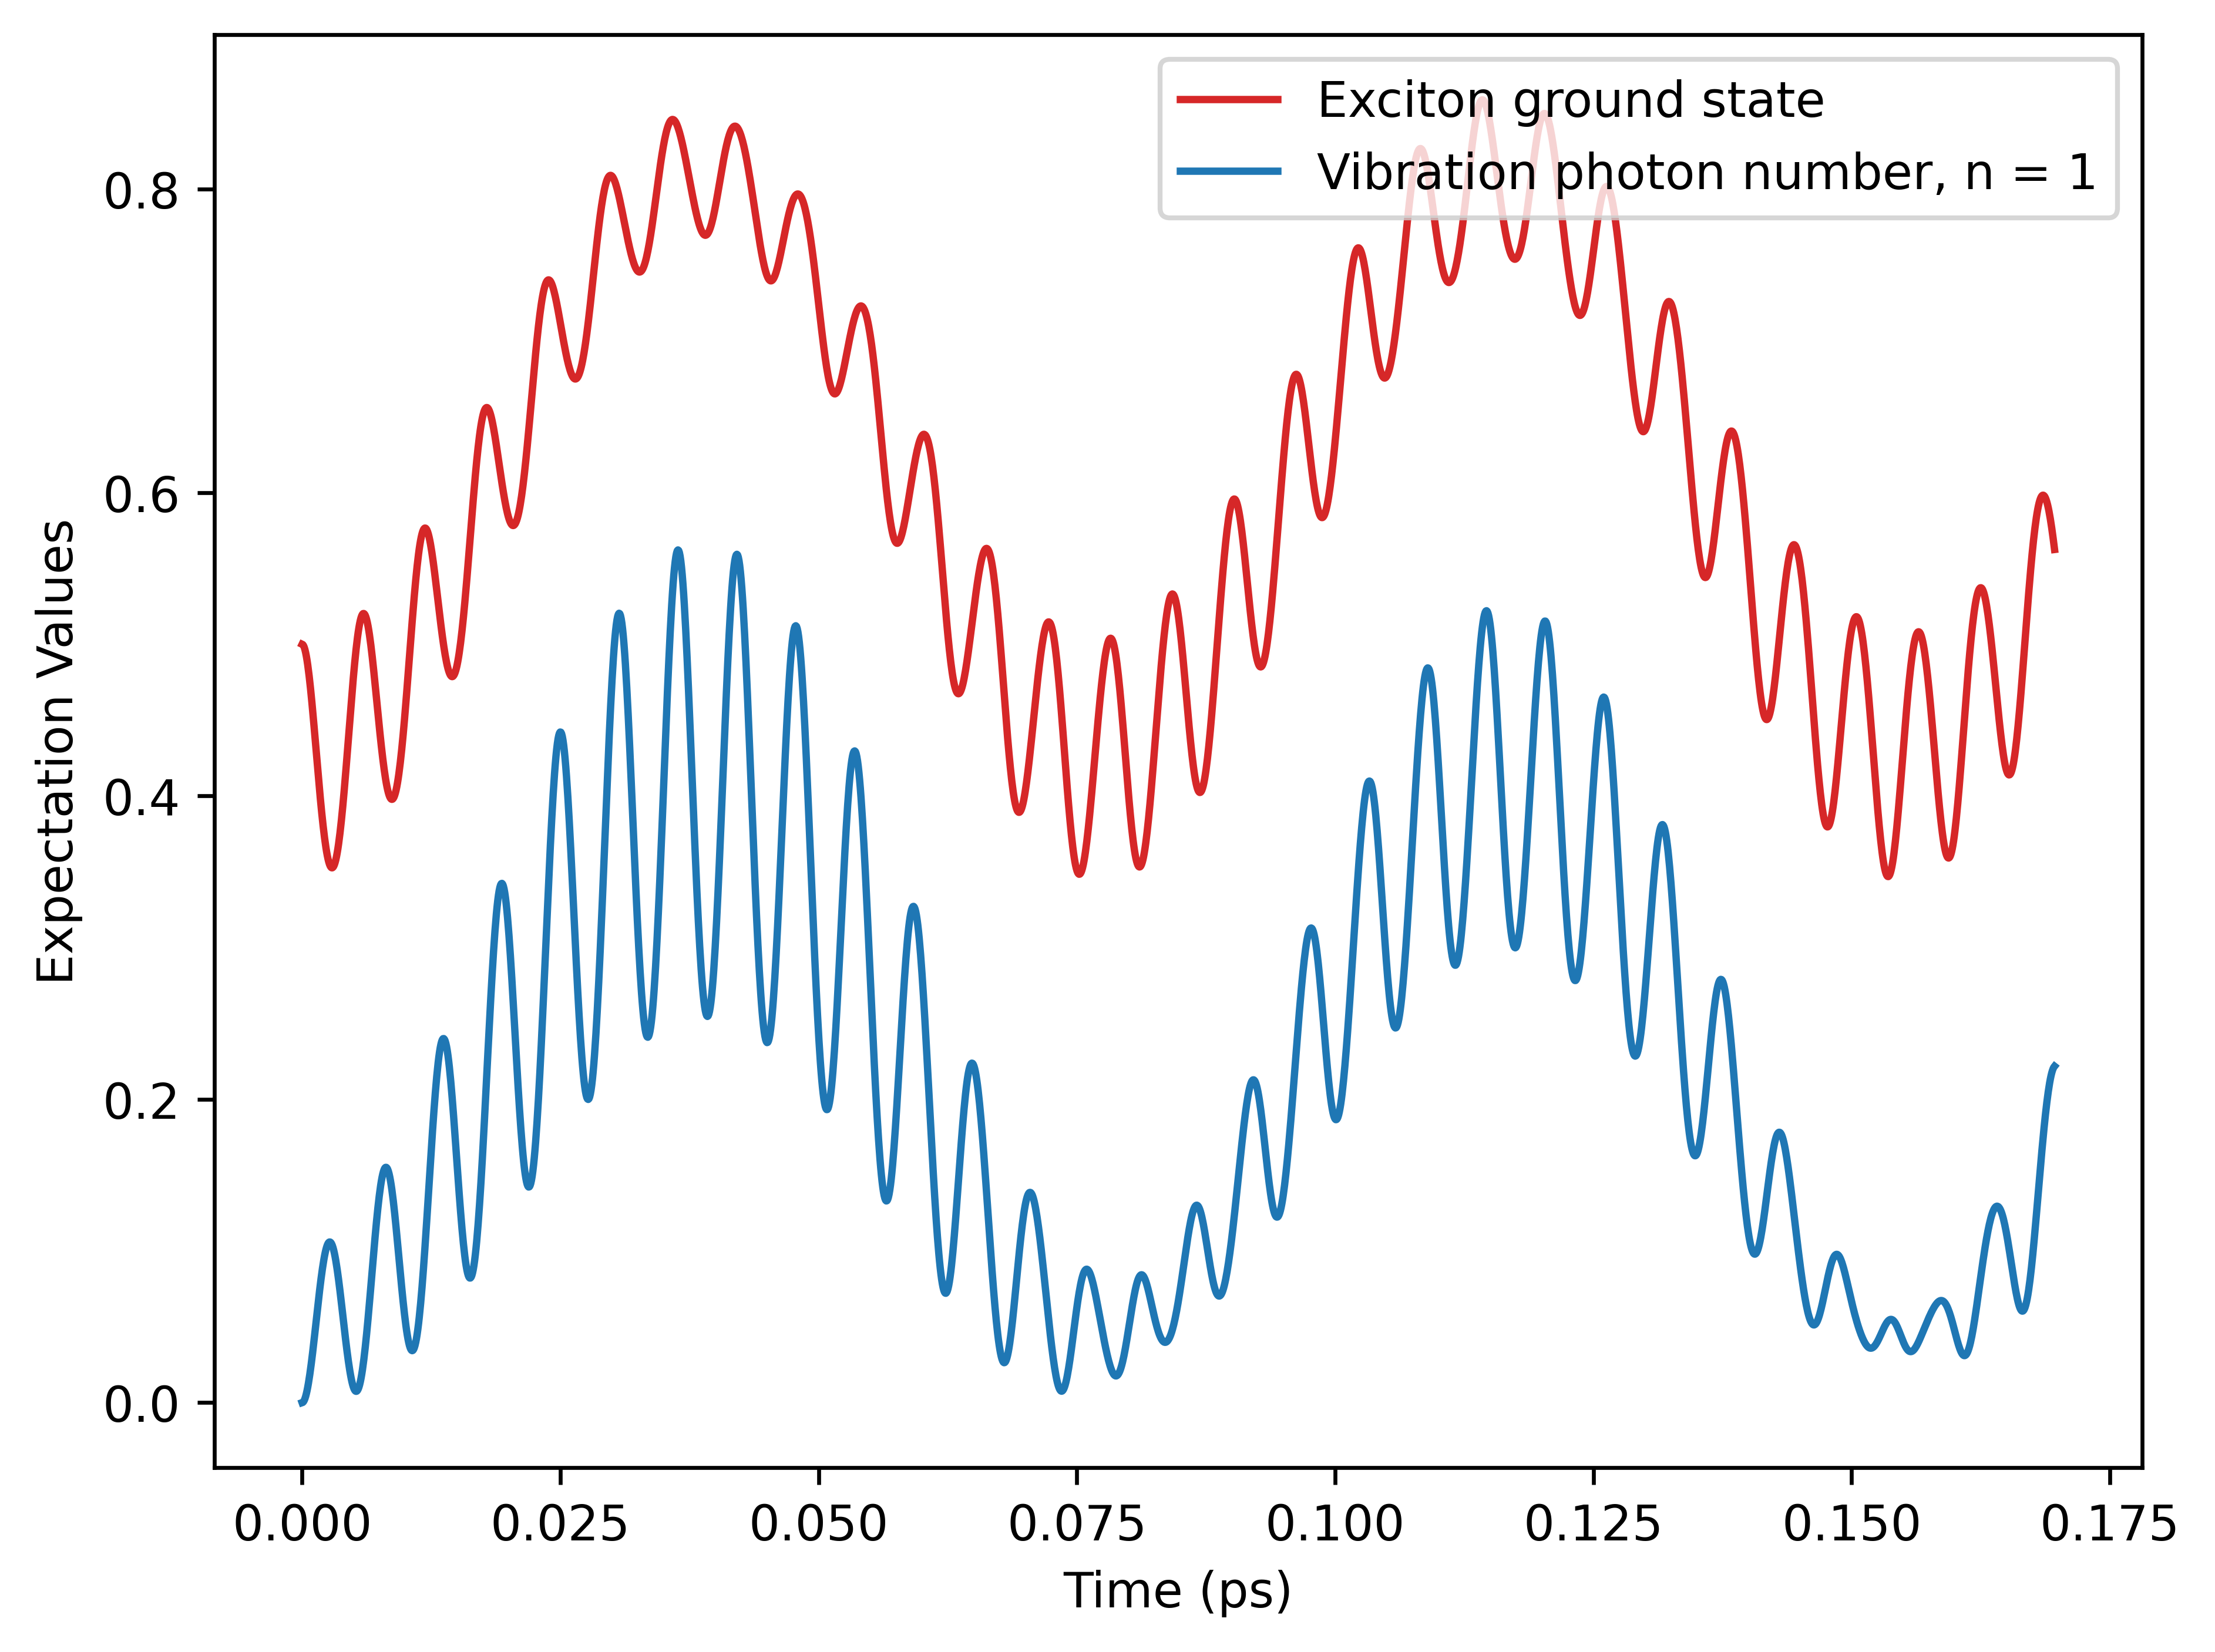
\includegraphics[width=\linewidth]{Research Project/Code/results/ExVib/Closed/Fast/pops_ground_eg.png}
        \caption{}
        \label{fig:EVM_CQS_Pop_fast_eg}
    \end{subfigure}
    
    \caption{}
    \label{fig:EVM_CQS_Pops_eg}
\end{figure}

\begin{figure}[H]
    \centering
    \begin{subfigure}{0.49\textwidth}
        \centering
        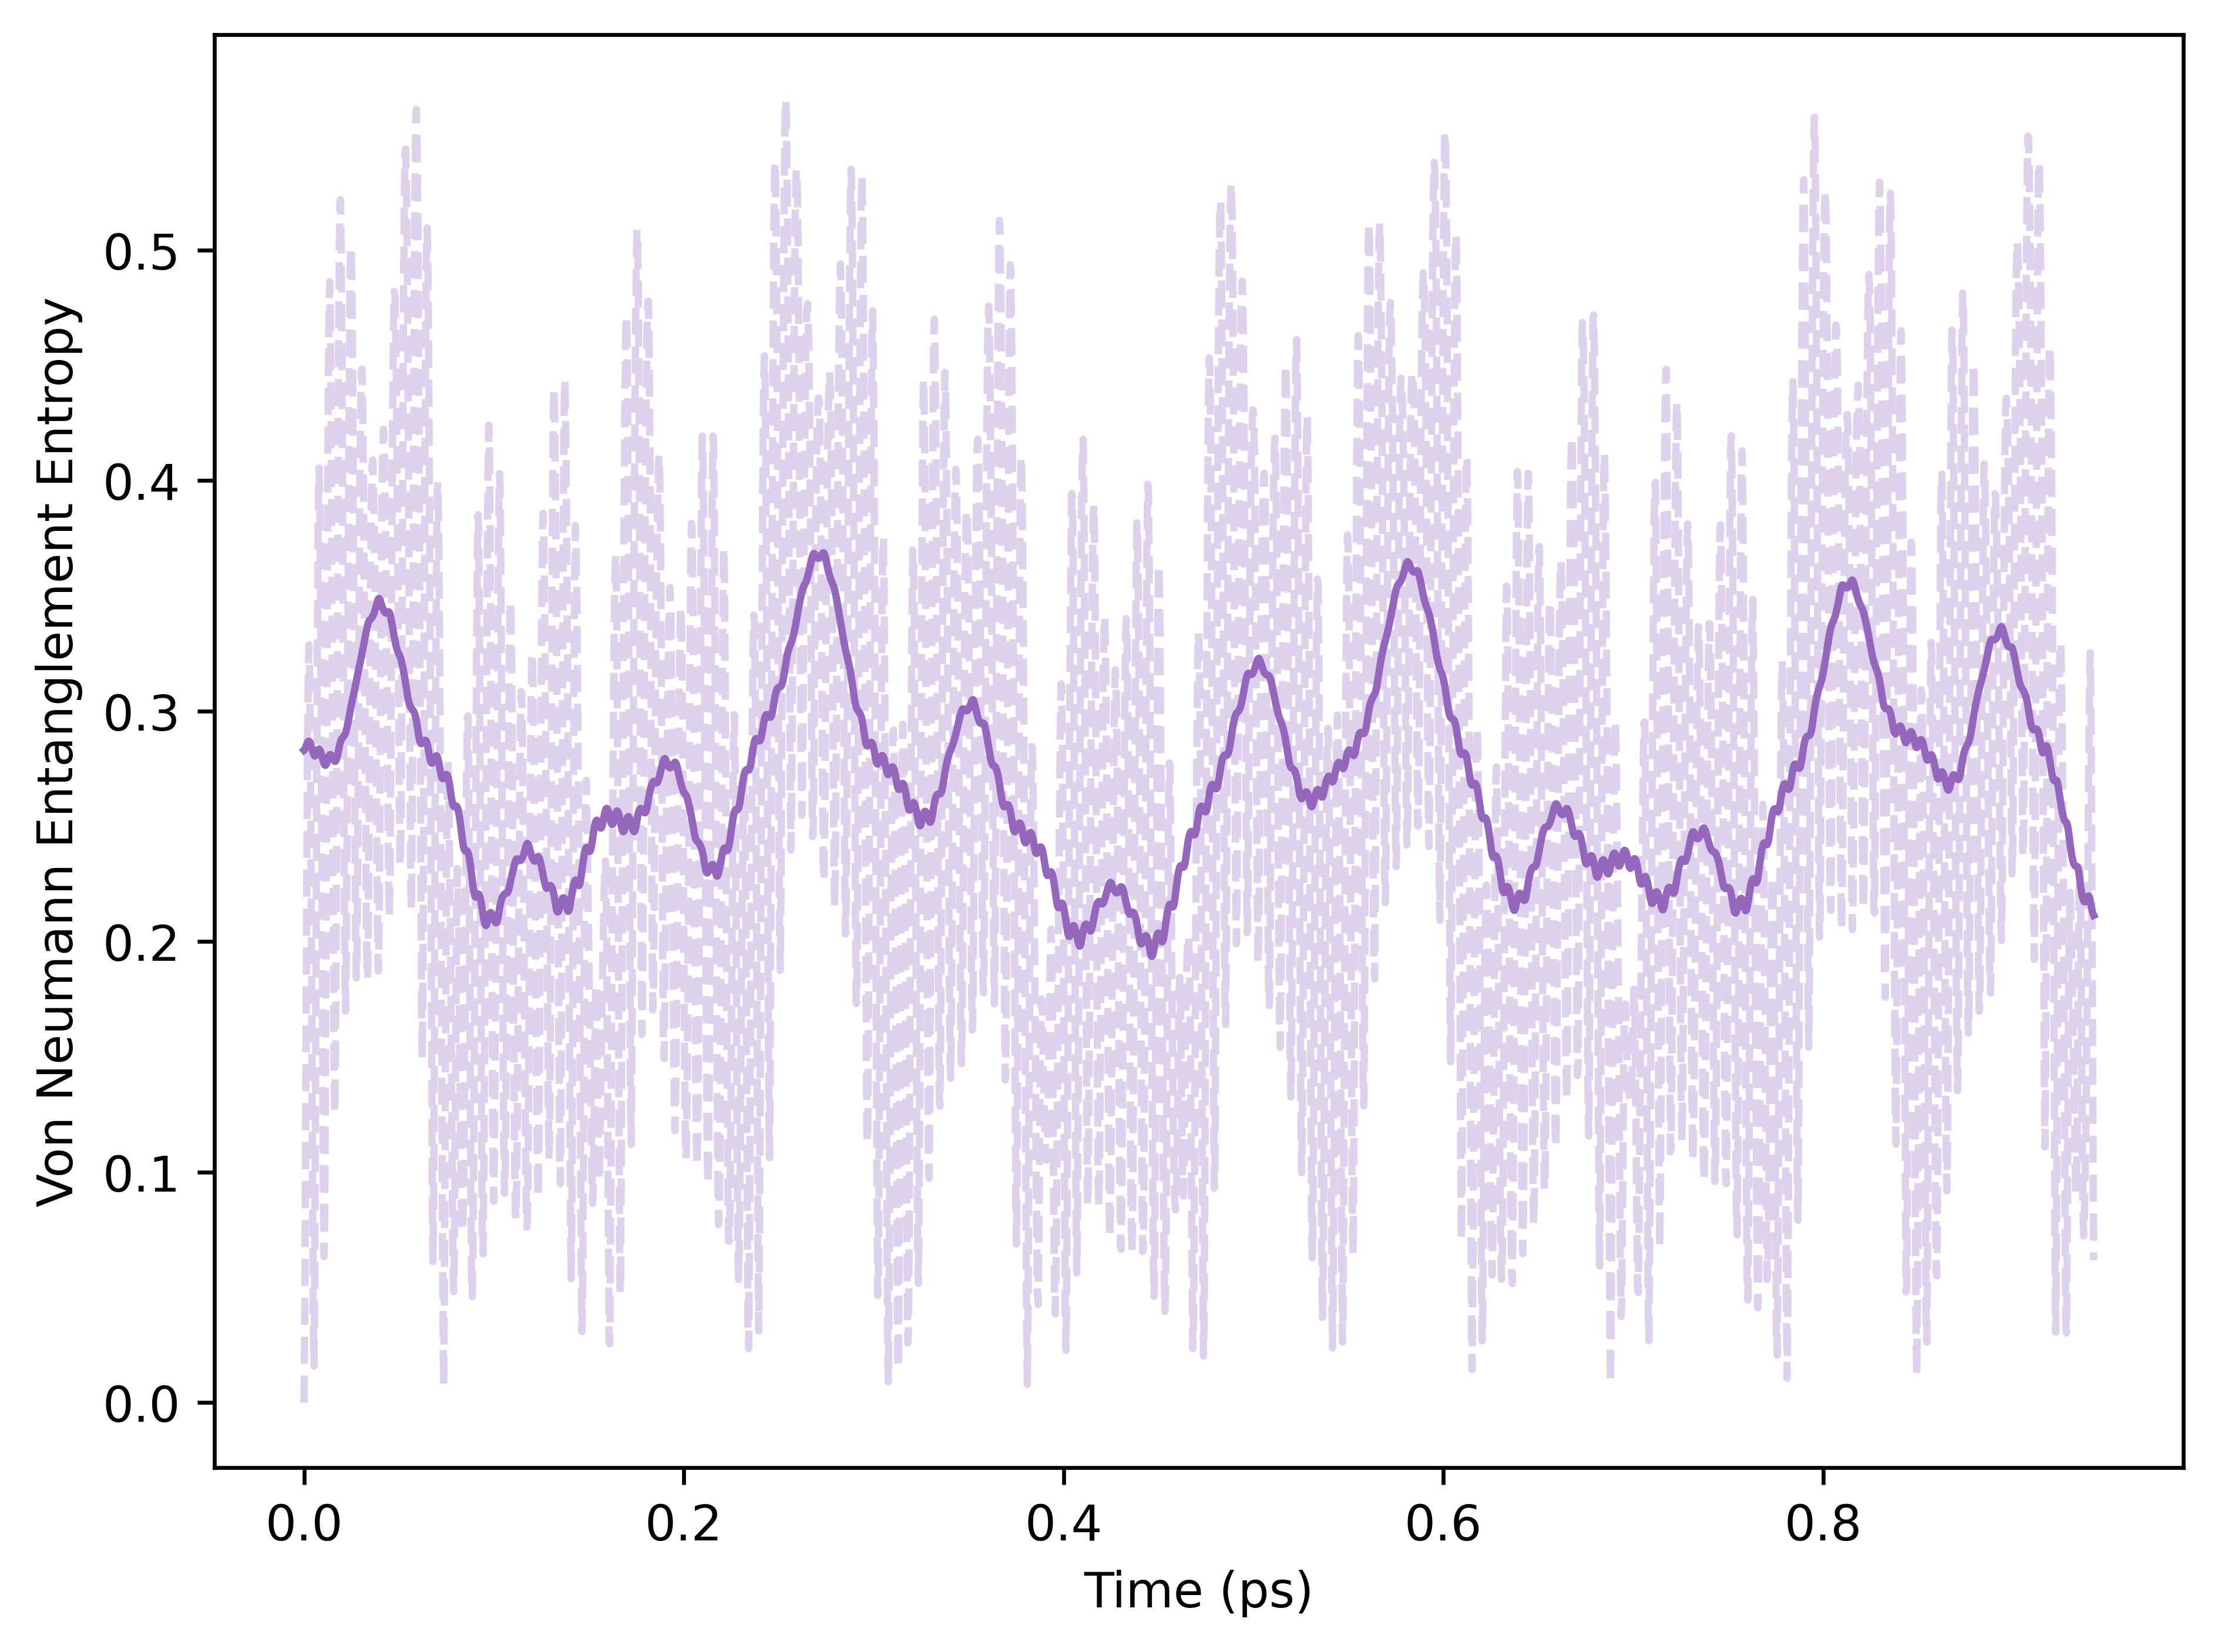
\includegraphics[width=\linewidth]{Research Project/Code/results/ExVib/Closed/Envelope/vne_eg.png}
        \caption{}
        \label{fig:EVM_CQS_Ent_env_eg}
    \end{subfigure}
    \hfill
    \begin{subfigure}{0.49\textwidth}
        \centering
        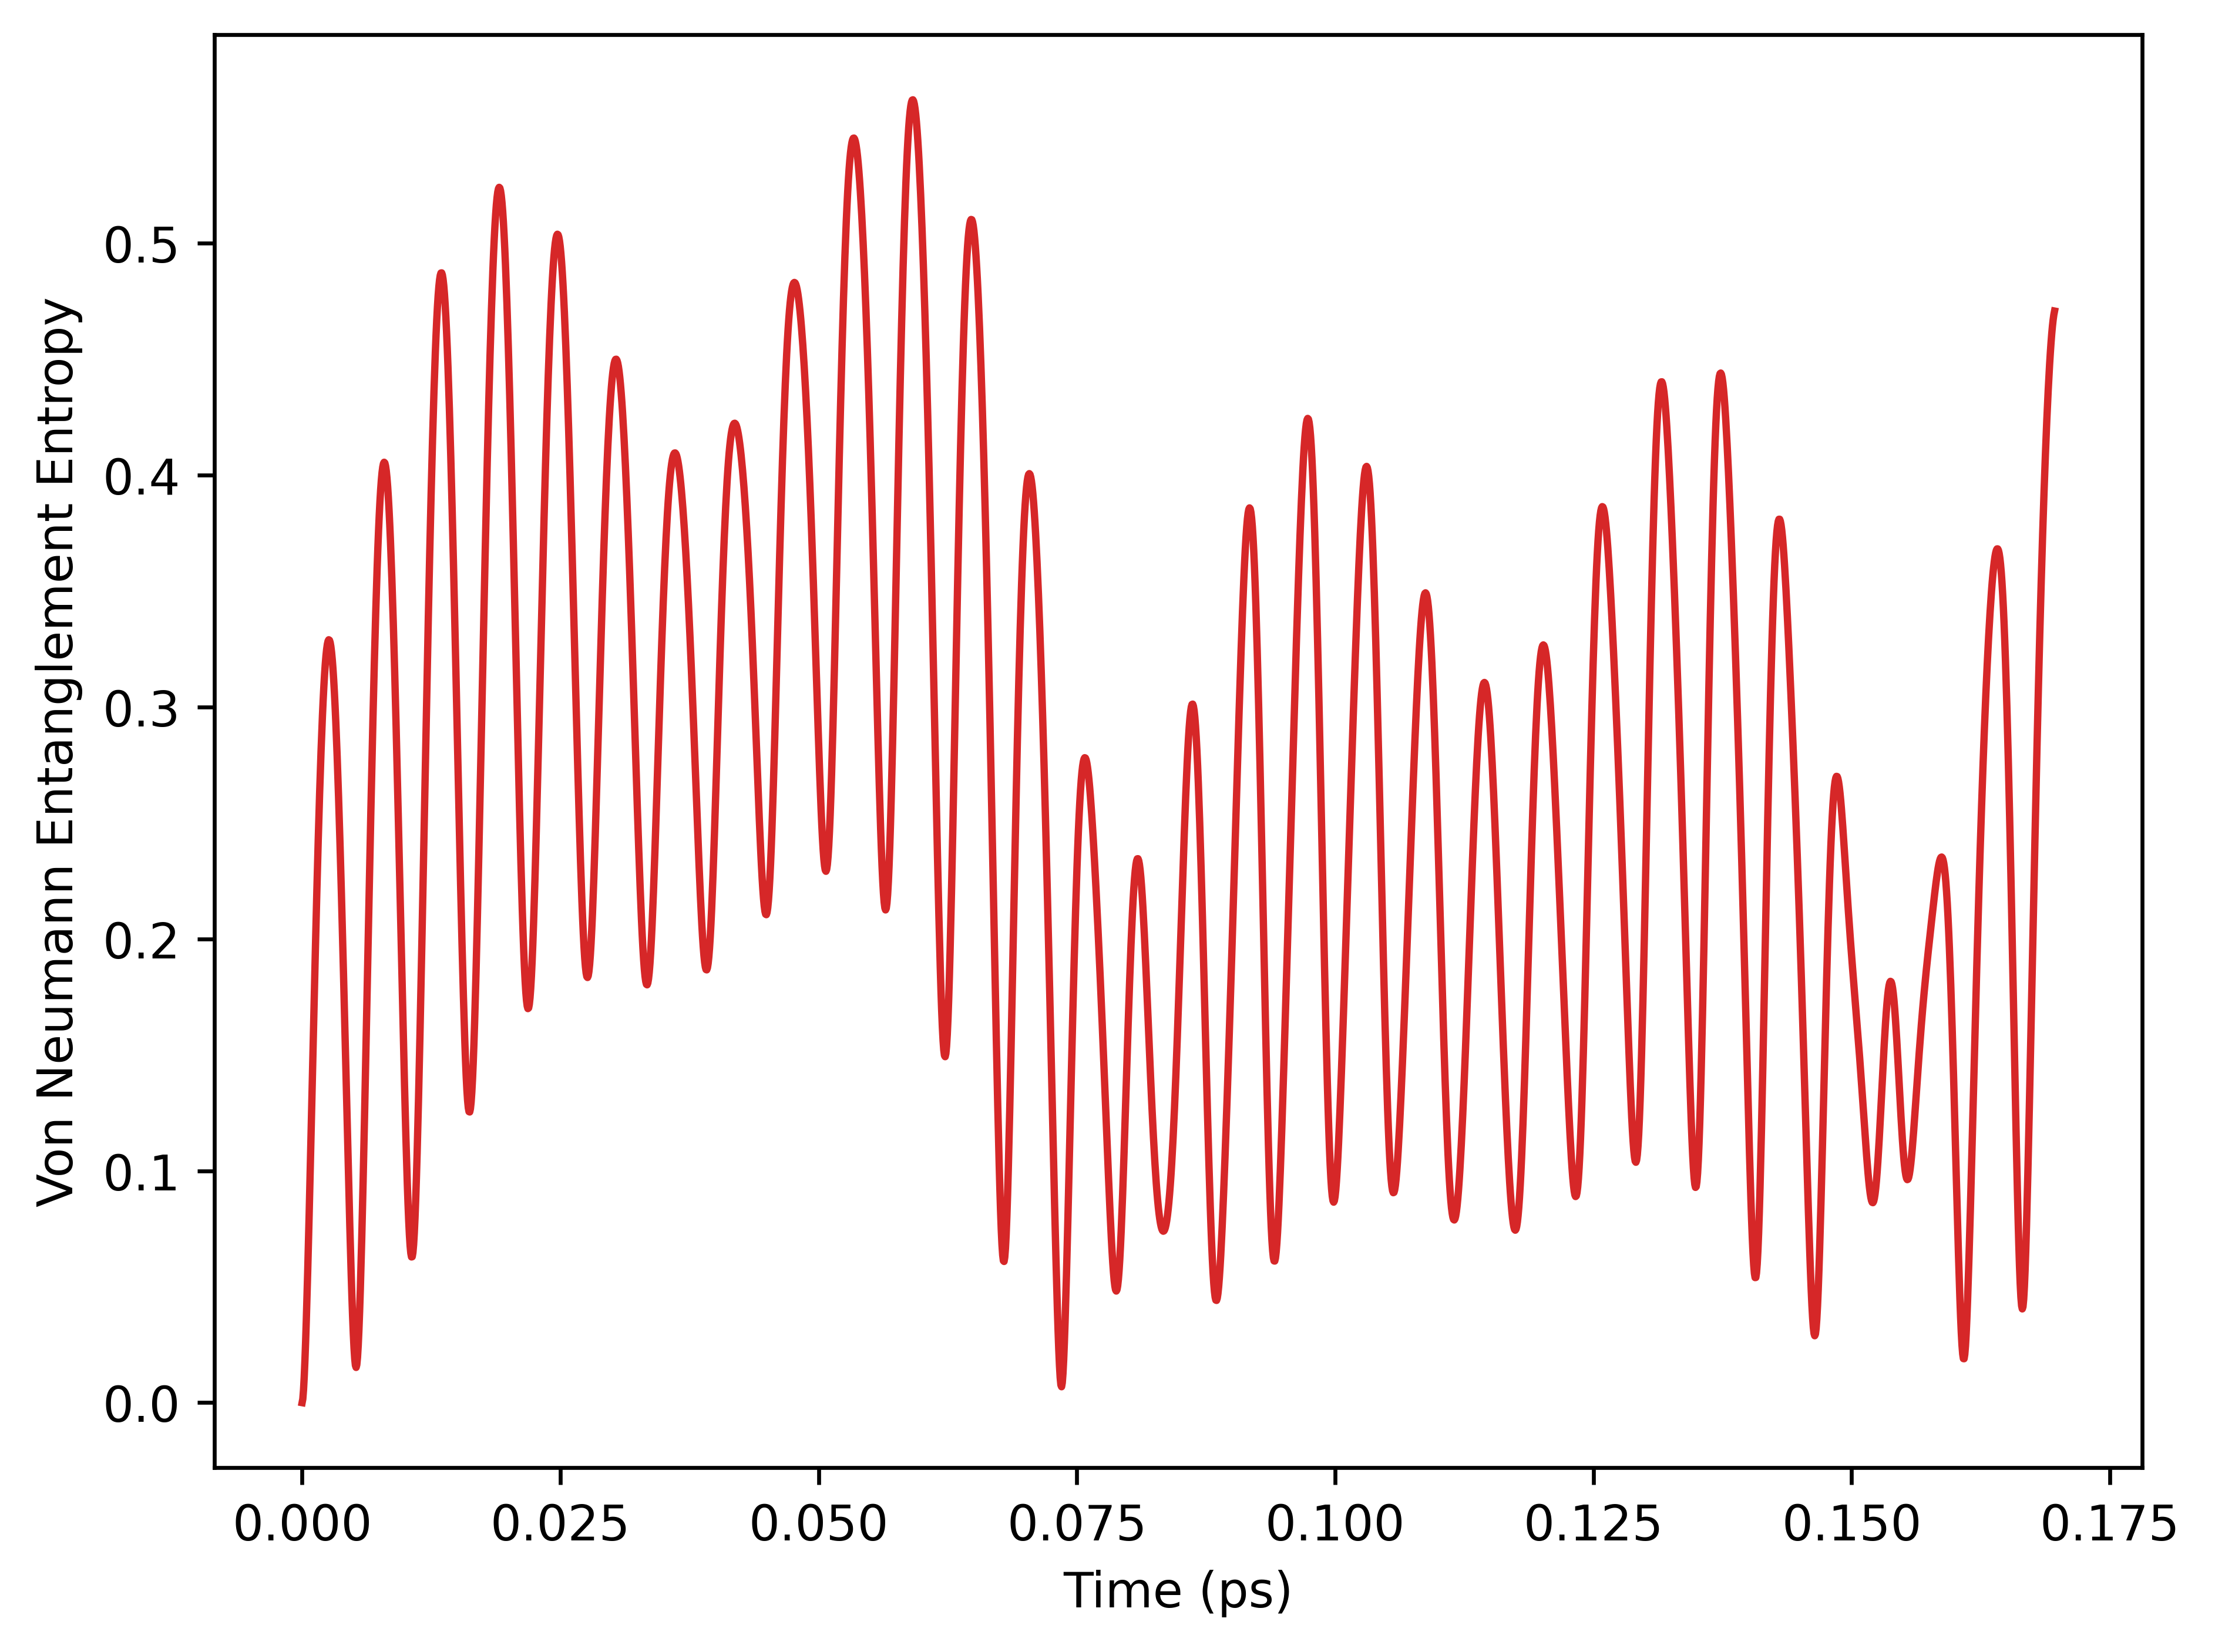
\includegraphics[width=\linewidth]{Research Project/Code/results/ExVib/Closed/Fast/vne_eg.png}
        \caption{}
        \label{fig:EVM_CQS_Ent_fast_eg}
    \end{subfigure}
    
    \caption{}
    \label{fig:EVM_CQS_Ent_eg}
\end{figure}

\begin{figure}[H]
    \centering
    \begin{subfigure}{0.49\textwidth}
        \centering
        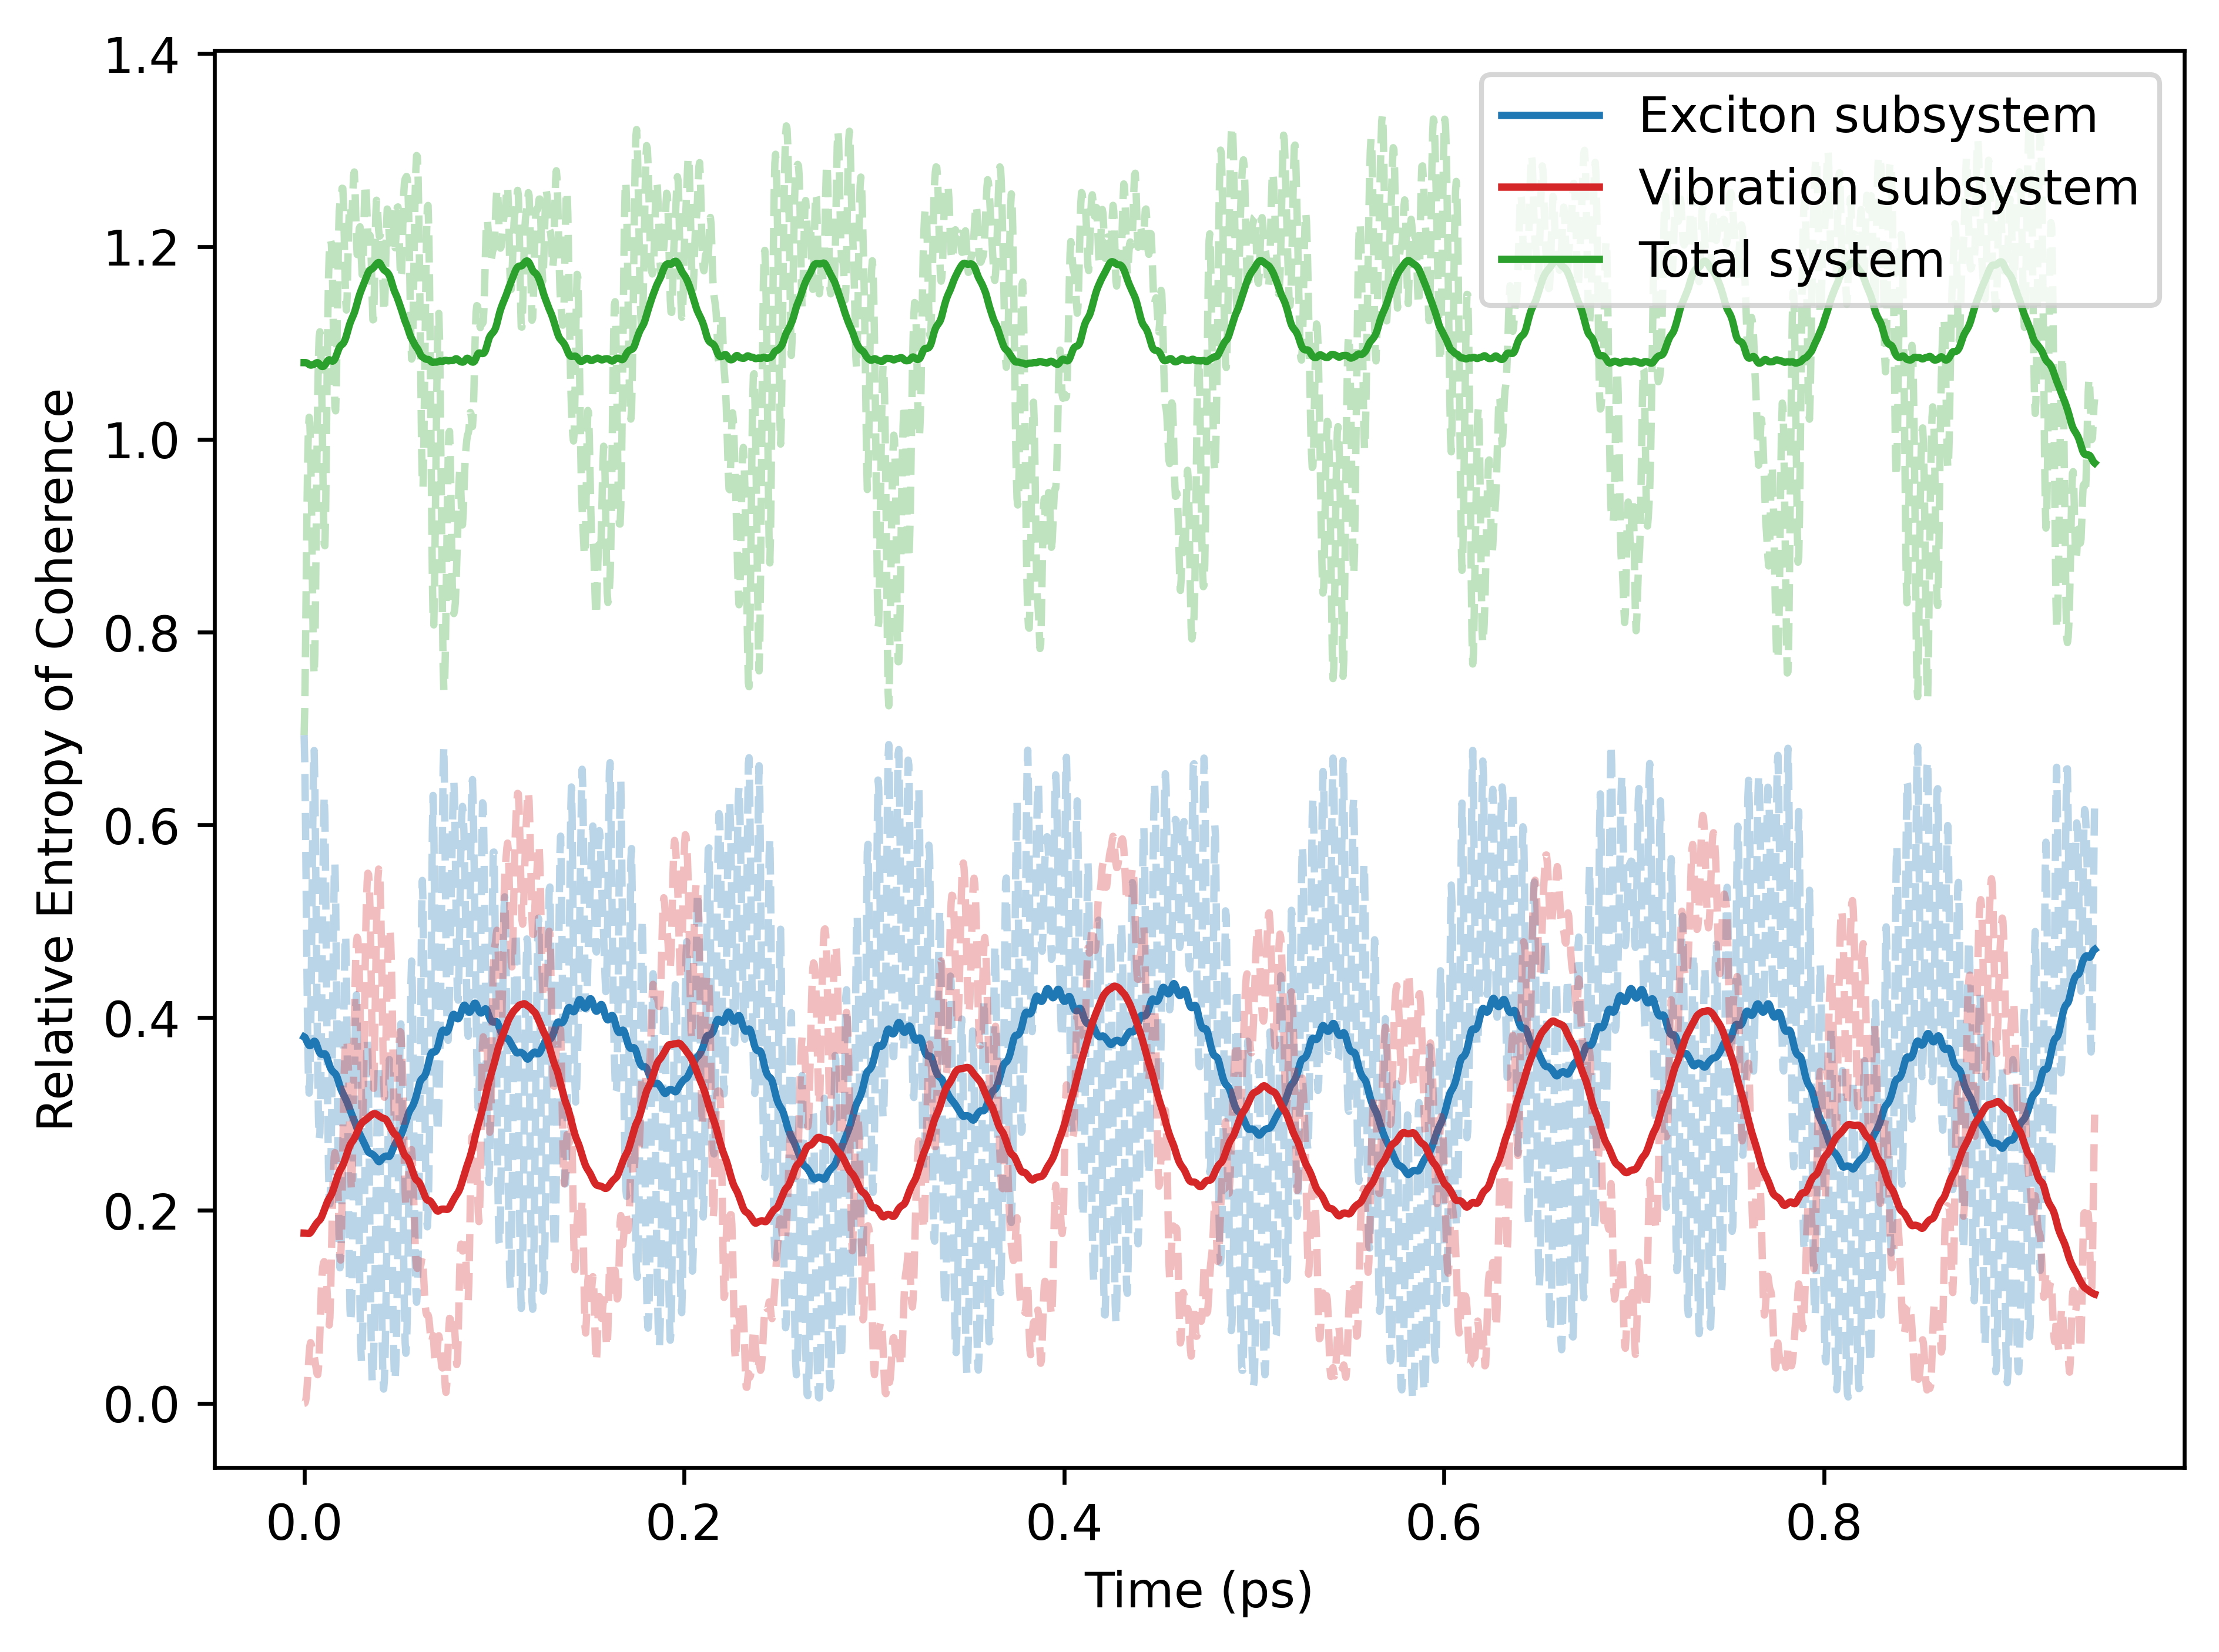
\includegraphics[width=\linewidth]{Research Project/Code/results/ExVib/Closed/Envelope/coh_eg.png}
        \caption{}
        \label{fig:EVM_CQS_Coh_env_eg}
    \end{subfigure}
    \hfill
    \begin{subfigure}{0.49\textwidth}
        \centering
        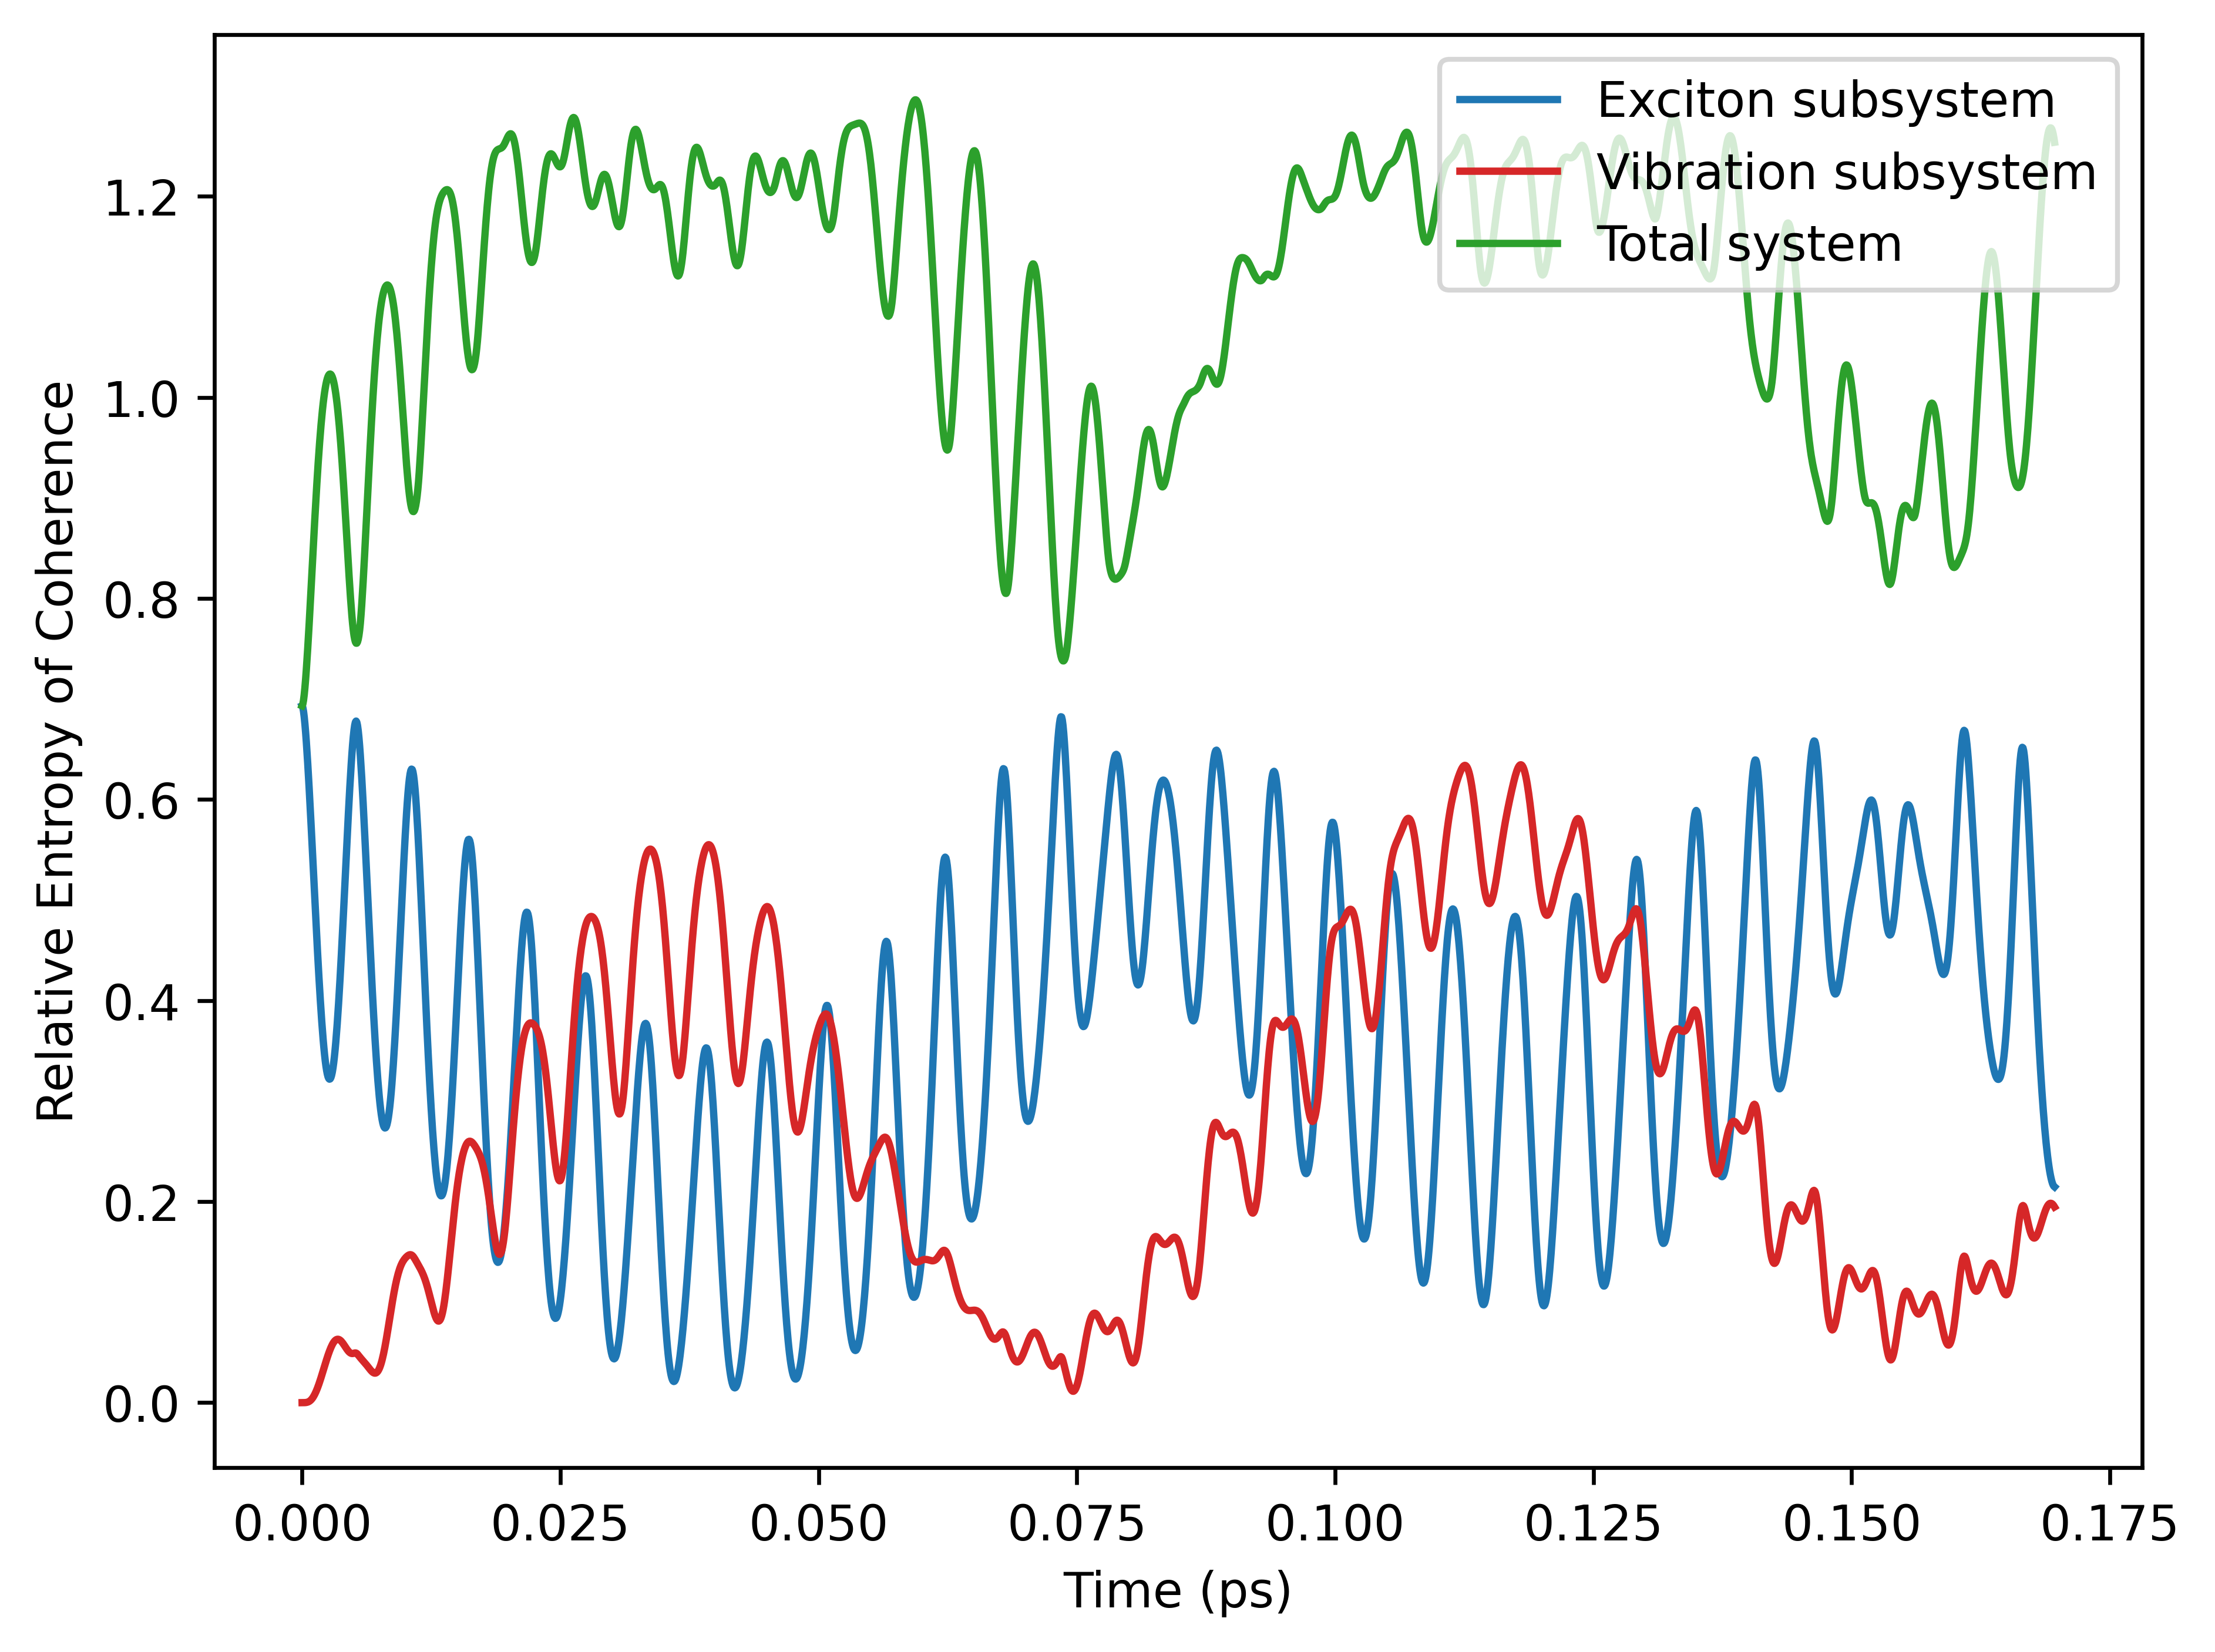
\includegraphics[width=\linewidth]{Research Project/Code/results/ExVib/Closed/Fast/coh_eg.png}
        \caption{}
        \label{fig:EVM_CQS_Coh_fast_eg}
    \end{subfigure}
    
    \caption{}
    \label{fig:EVM_CQS_Coh_eg}
\end{figure}

\subsubsection{Closed Evolution}
\subsubsection{Open Evolution}
\subsection{Discussion}




































%%%%%%%%%%%%%%%%%%%%%%%%%%%%%%%%%%%%%%%%%%%%% CONCLUSION %%%%%%%%%%%%%%%%%%%%%%%%%%%%%%%%%%%%%%%%%%%%%%%%%%%%%%
\newpage
\section{Conclusion and Outlook} \label{sec:conc}











































%%%%%%%%%%%%%%%%%%%%%%%%%%%%%%%%%%%%%%%%%%%%% Appendices %%%%%%%%%%%%%%%%%%%%%%%%%%%%%%%%%%%%%%%%%%%%%%%%%%%%%%
\begin{appendices}
    \section{Code Stuff} \label{appendix_code}
\end{appendices}
\newpage

\bibliographystyle{unsrt} 
\bibliography{References/references.bib} 

\end{document}